\documentclass[a4paper,14pt]{article}
\usepackage{extsizes} % для размера 14
\usepackage[english, russian]{babel} % переносы
\usepackage{graphicx} % для вставки картинок
\usepackage{fontspec} % шрифт Times
\setmainfont{Times New Roman}
\usepackage{indentfirst} % отступ первого абзаца
\setlength{\parindent}{1.25cm} % отступ первой строки
%\usepackage[onehalfspacing]{setspace}% полуторный интервал
%\renewcommand{\baselinestretch}{1.5}
\def\onehalflinespread{1.41}
\linespread{\onehalflinespread}
\frenchspacing % пробел после двоеточия
\usepackage{geometry} % поля
\usepackage{float} % перенос текста после рисунков
\floatplacement{figure}{H}
\geometry{left=3cm}
\geometry{right=1.5cm}
\geometry{top=2cm}
\geometry{bottom=2cm}
\sloppy % увеличение отступов между словами в строке при невозможности переноса
\usepackage[defaultlines=2,all]{nowidow} % абзац с новой страницы при нехватке места на заданное количество строк
\renewcommand{\labelitemi}{-} % тире в ненумерованных списках

\graphicspath{{images/}} % путь к изображениям
\renewcommand{\thefigure}{\thesection.\arabic{figure}} % шаблон номера рисунков
\renewcommand{\thetable}{\thesection.\arabic{table}} % шаблон номера таблиц
\newcommand{\newsection}{\clearpage\setcounter{figure}{0}\setcounter{table}{0}} % начало нового раздела 
\newcommand{\continuecaption}[1]{\caption*{#1}\\ \hline }
\newcommand{\centertocsection}[1]{\phantomsection\section*{#1}\addcontentsline{toc}{section}{#1} }

%\usepackage{longtable}
\usepackage{xltabular}
\usepackage{makecell}
\usepackage{setspace}
\renewcommand\theadfont{}
\newcolumntype{T}{>{\centering\arraybackslash}X} % новый тип столбца T - автоматическая ширина столбца с выравниванием по центру
\newcolumntype{R}{>{\raggedleft\arraybackslash}X} % новый тип столбца R - автоматическая ширина столбца с выравниванием по правому краю
\newcolumntype{C}[1]{>{\centering\let\newline\\\arraybackslash\hspace{0pt}}m{#1}} % новый тип столбца C - фиксированная ширина столбца с выравниванием по центру
\newcolumntype{r}[1]{>{\raggedleft\arraybackslash}p{#1}} % новый тип столбца r - фиксированная ширина столбца с выравниванием по правому краю
\newcommand{\centrow}{\centering\arraybackslash} % командой \centrow можно центрировать одну ячейку (заголовок) в столбце типа X или p, оставив в оcтальных ячейках другой тип выравнивания
\newcommand{\finishhead}{\endhead\hline\endlastfoot}
\usepackage{etoolbox}
\usepackage{totcount}
\newtotcounter{tablecnt}
\newtotcounter{figurecnt}

\def\toppad{4mm}
\def\tablepreskip{17.5pt}
\def\tablebelowskip{8.5pt}
\def\figurepreskip{21.5pt}
\def\figureaboveskip{10pt}
\def\figurebelowskip{8.5pt}

\setlength{\LTpre}{\tablepreskip}
\setlength{\LTpost}{\tablebelowskip}

\AtBeginEnvironment{xltabular}{\stepcounter{tablecnt}\renewcommand{\arraystretch}{\onehalflinespread}\linespread{1.0}\selectfont}

\AtBeginEnvironment{longtable}{\stepcounter{tablecnt}\vspace{5pt}}
\AfterEndEnvironment{longtable}{\vspace{7pt}}

\usepackage[tableposition=top]{caption} % подпись таблицы вверху
\captionsetup{strut=off}
\setlength{\intextsep}{0pt} % Vertical space above & below [h] floats
\setlength{\textfloatsep}{0pt} % Vertical space below (above) [t] ([b]) floats
\DeclareCaptionLabelFormat{gostfigure}{Рисунок #2} %подпись рисунка
\DeclareCaptionLabelFormat{gosttable}{Таблица #2} %подпись таблицы
\DeclareCaptionLabelSeparator{gost}{~--~} %разделитель в рисунках и таблицах
\captionsetup{labelsep=gost}
\captionsetup[figure]{aboveskip=\figureaboveskip,belowskip=\figurebelowskip,justification=centering,labelformat=gostfigure}
\captionsetup[table]{font={stretch=\onehalflinespread},skip=0pt,belowskip=0pt,aboveskip=8.5pt,singlelinecheck=off,labelformat=gosttable}

\usepackage{titlesec}

\titleformat{name=\section,numberless}[block]
{\normalsize\filcenter}
{}
{0pt}{}  %настройка ненумерованного раздела (Введение, содержание)

\titleformat{\section}[block] %настройка заголовка раздела
{\normalsize\bfseries}
{\hspace{1.25cm}\thesection}
{1em}{}

\titleformat{\subsection}[block]  %настройка заголовка подраздела
{\normalsize\bfseries}
{\hspace{1.25cm}\thesubsection}
{1em}{}
\setlength\leftmarginii  {0pt}

\titleformat{\subsubsection}[block]
{\normalsize\bfseries}
{\hspace{1.25cm}\thesubsubsection}
{1em}{}

\titleformat{\paragraph}[block]
{\normalsize\bfseries}
{\hspace{1.25cm}\theparagraph}
{1em}{}

\titlespacing*{name=\section,numberless}{0pt}{\toppad}{\toppad} % отступы разделов
\titlespacing*{\section}{0pt}{\toppad}{\toppad}
\titlespacing*{\subsection}{0pt}{\toppad}{\toppad}
\titlespacing*{\subsubsection}{0pt}{\toppad}{\toppad}
\titlespacing*{\paragraph}{0pt}{\toppad}{\toppad}
\usepackage{array} % новый вид колонки с выравниванием по центру

\usepackage{enumitem}
\setlist{nolistsep,wide=\parindent,itemindent=*} % отступы вокруг списков, выравнивание с учетом разделителя

\usepackage[]{tocloft}
\setlength{\cftbeforetoctitleskip}{-1em}
\addto\captionsrussian{
	\renewcommand\contentsname{}
}
\renewcommand{\cftdot}{} % убрать отточие
\renewcommand{\cftsecfont}{\normalsize} % не жирный шрифт раздела в оглавлении
\renewcommand{\cftsecpagefont}{\textmd} % не жирный номер страницы для раздела
\setcounter{tocdepth}{4} % число уровней оглавления
\setcounter{secnumdepth}{4} % число уровней подразделов

\def\secwidth{0pt}
\setlength{\cftsecnumwidth}{\secwidth}
\setlength{\cftsubsecnumwidth}{\secwidth}
\setlength{\cftsubsubsecnumwidth}{\secwidth}
\setlength{\cftparanumwidth}{\secwidth}
\setlength{\cftbeforesecskip}{0pt} % интервал между разделами содержания
\setlength{\cftsecindent}{0pt}% Remove indent for \section
\setlength{\cftsubsecindent}{0pt}% Remove indent for \subsection
\setlength{\cftsubsubsecindent}{0pt}% Remove indent for \subsubsection
\setlength{\cftparaindent}{0pt}% Remove indent for \paragraph

\def\secindent{3.8em}
\renewcommand{\cftsecaftersnumb}{\hspace{\secindent}}
\renewcommand{\cftsubsecaftersnumb}{\hspace{\secindent}}
\renewcommand{\cftsubsubsecaftersnumb}{\hspace{\secindent}}
\renewcommand{\cftparaaftersnumb}{\hspace{\secindent}}

\makeatletter
\renewcommand\@biblabel[1]{#1.} %оформление элемента списка литературы
\renewenvironment{thebibliography}[1]
{\list{\@biblabel{\@arabic\c@enumiv}}%
	{\settowidth\labelwidth{\@biblabel{#1}}%
		\leftmargin\labelwidth
		\setlength{\topsep}{0pt}                  
		\setlength{\partopsep}{0pt}
		\setlength{\itemsep}{0pt}
		\setlength{\parsep}{0pt}
		\setlength{\parskip}{0pt}
		\setlength{\itemindent}{1.75cm}
		\setlength{\leftmargin}{0pt}
		\@openbib@code
		\usecounter{enumiv}%
		\let\p@enumiv\@empty
		\renewcommand\theenumiv{\@arabic\c@enumiv}}%
	\sloppy
	\clubpenalty4000
	\interlinepenalty10000 %запрет переноса элемента на новую страницу
	\@clubpenalty \clubpenalty
	\widowpenalty4000%
	\sfcode`\.\@m}
{\def\@noitemerr
	{\@latex@warning{Empty `thebibliography' environment}}%
	\endlist}

\newsavebox\saved@arstrutbox 
\newcommand*{\setarstrut}[1]{% команда для уменьшения высоты строки в таблице
	\noalign{%
		\begingroup
		\global\setbox\saved@arstrutbox\copy\@arstrutbox
		#1%
		\global\setbox\@arstrutbox\hbox{%
			\vrule \@height\arraystretch\ht\strutbox
			\@depth\arraystretch \dp\strutbox
			\@width\z@
		}%
		\endgroup
	}%
}
\newcommand*{\restorearstrut}{% восстановление высоты строки
	\noalign{%
		\global\setbox\@arstrutbox\copy\saved@arstrutbox
	}%
}

\makeatother

% Раскомментировать блок при необходимости использования страниц с альбомной ориентацией. Предпочтительнее их не использовать, а осуществлять поворт рисунков на 90 градусов.
%
%Пример использования:
%
%%\begin{albumpage}
%%	\begin{figure}
%	%		\centering
%	%%		\vskip 1.0cm %способ добавить отступ, если необходимо
%	%		\includegraphics[height=0.95\textheight]{img/precedents_common}
%	%		\caption{Диаграмма прецедентов}
%	%		\label{fig:precedentscommon}
%	%	\end{figure}
%%\end{albumpage}
%
%\newbool{onalbumpage}
%\setbool{onalbumpage}{false}
%\BeforeBeginEnvironment{figure}{%
%	\ifbool{onalbumpage}{% true part:
%	}{
%		\stepcounter{figurecnt}\addvspace{\figurepreskip}
%	}
%}
%
%\usepackage{lscape}
%\usepackage{pdflscape}
%\usepackage{everypage}
%
%\newlength{\hfoot}
%\newlength{\vfoot}
%\AddEverypageHook{\ifdim\textwidth=\linewidth\relax
%	\else\setlength{\hfoot}{-\topmargin}%
%	\addtolength{\hfoot}{-\headheight}%
%	\addtolength{\hfoot}{-\headsep}%
%	\addtolength{\hfoot}{-.5\linewidth}%
%	\ifodd\value{page}\setlength{\vfoot}{\oddsidemargin}%
%	\else\setlength{\vfoot}{\evensidemargin}\fi%
%	\addtolength{\vfoot}{\textheight}%
%	\addtolength{\vfoot}{\footskip}%
%	\raisebox{\hfoot}[0pt][0pt]{\rlap{\hspace{.981\vfoot}\rotatebox[origin=cB]{90}{\thepage}}}\fi}
%
%\newenvironment{albumpage}{
%	\captionsetup[figure]{belowskip=0pt}
%	\setbool{onalbumpage}{true}
%%	\newgeometry{left=2cm,right=2cm,top=1.5cm,bottom=3cm}
%	\begin{landscape}
%		\pagestyle{empty}
%}{
%	\end{landscape}
%	\pagestyle{plain}
%%	\restoregeometry
%	\setbool{onalbumpage}{false}
%	\captionsetup[figure]{belowskip=\figurebelowskip}
%}
%
% Закомментировать строку ниже
%
\BeforeBeginEnvironment{figure}{\stepcounter{figurecnt}\vspace{\figurepreskip}}

\newcommand{\fillcenter}[2][\fill]{%
	\lhrulefill{#1}%
	\makebox[0pt]{#2}\lhrulefill{#1}}
	
\newcommand{\fillleft}[2][\fill]{%
	\underline{#2}\lhrulefill{#1}}
	
\newcommand{\lhrulefill}[1]{%
	\leavevmode
	\leaders\hrule height -.67ex depth \dimexpr .67ex+.4pt\relax % define the leader
	\hskip\glueexpr#1/2\relax\relax % how much it should extend
	\kern0pt
}

\regtotcounter{page}

% работа содержит \formbytotal{tablecnt}{рисун}{ок}{ка}{ков} % основа слова, окончания для согласования с 1 (рисун_ок), 2  (рисун_ка) и 5 (рисун_ков)
\def\formbytotal#1#2#3#4#5{%
	\newcount\c
	\c \totvalue{#1}\relax
	\newcount\last
	\newcount\pnul
	\last \c\relax
	\divide \last 10
	\pnul \last\relax
	\divide\pnul 10
	\multiply \pnul-10
	\advance \pnul\last
	\multiply \last-10
	\advance \last\c
	\total{#1}~#2%
	\ifnum\pnul=1#5\else%
	\ifcase\last#5\or#3\or#4\or#4\or#4\else#5\fi
	\fi
}

%\usepackage{showframe} % show border
\usepackage[hidelinks]{hyperref}

\usepackage{color} %% это для отображения цвета в коде
\usepackage{listings} %% листинги кода

\setmonofont[Scale=0.7]{dejavu-sans-mono.ttf} % моноширный шрифт для листинга

\definecolor{codegreen}{rgb}{0,0.6,0}
\definecolor{codegray}{rgb}{0.5,0.5,0.5}
\definecolor{codepurple}{rgb}{0.58,0,0.82}

\lstset{ %
inputpath=src/,
language=C,                 % выбор языка для подсветки (здесь это С)
numbers=left,               % где поставить нумерацию строк (слева\справа)
numberstyle=\tiny,           % размер шрифта для номеров строк
stepnumber=1,                   % размер шага между двумя номерами строк
numbersep=5pt,                % как далеко отстоят номера строк от подсвечиваемого кода
commentstyle=\color{codegreen},
keywordstyle=\color{magenta},
numberstyle=\tiny\color{codegray},
stringstyle=\color{codepurple},
basicstyle=\linespread{0.95}\ttfamily,
backgroundcolor=\color{white}, % цвет фона подсветки - используем \usepackage{color}
showspaces=false,            % показывать или нет пробелы специальными отступами
showstringspaces=false,      % показывать или нет пробелы в строках
showtabs=false,             % показывать или нет табуляцию в строках
frame=single,              % рисовать рамку вокруг кода
tabsize=2,                 % размер табуляции по умолчанию равен 2 пробелам
captionpos=t,              % позиция заголовка вверху [t] или внизу [b] 
breaklines=true,           % автоматически переносить строки (да\нет)
breakatwhitespace=false, % переносить строки только если есть пробел
escapeinside={\%*}{*)}   % если нужно добавить комментарии в коде
}

\makeatletter % чтобы допускались русские комментарии в листингах
\lst@InputCatcodes
\def\lst@DefEC{%
 \lst@CCECUse \lst@ProcessLetter
  ^^80^^81^^82^^83^^84^^85^^86^^87^^88^^89^^8a^^8b^^8c^^8d^^8e^^8f%
  ^^90^^91^^92^^93^^94^^95^^96^^97^^98^^99^^9a^^9b^^9c^^9d^^9e^^9f%
  ^^a0^^a1^^a2^^a3^^a4^^a5^^a6^^a7^^a8^^a9^^aa^^ab^^ac^^ad^^ae^^af%
  ^^b0^^b1^^b2^^b3^^b4^^b5^^b6^^b7^^b8^^b9^^ba^^bb^^bc^^bd^^be^^bf%
  ^^c0^^c1^^c2^^c3^^c4^^c5^^c6^^c7^^c8^^c9^^ca^^cb^^cc^^cd^^ce^^cf%
  ^^d0^^d1^^d2^^d3^^d4^^d5^^d6^^d7^^d8^^d9^^da^^db^^dc^^dd^^de^^df%
  ^^e0^^e1^^e2^^e3^^e4^^e5^^e6^^e7^^e8^^e9^^ea^^eb^^ec^^ed^^ee^^ef%
  ^^f0^^f1^^f2^^f3^^f4^^f5^^f6^^f7^^f8^^f9^^fa^^fb^^fc^^fd^^fe^^ff%
  ^^^^20ac^^^^0153^^^^0152%
  % Basic Cyrillic alphabet coverage
  ^^^^0410^^^^0411^^^^0412^^^^0413^^^^0414^^^^0415^^^^0416^^^^0417%
  ^^^^0418^^^^0419^^^^041a^^^^041b^^^^041c^^^^041d^^^^041e^^^^041f%
  ^^^^0420^^^^0421^^^^0422^^^^0423^^^^0424^^^^0425^^^^0426^^^^0427%
  ^^^^0428^^^^0429^^^^042a^^^^042b^^^^042c^^^^042d^^^^042e^^^^042f%
  ^^^^0430^^^^0431^^^^0432^^^^0433^^^^0434^^^^0435^^^^0436^^^^0437%
  ^^^^0438^^^^0439^^^^043a^^^^043b^^^^043c^^^^043d^^^^043e^^^^043f%
  ^^^^0440^^^^0441^^^^0442^^^^0443^^^^0444^^^^0445^^^^0446^^^^0447%
  ^^^^0448^^^^0449^^^^044a^^^^044b^^^^044c^^^^044d^^^^044e^^^^044f%
  ^^^^0401^^^^0451%
  %%%
  ^^00}
\lst@RestoreCatcodes
\makeatother

\usepackage{adjustbox} % поворот изображений


\newcommand{\Тема}{«Программно-информационная система для организации}
\newcommand{\ТемаВтораяСтрока}{работы медицинской лаборатории»}
\newcommand{\Автор}{К. С. Лопез}
\newcommand{\АвторРод}{Лопеза К.С.}
\newcommand{\Шифр}{19-06-0021}
\newcommand{\Группа}{ПО-92б}
\newcommand{\Руководитель}{Е. И. Аникина}
\newcommand{\Нормоконтроль}{А. А. Чаплыгин}
\newcommand{\ЗавКаф}{А. В. Малышев}
\newcommand{\ДатаПриказа}{«07» апреля 2023~г.}
\newcommand{\НомерПриказа}{1505-с}
\newcommand{\СрокПредоставления}{«13» июня 2023~г.}

\begin{document}
	\thispagestyle{empty}
\begin{center}
\large\textbf{Минобрнауки России}

\large\textbf{Юго-Западный государственный университет}
\vskip 2em
\normalsize{Кафедра программной инженерии}
\vskip 2em
\large\textbf{ВЫПУСКНАЯ КВАЛИФИКАЦИОННАЯ РАБОТА}\\
\large\textbf{ПО ПРОГРАММЕ БАКАЛАВРИАТА}\\
\vskip 1.5em
\normalsize\fillcenter{09.03.04 Программная инженерия}\\
%\noindent\rule[1em]{\textwidth}{0.5pt}
\footnotesize{(код, наименование ОПОП ВО: направление подготовки, направленность (профиль))}

\normalsize\fillcenter{«Разработка программно-информационных систем»}\\
\vskip 1em
\normalsize\fillcenter\Тема\\
\fillcenter\ТемаВтораяСтрока\\
%\noindent\tiny\rule[0em]{\textwidth}{0.5pt}
\footnotesize{(название темы)}

\normalsize\fillcenter{Дипломный проект}\\
\footnotesize{(вид ВКР: дипломная работа или дипломный проект)}
\vskip 2em
\end{center}
\begin{tabular}{p{5.8cm}C{4.8cm}C{4.8cm}}
Автор ВКР & \lhrulefill{\fill} & \fillcenter\Автор\\
\setarstrut{\footnotesize}
& \footnotesize{(подпись, дата)} & \footnotesize{(инициалы, фамилия)}\\
\restorearstrut
Группа  \underline{\hspace{0.5cm}\Группа \hspace{0.5cm}} & &\\
\\
Руководитель ВКР & \lhrulefill{\fill} & \fillcenter\Руководитель\\
\setarstrut{\footnotesize}
& \footnotesize{(подпись, дата)} & \footnotesize{(инициалы, фамилия)}\\
\restorearstrut
Нормоконтроль & \lhrulefill{\fill} & \fillcenter\Нормоконтроль\\
\setarstrut{\footnotesize}
& \footnotesize{(подпись, дата)} & \footnotesize{(инициалы, фамилия)}\\
\restorearstrut
\end{tabular}
\begin{tabular}{p{5.8cm}C{4.8cm}C{4.8cm}}
ВКР допущена к защите:& &\\
Заведующий кафедрой & \lhrulefill{\fill} & \fillcenter\ЗавКаф\\
\setarstrut{\footnotesize}
& \footnotesize{(подпись, дата)} & \footnotesize{(инициалы, фамилия)}\\
\restorearstrut
\end{tabular}
\vfill
\begin{center}
\normalsize{Курск \the\year{} г.}
\end{center}

	\newpage
\begin{center}
\large\textbf{Минобрнауки России}

\large\textbf{Юго-Западный государственный университет}
\vskip 1em
\normalsize{Кафедра программной инженерии}
\vskip 1em

\begin{flushright}
\begin{tabular}{p{.4\textwidth}}
\centrow УТВЕРЖДАЮ: \\
\centrow Заведующий кафедрой \\
\hrulefill \\
\setarstrut{\footnotesize}
\centrow\footnotesize{(подпись, инициалы, фамилия)}\\
\restorearstrut
«\underline{\hspace{1cm}}»
\underline{\hspace{3cm}}
20\underline{\hspace{1cm}} г.\\
\end{tabular}
\end{flushright}
\end{center}
\section*{ЗАДАНИЕ НА ВЫПУСКНУЮ КВАЛИФИКАЦИОННУЮ РАБОТУ
  ПО ПРОГРАММЕ БАКАЛАВРИАТА}
{\parindent0pt
  Студента \АвторРод, шифр\ \Шифр, группа \Группа
  
1. Тема «\Тема\ \ТемаВтораяСтрока» утверждена приказом ректора ЮЗГУ от \ДатаПриказа\ № \НомерПриказа.

2. Срок предоставления работы к защите \СрокПредоставления

3. Исходные данные для создания программной системы:

3.1. Перечень решаемых задач:}

\begin{enumerate}[label=\arabic*)]
\item проанализировать IT-инфраструктуру предприятия;
\item  разработать концептуальную модель системы управления IT-ин\-фра\-струк\-турой предприятия на основе подхода к управлению и организации ИТ-услуг ITSM;
\item спроектировать программную систему управления IT-ин\-фра\-струк\-турой предприятия;
\item сконструировать и протестировать программную систему управления IT-инфраструктурой предприятия.
\end{enumerate}

{\parindent0pt
  3.2. Входные данные и требуемые результаты для программы:}

\begin{enumerate}[label=\arabic*)]
\item Входными данными для программной системы являются: данные
справочников комплектующих, конфигураций, ПО, критериев качества SLA,
ИТ-услуг, департаментов компании; технические данные ИТ-ресурсов; данные входящих заявок на ИТ-ресурсы; данные запросов поставщикам на комплектующие.
\item Выходными данными для программной системы являются: сформированные заявки на обслуживание ИТ-ресурсов; сформированные запросы на
закупку комплектующих; сведения о выполненных работах по заявкам; статусы заявок; выходные отчеты (инфографика) – по качеству услуг, по состоянию ИТ-ресурсов, по деятельности ИТ-отдела, по стоимости обслуживания
ИТ-ресурсов, воронка заявок.
\end{enumerate}

{\parindent0pt

  4. Содержание работы (по разделам):
  
  4.1. Введение
  
  4.1. Анализ предметной области
  
4.2. Техническое задание: основание для разработки, назначение разработки,
требования к программной системе, требования к оформлению документации.

4.3. Технический проект: общие сведения о программной системе, проект
данных программной системы, проектирование архитектуры программной системы, проектирование пользовательского интерфейса программной системы.

4.4. Рабочий проект: спецификация компонентов и классов программной системы, тестирование программной системы, сборка компонентов программной системы.

4.5. Заключение

4.6. Список использованных источников

5. Перечень графического материала:

\begin{enumerate}[label=Лист \arabic*.]
\item Сведения о ВКРБ
\item Цель и задачи разработки
\item Концептуальная модель сайта
\item Диаграмма прецедентов
\item Схема базы данных
\item Диаграмма развертывания
\item Диаграмма классов
\item Дизайн интерфейса. Веб-страница авторизации
\item Дизайн интерфейса. Веб-страница регистрации пациента
\item Дизайн интерфейса. Веб-страница регистрации врача
\item Дизайн интерфейса. Веб-страница для ввода результатов анализа крови
\item Заключение
\end{enumerate}

\vskip 2em
\begin{tabular}{p{6.8cm}C{3.8cm}C{4.8cm}}
Руководитель ВКР & \lhrulefill{\fill} & \fillcenter\Руководитель\\
\setarstrut{\footnotesize}
& \footnotesize{(подпись, дата)} & \footnotesize{(инициалы, фамилия)}\\
\restorearstrut
Задание принял к исполнению & \lhrulefill{\fill} & \fillcenter\Автор\\
\setarstrut{\footnotesize}
& \footnotesize{(подпись, дата)} & \footnotesize{(инициалы, фамилия)}\\
\restorearstrut
\end{tabular}
}

	\newsection
\section*{РЕФЕРАТ}

Объем работы равен \formbytotal{page}{страниц}{е}{ам}{ам}. Работа содержит \formbytotal{figurecnt}{иллюстраци}{ю}{и}{й}, \formbytotal{tablecnt}{таблиц}{у}{ы}{}, 50 библиографических источников и 12 листов графического материала. Количество приложений – 2. Графический материал представлен в приложении А. Фрагменты исходного кода представлены в приложении Б.

Перечень ключевых слов: сайт, система, html, php, css, медицинская лаборатория, пациенты, врачи, медсестры, валидация, база данных, форма, таблица, пользователь, пароль, защита информации, логин, главная страница, авторизация.

Целью выпускной квалификационной работы является помощь в организации процедур медицинской лаборатории, оперативность регистрации информации, удобство поиска информации и улучшение обслуживания пациентов.

Целью выпускной квалификационной работы является помощь\linebreak в организации процедур медицинской лаборатории, оперативность регистрации информации, удобство поиска информации и улучшение обслуживания пациентов.

При создании сайта использовался HTML и его CSS-плагины для создания визуально привлекательного дизайна и улучшения пользовательского опыта.

Целью выпускной квалификационной работы является помощь в организации процедур медицинской лаборатории, оперативность регистрации информации, удобство поиска информации и улучшение обслуживания пациентов.

В процессе создания сайта были созданы информационные блоки, использованы модули и функции, обеспечивающие работу с тематическими блоками, а также корректное функционирование сайта, разработаны разделы, содержащие специальности медицинской лаборатории, медицинские карты и карты пациентов.

Разработанный сайт будет внедрен в медицинской лаборатории.
\newpage
\selectlanguage{english}
\section*{ABSTRACT}
  
The volume of work is \formbytotal{page}{page}{}{s}{s}. The work contains \formbytotal{figurecnt}{illustration}{}{s}{s}, \formbytotal{tablecnt}{table}{}{s}{s}, 50 bibliographic sources and 12 sheets of graphic material. The number of applications is 2. The graphic material is presented in annex A. The layout of the site, including the connection of components, is presented in annex B.

List of keywords: website, system, html, php, css, clinical laboratory, patients, doctors, nurses, validation, database, form, table, user, password, data protection, login, main page, authorization.

The purpose of the graduate qualification work is to assist in the organization of medical laboratory procedures, expeditious registration of information, convenient information retrieval and improved patient care.

The purpose of the graduate qualification work is to help\linebreak in the organization of medical laboratory procedures, rapid registration of information, easy search for information and improve patient care.

HTML and its CSS plugins were used to create a visually appealing design and improve the user experience.

The purpose of the graduate qualification work is to help organize medical laboratory procedures, expeditious registration of information, easy search for information and improve patient care.

In the process of creating the site the information blocks were created, modules and functions were used to ensure the work with thematic blocks, as well as the correct functioning of the site, sections containing the specialties of the medical laboratory, medical records and patient records were developed.

The developed site will be implemented in the medical laboratory.
\selectlanguage{russian}

	\newpage
\section*{СОДЕРЖАНИЕ}
\tableofcontents
{\parindent0pt
	

\begin{xltabular}{\linewidth}{@{}p{0.85\linewidth}r{0.124\linewidth}}
Сведения о ВКРБ (Графический материал / Сведения о ВКРБ.png) & Лист 1\\

Цель и задачи разработки (Графический материал / Цель
и задачи разработки.png) & Лист 2\\

Концептуальная модель сайта (Графический материал / Концептуальная модель сайта.png) & Лист 3\\

Диаграмма прецедентов (Графический материал / Диаграмма прецедентов.png) & Лист 4\\

Схема базы данных (Графический материал / Схема базы данных.png) & Лист 5\\

Диаграмма развертывания (Графический материал / Диаграмма развертывания.png) & Лист 6\\

Диаграмма классов (Графический материал / Диаграмма классов.png) & Лист 7\\

Дизайн интерфейса. Веб-страница авторизации (Графический материал / Дизайн интерфейса. Веб-страница авторизации.png) & Лист 8\\

Дизайн интерфейса. Веб-страница регистрации пациента (Графический материал / Дизайн интерфейса. Веб-страница регистрации пациента.png) & Лист 9\\

Дизайн интерфейса. Веб-страница регистрации врача (Графический материал / Дизайн интерфейса. Веб-страница регистрации врача.png) & Лист 10\\

Дизайн интерфейса. Веб-страница для ввода результатов анализа крови (Графический материал / Дизайн интерфейса. Веб-страница для ввода результатов анализа крови.png) & Лист 11\\

Заключение (Графический материал / Заключение.png) & Лист 12\\
\end{xltabular}
}

	\newsection
\section*{ОБОЗНАЧЕНИЯ И СОКРАЩЕНИЯ}

Bd -- база данных.

CSS -- Каскадные таблицы стилей.

PHP -- Препроцессор гипертекста. 

HTML -- Язык разметки гипертекста.

SQL -- Язык структурированных запросов. 

UML (Unified Modelling Language) -- язык графического описания для объектного моделирования в области разработки программного обеспечения.

	\newsection
\centertocsection{ВВЕДЕНИЕ}

В 1989 году Тим Бернерс-Ли, ученый-компьютерщик из ЦЕРН в Швейцарии, разработал концепцию и технологию того, что в итоге стало Всемирной паутиной. Первая веб-страница была опубликована в 1991 году, и в последующие годы веб-технологии быстро развивались, позволяя создавать динамичные и привлекательные веб-сайты. Сегодня Интернет является основополагающим компонентом повседневной жизни и вносит большой вклад в мировую экономику.

HTML необходим для создания веб-страниц, но он также дополняется другими языками программирования, такими как CSS (каскадные таблицы стилей) для визуального представления веб-страниц и JavaScript для добавления интерактивности веб-страницам.

Веб-страница значительно эволюционировала с первых дней существования Интернета до наших дней, во многом благодаря языку HTML. По мере развития технологий HTML развивался, позволяя создавать более интерактивные и визуально привлекательные веб-страницы. В прошлом HTML использовался в основном для создания базовых веб-страниц без большого количества графических или интерактивных ресурсов. Но теперь HTML развился и позволяет создавать анимацию, видео, интерактивные элементы и многое другое.

Использование веб-сайтов в медицинских лабораториях необходимо для распространения информации и поддержания более эффективной связи с пользователями, что, в свою очередь, может привести к повышению качества предлагаемых услуг. Веб-сайты могут использоваться для продвижения услуг, предлагаемых лабораториями, а также для информирования о процедурах, мерах безопасности и других важных аспектах. Кроме того, они могут облегчить доступ к результатам анализов и проведенных тестов, что может быть очень полезно для лечащих врачей. Эффективное использование веб-сайтов для повышения качества услуг и удовлетворенности пользователей.

\emph{Цель настоящей работы} – Разработать сайт медицинской лаборатории для эффективной регистрации информации о пациентах, увеличения количества пациентов и обнародования результатов медицинских обследований. Для достижения поставленной цели необходимо решить следующие задачи \emph{следующие задачи:}
\begin{itemize}
\item провести анализ предметной области;
\item разработать концептуальную модель web-сайта;
\item спроектировать web-сайт;
\item реализовать сайт средствами web-технологий.
\end{itemize}

\emph{Структура и объем работы.} Отчет состоит из введения, 4 разделов основной части, заключения, списка использованных источников, 2 приложений. Текст выпускной квалификационной работы равен \formbytotal{page}{страниц}{е}{ам}{ам}.

\emph{Во введении} сформулирована цель работы, поставлены задачи разработки, описана структура работы, приведено краткое содержание каждого из разделов.

\emph{В первом разделе} на стадии описания технической характеристики предметной области приводится сбор информации о медицинской лаборатории, для которой ведется разработка сайта.

\emph{Во втором разделе} на стадии технического задания приводятся требования к разрабатываемому сайту.

\emph{В третьем разделе} на стадии технического проектирования представлены проектные решения для web-сайта.

\emph{В четвертом разделе} приводится список классов и их методов, использованных при разработке сайта, производится тестирование разработанного сайта.

В заключении излагаются основные результаты работы, полученные в ходе разработки.

В приложении А представлен графический материал.
В приложении Б представлены фрагменты исходного кода. 

	\newsection
\section{Анализ предметной области}
\subsection{Характеристика медицинской лаборатории и ее деятельности}

Использование технологий в здравоохранении становится все более распространенным, и веб-сайт может облегчить доступ к информации и общение между сотрудниками лаборатории, врачами и пациентами. Среди основных целей внедрения веб-сайта в медицинской лаборатории - улучшение качества обслуживания пациентов, повышение эффективности процессов и снижение затрат.

Использованная методология включает исследование вторичных источников и интервью с сотрудниками медицинской лаборатории, врачами и пациентами. Было установлено, что пользователи сайта медицинской лаборатории в основном ищут информацию о лабораторных услугах и процессах, результатах анализов и лечении.

Полученные результаты показали, что, хотя большинство пользователей медицинской лаборатории знают о существовании веб-сайта, его использование относительно невелико. Кроме того, были выявлены некоторые препятствия для надлежащего использования веб-сайта, такие как недостаточная подготовка персонала и трудности с доступом к сайту с мобильных устройств.

Реализация веб-сайта будет осуществляться с использованием HTML, PHP и CSS. Эти технологии будут использованы для разработки структуры и внешнего вида сайта, а также для программирования его логики и функциональности.

В медицинской лаборатории должны быть предусмотрены меры по контролю качества и безопасности процессов, оборудование и материалы, необходимые для проведения анализов по лабораторным специальностям, а также управление и контроль со стороны обученного и квалифицированного персонала. Кроме того, она имеет стандартизированные и обновленные процедуры по сбору, хранению, анализу образцов и выдаче результатов. Она также соответствует санитарным нормам и правилам и обеспечивает эффективную связь с пользователями, как в процессе отбора проб, так и при предоставлении результатов.

Деятельность медицинской лаборатории ``KLLABORATORY'' зависит от ее специализации, но чаще всего включает в себя сбор биологических образцов у пациентов, их обработку и анализ, интерпретацию результатов и выдачу отчетов вместе с назначением лечения пациента. Наиболее распространенные анализы, выполняемые в медицинской лаборатории, включают анализы крови, мочи, кала, биологических жидкостей и тканей, а также генетические анализы. Кроме того, медицинская лаборатория может предложить специализированные медицинские консультации, генетическое консультирование и раннее выявление заболеваний, назначение и лечение. Она осуществляет сбор и анализ биологических образцов с целью внести вклад в изучение, профилактику, диагностику и лечение заболеваний у пациентов.

После анализа функций и услуг медицинской лаборатории было отмечено, что лаборатория имеет следующие специализации:

\begin{itemize}
	\item Гематология.
	\item Иммунология.
	\item Aнализ мочи.
	\item Aнализ кала.
	\item Серология.
	\item Микробиология.
\end{itemize}

Вся визуализация и интерпретация результатов, полученных в результате процессов, проведенных на пациентах, будет осуществляться только врачами, которые считаются незаметным и обученным персоналом.

Создание веб-сайта поможет медицинской лаборатории по целому ряду направлений, например:
\begin{itemize}
	\item Предоставление эффективных услуг стационарным пациентам.
	\item Облегчить общение с пациентами, позволив врачам получать доступ к их медицинским картам, получать информацию о процедурах и результатах, а также доступ к их лечению и личной информации о пациенте.
	\item Улучшить доступ к соответствующей информации, процедурам отбора проб и данным результатов медицинских лабораторных исследований.
	\item Обеспечить единую медицинскую карту для каждого пациента и удобный поиск результатов, полученных у врачей.
	\item Позволяют загружать важные формы и информацию, связанную с медицинским обслуживанием, такие как медицинские карты, протоколы анализов и формы согласия, что повышает эффективность управления информацией.
	\item Избегая потребления и использования бумаги, помогает обеспечить безопасность и конфиденциальность записей каждого пациента, зарегистрированных в медицинской лаборатории.
\end{itemize}

При соединении веб-сайта с медицинской лабораторией рассматривался процесс интеграции записей и результатов, чтобы лаборатория могла более эффективно и результативно отправлять и получать информацию от пациентов и врачей.

Веб-сайт лаборатории правильно разработан и настроен для интеграции с системами лаборатории.

Использование веб-сайта в медицинской лаборатории может иметь большое значение для улучшения коммуникации и доступа к информации для пациентов и сотрудников лаборатории. Имея веб-сайт, медицинская лаборатория может предоставить информацию о предлагаемых услугах, процедурах и других важных аспектах. Это позволяет повысить эффективность и удобство работы сотрудников медицинской лаборатории.

\subsection{Язык программирования HTML и его классификация}

HTML считается языком, используемым для создания веб-страниц и веб-приложений, который изначально был разработан для описания содержания гипертекстовых документов. Со временем он эволюционировал и стал включать в себя широкий спектр функций, таких как возможность добавления мультимедиа и интерактивных форм. Хотя HTML не является языком программирования как таковым, он играет важную роль в развитии современного Интернета и используется веб-программистами во всем мире.

В отличие от полноценных языков программирования, таких как Python или Java, HTML не способен самостоятельно программировать сложные действия и требует помощи языков программирования на стороне сервера. HTML принадлежит к семейству языков разметки SGML, и его синтаксис похож на синтаксис других языков разметки, таких как XML и XHTML. Со временем HTML эволюционировал и стал включать в себя мультимедийные функции и взаимодействие через формы.

HTML относится к категории языков разметки, наряду с другими языками, такими как XML (расширяемый язык разметки) и SGML (стандартный обобщенный язык разметки). В целом, классификация языков программирования основывается на нескольких критериях, таких как уровень абстракции, парадигма программирования и конкретное назначение языков.Однако важно отметить, что использование HTML на веб-странице медицинской лаборатории необходимо для предоставления информации о предлагаемых услугах, а также для повышения доступности и эффективности веб-сайта.

В случае медицинской лаборатории классификация HTML будет зависеть от его структуры и содержания. Вот несколько возможностей:

\begin{enumerate}
	\item Домашняя страница: получение общей информации о лаборатории, такой как ее название, предлагаемые услуги и т.д. Эта страница может иметь тег <header> для верхнего колонтитула, <nav> для панели навигации, <main> для основного содержимого и <footer> для нижнего колонтитула.
	\item Страница услуг: иметь список услуг, которые предлагает лаборатория. Каждая служба иметь свой собственный раздел с соответствующей формой. Эта страница будет иметь тег заголовка (<h1>) для заголовка, а затем использовать теги списка (<ul> и <li>) для представления предлагаемых услуг.
\end{enumerate}

\subsubsection{Особенности языка HTML}

Функции в смысле языковых функций не применяются в HTML, поскольку это только язык разметки, используемый для определения структуры и содержания веб-страницы. В HTML теги используются для определения таких элементов, как заголовки, абзацы, ссылки, списки и др. Эти теги не выполняют языковых функций, а указывают браузеру, как отображать и организовывать содержимое страницы. Однако в сочетании с другими языками функции могут быть использованы для обеспечения более динамичной функциональности веб-страницы.

HTML позволяет веб-разработчикам создавать веб-страницы и взаимодействовать с содержимым. К основным особенностям этого языка относятся:

\begin{itemize}
	\item Семантическая структура: HTML использует теги разметки для определения семантической структуры контента. Эти теги указывают, какой тип содержимого отображается, например, текст, изображения, гиперссылки, формы и т.д.
	\item Доступность: Для веб-разработки важно, чтобы ее содержание было доступно для всех пользователей, и HTML предоставляет дополнительные теги, позволяющие адаптировать содержание для обеспечения доступности для людей с ограниченными возможностями.
	\item Интерактивность: HTML позволяет создавать интерактивные формы, кнопки и другие элементы, которые позволяют пользователям взаимодействовать с содержимым веб-страницы.
	\item Совместимость с браузерами: HTML - это язык с высоким уровнем кросс-браузерной совместимости, обеспечивающий видимость содержимого веб-страницы на различных платформах.
\end{itemize}

\subsubsection{Недостатки использования HTML}

Вполне возможно, что использование HTML на веб-странице для медицинской лаборатории может иметь некоторые недостатки, хотя это в значительной степени зависит от контекста использования HTML. Некоторые возможные недостатки могут быть следующими:

\begin{enumerate}
	\item Ограничения в плане функциональности: HTML - это язык разметки, что означает, что он предназначен для создания статического контента в Интернете. Если на сайте требуется более продвинутая функциональность, например, интеграция с системами управления заказами или базами данных пациентов других клиник, может потребоваться использование других языков программирования.
	\item Проблемы совместимости с браузерами: HTML может иметь проблемы совместимости с некоторыми веб-браузерами. Если веб-страница не совместима с определенными браузерами, это может помешать врачам получить доступ и использовать информацию на странице.
	\item Отсутствие возможности настройки: Хотя HTML является очень гибким языком, могут существовать ограничения в настройке определенных аспектов веб-страницы, которые могут быть важны для конкретной медицинской лаборатории, например, включение определенных таблиц или графиков, специфичных для представления медицинских результатов.
\end{enumerate}

Ниже перечислены некоторые дополнительные недостатки языка разметки HTML:

\begin{itemize}
	\item Синтаксис HTML может быть сложным и не всегда легко читается или понимается пользователями, незнакомыми с этим языком.
	\item Теги HTML могут быть ограниченными и не всегда позволяют полностью и семантически описать информацию, которая должна быть отображена на странице.
	\item HTML не предлагает собственного способа работы с базами данных или сессиями, что может ограничить некоторые расширенные функциональные возможности веб-страницы.
	\item Разработка веб-страницы на HTML может быть более медленной и трудоемкой, чем на других более современных языках.
\end{itemize}

В целом, при разработке веб-сайта и определении наилучших инструментов для удовлетворения этих потребностей было уделено пристальное внимание конкретным потребностям медицинской лаборатории.

\subsection{Использование информационных технологий}

В настоящее время присутствие в Интернете необходимо для любого бизнеса, в том числе и для медицинских лабораторий. Хорошо продуманный и функциональный веб-сайт может стать ценным инструментом для улучшения коммуникации с пациентами и оптимизации внутренних лабораторных процессов.

Дизайн сайта медицинской лаборатории привлекателен и удобен для пользователей. Врачи могут легко найти необходимую им информацию, например, сведения о пациенте, историю болезни и т.д.. Кроме того, веб-сайт должен быть совместим с устройствами, используемыми на месте.

Дополнительной полезной технологией является возможность просмотра результатов анализов в режиме онлайн. Врачи могут получить доступ к результатам с любого компьютера с подключением к Интернету, что позволяет им принимать обоснованные решения относительно здоровья пациента.

Информационная безопасность имеет решающее значение в любом бизнесе, особенно в секторе здравоохранения. Веб-сайт должен быть защищен адекватными мерами безопасности. Кроме того.

Использование информационных технологий на веб-сайте медицинской лаборатории может значительно повысить эффективность и удовлетворенность пациентов и врачей.
	\newsection
\section{Техническое задание}
\subsection{Основание для разработки}

Основанием для разработки данного приложения является задание на выпускную квалификационную работу бакалавра «Программно-информационная система доя организации работы медицинской лаборатории» согласно приказу №1507-с от 7 апреля 2023 г.

\subsection{Цель и назначение разработки}

Основная цель веб-сайта медицинской лаборатории - предоставить четкую и подробную информацию о предлагаемых услугах. Сюда входит информация о проводимых тестах, диагностических услугах и доступных методах лечения. Кроме того, на сайте может быть представлена информация о врачах и персонале медицинской лаборатории.

Основной целью данной выпускной квалификационной работы является разработка и внедрение веб-сайта для управления регистрационными данными и результатами медицинской лаборатории "KLLABORATORY".

При разработке веб-сайта для медицинской лаборатории были учтены некоторые ключевые аспекты. Ниже перечислены некоторые из них:

\begin{enumerate}
	\item Определить потребности медицинской лаборатории: мы проанализировали, какую информацию и услуги лаборатория хочет предоставить пользователям на своем сайте.
	\item Определить удобный и понятный для пользователя дизайн: веб-сайт должен быть простым в навигации для пользователей и предоставлять информацию в ясной и организованной форме.
	\item Информационная безопасность: необходимо обеспечить безопасность и конфиденциальность информации, предоставляемой пациентами.
	\item Актуальная информация: веб-сайт должен содержать актуальную и точную информацию о лаборатории, предлагаемых услугах и результатах анализов.
	\item Интеграция с технологиями: следует рассмотреть возможность интеграции передовых технологий, чтобы сделать работу пользователя более приятной и эффективной, например, онлайн-платформа для записи информации о пациентах, врачах и специальностях для доставки результатов анализов.
	\item Фокус на пользовательском опыте: веб-сайт должен быть разработан с учетом пользовательского опыта и того, как он может облегчить доступ к информации и услугам, предлагаемым медицинской лабораторией.   
\end{enumerate}

Использование веб-сайта в медицинской лаборатории окажет значительное влияние на обслуживание пациентов и эффективность работы лаборатории. Веб-сайт можно использовать для информирования клиницистов о процедурах, проводимых с пациентом, о показаниях, которым он должен следовать перед прохождением лабораторного обследования, и о результатах проведенных анализов. Это может помочь врачам лучше понять состояние здоровья пациента и принять решение о лечении.

Кроме того, использование веб-сайта может повысить внутреннюю эффективность медицинской лаборатории за счет организации и составления расписания тестирования пациентов. Это может сократить время ожидания для пациентов, минимизировать человеческие ошибки и повысить общую эффективность работы лаборатории.

Однако важно отметить, что правильное оформление и обслуживание веб-сайта имеет решающее значение для обеспечения его соответствия требованиям конфиденциальности и безопасности медицинской информации. Кроме того, веб-сайт должен регулярно обновляться, чтобы обеспечить адекватность и точность представленной информации.

С помощью внедрения веб-сайта планируется устранить существующие недостатки в работе медицинской лаборатории. Исходя из этого, предлагается рассмотреть основную цель в контексте двух групп подцелей.

Задачами данной разработки являются:
\begin{itemize}
\item создание информативных разделов на сайте;
\item внедрение регистрационных форм;
\item внедрение динамической таблицы пациентов;
\item создание пользователей и паролей врачей.
\end{itemize}

\subsection{Требования пользователя к интерфейсу web-сайта}

Интерфейс сайта медицинской лаборатории интуитивно понятен и удобен для пользователя. Важно, чтобы врачи могли быстро найти необходимую информацию и чтобы навигация по сайту была плавной. Сайт предоставляет подробную информацию о предлагаемых услугах и должен легко обновляться новой информацией. Сайт должен быть визуально привлекательным и использовать графику и другие визуальные элементы для предоставления дополнительной информации.

Разработанный веб-сайт не будет предоставлять информацию о местонахождении медицинской лаборатории или расписании приемов, поскольку он предназначен только для внутреннего пользования, доступ к нему будут иметь только уполномоченные врачи, которые будут отвечать за регистрацию и обновление информации о новых пациентах.

Важно, чтобы врачи, использующие веб-сайт медицинской лаборатории, имели интуитивно понятный пользовательский опыт. Ниже приведены некоторые требования, которые могут принести пользу врачам, использующим веб-сайт медицинской лаборатории:

\begin{enumerate}
	\item Простой и интуитивно понятный дизайн: веб-сайт должен быть простым в навигации и использовании, с чистым и функциональным дизайном. Врачи могут быстро и эффективно найти то, что им нужно.
	\item Доступность: сайт легко доступен для врачей с разным уровнем владения компьютером и разных специальностей.
	\item Полная и актуальная информация: врачи имеют доступ к полной и актуальной информации о процессах, методах лечения и результатах анализов, проведенных в медицинской лаборатории.
	\item Безопасная платформа: Веб-платформа разработана для защиты конфиденциальной медицинской информации пациентов. Соответствует установленным нормативным требованиям и требованиям безопасности.
\end{enumerate}

Сайт должен включать в себя:
\begin{itemize}
    \item навигацию по разделам;
    \item авторизацию;
    \item доступ администратора и редактора к формам.
\end{itemize}

Для взаимодействия врача или медсестры с сайтом был согласован удобный интерфейс для эффективного и простого использования. На сайте будет навигационное меню, расположенное в левой части экрана, где можно выбрать специальности и зарегистрировать врачей и пациентов. В нижней части навигационного меню находится кнопка для закрытия текущей сессии, в которой зарегистрирован врач. В верхней части навигационного меню расположено изображение логотипа медицинской лаборатории.

Композиция шаблона сайта представлена на рисунке ~\ref{img:pagp}.

\begin{figure}
\center{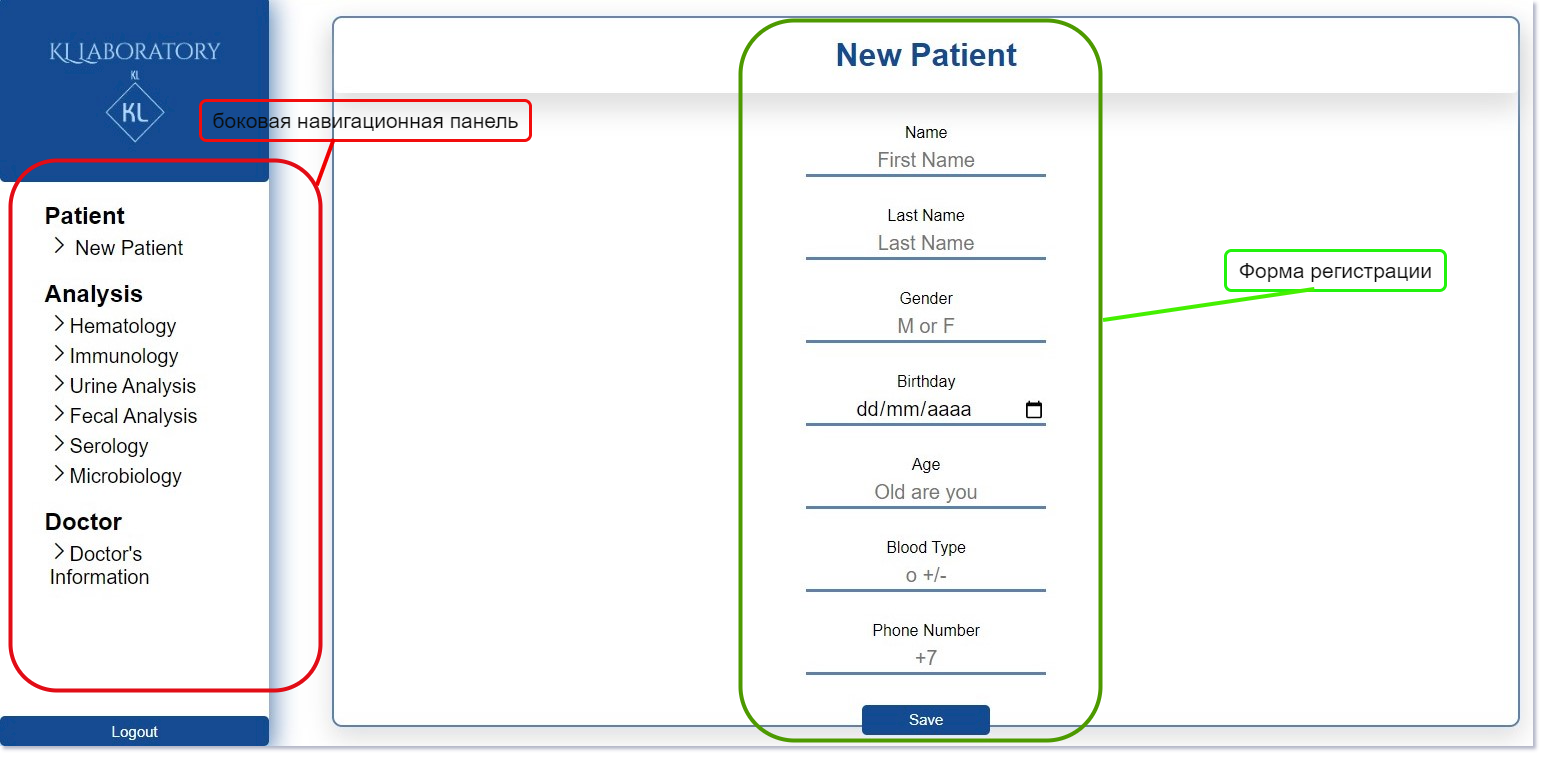
\includegraphics[width=1\linewidth]{pag1}}
\caption{Композиция шаблона сайта}
\label{img:pagp}
\end{figure}

\subsubsection{Исследование предметной области}

Веб-страница в медицинской лаборатории оказывает большую помощь и пользу врачам и персоналу клиники, поскольку служит полезным инструментом для всех процессов, которые они хотят выполнить.
Пользователь должен быть обученным врачом или медсестрой, чтобы правильно ввести данные по каждой процедуре на каждой специализированной форме.
Поля для ввода информации имеют свою собственную связь с базой данных.
В меню врач может перемещаться и выбирать нужную специальность для соответствующей записи. 
Сайт имеет четыре основные функции: сохранение формы, загрузка базы данных пациентов, начало и выход. 

\subsection{Требования к функциональным характеристикам}

\subsubsection{Прецеденты}

Разрабатываемая веб-система предназначена для облегчения управления пациентами и врачами в медицинской лаборатории. На основе изучения конкретного случая было выявлено несколько прецедентов, которые были реализованы на сайте.

Первый прецедент, ``Registration New Patient'', позволяет врачам вводить персональные данные пациентов, приходящих в медицинскую лабораторию. Далее, прецедент ``Save Patient'' используется для проверки и сохранения информации, введенной в форму, и сохранения ее в базе данных системы.

После сохранения данных пациента прецедент ``Choose Analysis'' позволяет врачу или медсестре выбрать тест той специальности, которая необходима пациенту. 

Перед ``Enter Hematology results'' врач или медсестра должны записать все проведенные тесты вместе с результатами для соответствующей проверки врачом и после оценки врачом написать лечение пациента в том же отделе ``Hematology''. Далее используется прецедент ``Save form'', нажав кнопку сохранения, система проверит информацию и сохранит ее в таблице ``Hematology'' в базе данных.

Предшествующая форма ``Enter Immunology Results'' позволяет врачу или медсестре ввести информацию для проведения обследования пациента, следуя полям формы ``Immunology'', таким же образом ввести результаты для соответствующей проверки врача и лечения пациента. После этого прецедента используется прецедент ``Save Form'', когда врач или медсестра хочет сохранить записи в форме ``Immunology'' в базе данных системы.

Прецедент ``Enter Analysis Urine Result'' позволяет врачу или медсестре ввести информацию об исследованиях, анализах и результатах, проведенных у пациента, для соответствующего подтверждения врачом и перехода к назначению соответствующего лечения пациенту. Далее, прецедент ``Save form`` позволяет врачу или медсестре сохранить все данные, введенные в форму, в таблице ``Urine'' в базе данных.

Прецедент ``Enter Fecal Analysis Results'' позволяет врачу или медсестре ввести информацию из всех полей формы по специальности ``Fecal Analysis'', т.е. осмотр, анализ и результаты пациента, для оценки врачом и записи истории болезни и лечения пациента. Далее используется прецедент ``Save form'', позволяющий врачу или медсестре сохранить информацию, введенную в форму ``Fecal Analysis'' для записи на вкладке в базе данных системы.

Прецедент ``Enter Serology Results'' позволяет врачу или медсестре ввести информацию об исследованиях, анализах и результатах, проведенных по специальности для пациента, для соответствующей оценки врачом и лечения пациента. После ввода данных команда ``Save form'' позволяет врачу или медсестре сохранить все введенные в форму данные в резервном файле.

Прецедент ``Enter Microbiology Results'' это позволяет врачу или медсестре вводить информацию, которая предоставляется пациенту, заполняя поля формы ``Microbiology'', а также вводить данные результатов для соответствующей проверки врачом.и лечение, которое необходимо провести пациенту. После этого прецедента продолжается прецедент ``Save form'', который используется, когда врач или медсестра хотят сохранить введенные данные в форме ``Microbiology'' в табе, назначенном для специальности в базе данных системы.

Первый прецедент, ``Registration New Doctor'', позволяет врачу или медсестре вводить личную информацию нового врача, который будет работать в медицинской лаборатории, а также имя пользователя и пароль, назначенные для входа в систему веб-сайта. Далее, предыдущее ``Save Doctor'' используется для проверки и сохранения информации, введенной из формы, и сохранения в базе данных системы.

Наконец, прецедентная ``Information'' позволяет врачу или медсестре проверять и анализировать в таблице всю информацию о пациентах, зарегистрированных в медицинской лаборатории.

Таким образом, использование этих прецедентов на веб-сайте медицинской лаборатории позволяет эффективно управлять пациентами, врачами и специалистами, а также предлагает практическое решение для управления информацией, необходимой в медицинской лаборатории.

Диаграмма приоритетов для программной среды изображена на рисунке \ref{img:usua}.

\begin{figure}
	\center{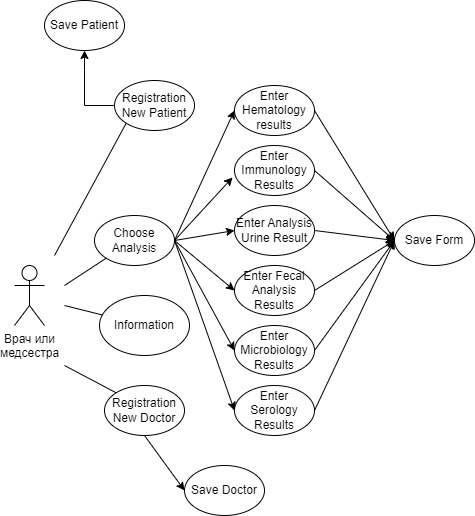
\includegraphics[width=1\linewidth]{diagramauso}}
	\caption{Диаграмма прецедентов}
	\label{img:usua}
\end{figure}

\subsubsection{Сценарии прецедентов программного изделия}

Сценарий для варианта использования "Пользователь и пароль".
Главное действующее лицо: врач или медсестра.
Действующие лица и их требования: врачу или медсестре необходимо будет войти в систему, введя идентификатор пользователя и пароль зарегистрированного врача .
Предварительное условие: наличие подключения к Интернету и должна быть загружена веб-страница медицинской лаборатории.
Последующее условие: После подтверждения врачом идентификатора пользователя и пароля врач или медсестра получат доступ ко всей информации и формам всех специализированных служб, информации о врачах и пациентах медицинской лаборатории.

Основной сценарий успеха:

\begin{enumerate}
	\item Пользователь вводит правильное имя пользователя и пароль.
	\item Пользователь нажимает кнопку ``New Patient''.
	\item Система отображает форму нового пациента.
	\item Пользователь вводит информацию в поля формы.
	\item Пользователь нажимает кнопку ``Save''.
	\item Система записывает всю информацию, введенную в поля формы нового пациента.
	\item Система отображает сообщение об эффективном сохранении.
	\item Пользователь нажимает на меню ``New Doctor''.
	\item Система отображает форму для приема к новому врачу.
	\item Пользователь заполняет поля формы нового врача.
	\item Пользователь нажимает кнопку ``Save''.
	\item Система записывает информацию, внесенную в таблицу врачей, в базу данных.
	\item Система отображает сообщение об эффективности сохранения в системной базе данных.
	\item Пользователь выбирает из меню специальность ``Hematology''.
	\item Система отображает анкету по специальности ``Hematology''.
	\item Пользователь вводит запрашиваемую информацию в специальную форму.
	\item Пользователь нажимает кнопку ``Save''.
	\item Система записывает информацию, внесенную в таблицу ``Hematology'', в базу данных системы.
	\item Система отображает временное сообщение о фактическом сохранении.
	\item Пользователь выбирает из меню специальность ``Immunology''.
	\item Система отображает анкету по специальности ``Immunology''.
	\item Пользователь вводит запрашиваемую информацию в специальную форму.
	\item Пользователь нажимает кнопку ``Save''.
	\item Система записывает информацию, введенную в таблицу ``Immunology'', в базу данных системы.
	\item Система отображает временное сообщение о фактическом сохранении.
	\item Пользователь выбирает из меню специальность ``Urine Analysis''.
	\item Система отображает форму по специальности ``Urine Analysis''.
	\item Пользователь вводит запрашиваемую информацию в специальную форму.
	\item Пользователь нажимает кнопку ``Save''.
	\item Система записывает информацию, введенную в таблицу ``Urine'', в базу данных системы.
	\item Система отображает временное сообщение о фактическом сохранении.
	\item Пользователь выбирает из меню специальность ``Fecal Analysis''.
	\item Система отображает форму по специальности ``Fecal Analysis''.
	\item Пользователь вводит запрашиваемую информацию в специальную форму.
	\item Пользователь нажимает кнопку ``Save''.
	\item Система записывает информацию, введенную в таблицу ``Fecal'', в базу данных системы.
	\item Система отображает временное сообщение о фактическом сохранении.
	\item Пользователь выбирает из меню специальность ``Serology''.
	\item Система отображает анкету по специальности ``Serology''.
	\item Пользователь вводит запрашиваемую информацию в специальную форму.
	\item Пользователь нажимает кнопку ``Save''.
	\item Система записывает информацию, введенную в таблицу ``Serology'', в базу данных системы.
	\item Система отображает временное сообщение о фактическом сохранении.
	\item Пользователь выбирает из меню специальность ``Microbiology''.
	\item Система отображает анкету по специальности ``Microbiology''.
	\item Пользователь вводит запрашиваемую информацию в специальную форму.
	\item Пользователь нажимает кнопку ``Save''.
	\item Система записывает информацию, внесенную в таблицу ``Microbiology'', в базу данных системы.
	\item Система отображает временное сообщение о фактическом сохранении.
	\item Пользователь выбирает из меню специальность ``Information''.
	\item Система отображает таблицу со всей информацией о пациентах, зарегистрированных в медицинской лаборатории.
	\item Пользователь нажимает кнопку выхода.
	\item Вошедший в систему пользователь выходит из системы.
\end{enumerate}

\subsection{Моделирование вариантов использования}

Моделирование сценариев использования - это популярный подход, используемый для понимания функциональных возможностей и требований веб-сайта. В случае медицинской лаборатории варианты использования основаны на потребностях пациентов и лаборатории.

В случае использования веб-сайта медицинской лаборатории врачи должны иметь возможность доступа к подробной информации об услугах, предлагаемых лабораторией, и личной информации о пациентах. Сюда входит информация о проведенных тестах, диагностических услугах и доступных методах лечения. 

Для разрабатываемого сайта была создана модель, которая обеспечивает визуальное представление сценариев использования сайта.
Эта модель помогает как в физической разработке, так и в детальном анализе связей между объектами.
Эта диаграмма представляет собой первоначальную концепцию системы в процессе ее проектирования и разработки и описывает набор действий, которые система предоставляет пользователям, которые являются действующими лицами или сущностями, взаимодействующими с системой.

С учетом анализа темы, в программе должны быть реализованы следующие прецеденты:
\begin{enumerate}
\item Просмотреть информацию о медицинской лаборатории.
\item Просмотр информации о медицинских лабораторных процессах.
\item Посмотреть информацию об услугах медицинской лаборатории.
\item Просмотреть реестр информации врачей и пациентов.
\item Поиск результатов.
\end{enumerate}

\subsection{Требования к обработке баз данных}

В медицинской лаборатории важно, чтобы на сайте была база данных для управления медицинскими данными пациентов и документацией, связанной с медицинскими услугами. Эта база данных должна быть безопасной и соответствовать всем нормам конфиденциальности и информационной безопасности.

Важно, чтобы в базе данных можно было осуществлять поиск и фильтрацию, чтобы сотрудники лаборатории могли искать медицинскую информацию по конкретным пациентам. База данных может предоставлять ограниченный доступ к личным и медицинским данным только уполномоченному медицинскому персоналу.

База данных может позволять регулярно обновлять медицинские данные пациентов уполномоченным медицинским персоналом. Кроме того, она может обеспечивать доступ к результатам лабораторных анализов в режиме реального времени.

В качестве дополнительного важного требования база данных имеет возможность генерировать отчеты и статистику на основе хранящихся данных. Это позволит врачам и сотрудникам медицинских лабораторий получить доступ к полезной информации, которая поможет в диагностике и лечении пациентов.

Процесс установки и использования систем управления базами данных может быть сложным. Для использования программного обеспечения управления данными в медицинской лаборатории необходимо подключение к Интернету и компьютер с установленным языком программирования MYSQL. Информация вводится в систему с помощью клавиатуры и мыши путем заполнения необходимых полей.
Каждый врач имеет уникальное имя пользователя, которое дает ему доступ ко всем функциям системы. Для обеспечения правильного хранения информации о госпитализации и лечении пациентов важно, чтобы врачи умели писать последовательно и четко.
Система должна иметь возможность хранить соответствующую информацию о результатах анализов, проведенных пациентам. У каждого врача и каждого пациента в системе может быть записано несколько анализов. Кроме того, система может осуществлять поиск и запрос конкретной информации о пациентах и результатах анализов.
В целом, системы управления базами данных являются необходимыми инструментами для управления медицинской информацией в лаборатории. В целом, системы управления базами данных являются необходимыми инструментами для управления медицинской информацией в лаборатории.
Хотя они могут быть сложными в установке и использовании, они необходимы для обеспечения эффективного управления информацией о пациентах. для обеспечения эффективного управления информацией о пациентах.

\subsection{Требования к информации и совместимости веб-приложения}

В медицинской лаборатории веб-сайт играет важную роль в предоставлении информации, повышении эффективности процессов и улучшении качества медицинских услуг. Важно, чтобы веб-сайт медицинской лаборатории предоставлял четкую и точную информацию о предлагаемых ею медицинских услугах. 

Веб-сайт совместим с различными браузерами и операционными системами, которыми располагает медицинская лаборатория, чтобы обеспечить его доступность для всех врачей. Кроме того, он прост в навигации и использовании, с удобным и интуитивно понятным интерфейсом.

Разрабатываемое веб-приложение имеет простой в использовании и понятный интерфейс для всех врачей, желающих зарегистрировать информацию, выбирая действия, которые они хотят выполнить, такие как регистрация новых пациентов, врачей или заполнение форм специализации.  Пользователи-врачи будут рассматриваться как главные пользователи, которые будут иметь доступ ко всей информации на сайте медицинской лаборатории. 
Для разработки среды веб-сайта необходимо использовать:

\begin{itemize}
	\item xampp - для подключения кода к веб-браузеру.
	\item Требуется подключение к Интернету.
	\item Требуется подключение к базе данных MySQL.
\end{itemize}

Совместимость веб-сайта медицинской лаборатории - это способность правильно функционировать с различными устройствами и веб-браузерами, а также обеспечивать плавный и эффективный просмотр сайта для пользователей, особенно для пациентов.
Сайт совместим с различными веб-браузерами, такими как Chrome, Firefox, Safari, Opera, Internet Explorer и т.д., сайт также адаптируется к различным размерам экрана, от настольных компьютеров до мобильных устройств, таких как телефоны и планшеты.
Сайт быстро загружается и обеспечивает хороший пользовательский опыт, с простой и доступной навигацией и четким и лаконичным содержанием, сайт соответствует правилам и нормам, относящимся к медицинскому сектору и защите данных пациентов.
Сайт легко доступен и удобен для использования врачами разных специальностей и уровней квалификации.
Врач будет использовать клавиатуру в качестве метода ввода и компьютерную мышь для выбора. О любых ошибках, допущенных врачом или при вводе данных в режиме онлайн, система будет сообщать предупреждающим сообщением с указанием места и причины ошибки. Продукт веб-приложения должен работать на операционных системах Windows с установленными Sun JDK 1.1.8, Microsoft SDK 3.1, IBM JDK 1.1.7B или более поздней версии. Требуется наличие Visual Studio Code и MYSQL.

\subsubsection{Требования к надежности}

При проектировании и разработке веб-сайта медицинской лаборатории были соблюдены определенные требования к надежности, чтобы обеспечить положительный опыт пользователей и защиту информации о пациентах. Эти требования включают:

\begin{enumerate}
	\item Информационная безопасность: На сайте предусмотрены меры безопасности для обеспечения конфиденциальности и защиты данных пациентов. Проактивный подход в предотвращении нарушений безопасности, поскольку медицинская информация является конфиденциальной и должна быть защищена от несанкционированного доступа третьих лиц.
	\item Достоверная информация: Информация, представленная на сайте, должна быть точной и надежной. Убедитесь, что информация актуальна и отражает услуги и процедуры, предлагаемые в медицинской лаборатории на данный момент, а также результаты.
	\item Функциональность: веб-сайт должен обладать эффективной и бесперебойной функциональностью для клиницистов. Это включает в себя быстрое время загрузки, простую навигацию и четкий, удобный для пользователя дизайн.
	\item Частое обновление: Важно, чтобы веб-сайт медицинской лаборатории часто обновлялся, чтобы отражать изменения в предоставляемых услугах и выполняемых процедурах.
	\item Техническая поддержка: на сайте имеется техническая поддержка, обеспечивающая своевременное решение любых технических проблем.
\end{enumerate}

Веб-приложение должно работать во всех разработанных тестах. Тесты должны быть разработаны 
на этапе детального проектирования.

\subsubsection{Условия эксплуатации}

В операционной среде веб-сайта для медицинской лаборатории были приняты во внимание следующие элементы для обеспечения эффективности, безопасности и надежности веб-сайта:

\begin{enumerate}
	\item Серверы базы данных: формы на веб-сайте подключены к базе данных. База данных имеет соответствующие средства защиты для хранения введенной информации.
	\item Пропускная способность: достаточная пропускная способность считается важной для обеспечения быстрой загрузки сайта и предотвращения потери данных.
	\item Обновления и обслуживание: веб-сайт должен надлежащим образом обновляться и обслуживаться, чтобы избежать ошибок, технических проблем или потери информации.
	\item Операционные системы: веб-сайт совместим с большинством операционных систем для их соответствующего функционирования.
	\item Платформа для разработки веб-сайта: в качестве платформы для разработки веб-сайта была выбрана Visual Studio Code.
	\item Информационная безопасность: веб-сайт имеет проверку пользователей и паролей для обеспечения защиты информации, включенной в него.
\end{enumerate}

\subsection{Требования к оформлению документации}

Разработка программной документации и программного изделия должна производиться согласно ГОСТ 19.102-77 и ГОСТ 34.601-90. Единая система программной документации.

\subsection{Стадии и этапы разработки}

Разработка веб-страницы для медицинской лаборатории проводилась в три этапа: техническое задание, технический проект и проект реализации. На этапе технического задания с помощью обзора литературы были определены необходимые требования к веб-странице, и был составлен документ ``техническое задание''. На этапе технического проекта был проведен тщательный анализ темы и была разработана структура программы. Наконец, на стадии рабочего проекта была разработана функциональная реализация веб-сайта, включая тестирование и оценку. Результаты каждого этапа были оформлены в документах ``технический проект'' и``рабочий проект''.
	\newsection
\section{Технический проект}
\subsection{Общая характеристика организации решения задачи}

Планирование и создание веб-сайта необходимо для того, чтобы оптимизировать способ хранения и организации информации в медицинской лаборатории.

Веб-сайт - это набор веб-страниц, размещенных на сервере и связанных между собой. Каждая веб-страница содержит информацию, которая может быть представлена в различных форматах, таких как текст, изображения и видео, среди прочих. Эти веб-сайты создаются с определенной целью, будь то информирование, продвижение товаров или услуг, предоставление развлечений и т.д. Создание веб-сайта включает в себя планирование, проектирование и разработку логической структуры для представления информации в Интернете с целью облегчения доступа и удобства для пользователей\cite{website}.

Веб-сайт может иметь и другие элементы, такие как контактные формы, системы внутреннего поиска, ссылки на другие веб-сайты, кнопки для обмена контентом в социальных сетях, а также другие элементы, направленные на улучшение производительности и функциональности сайта.

Существуют также различные типы веб-сайтов, от личных страниц и блогов до интернет-магазинов и корпоративных сайтов. Каждый тип веб-сайта имеет свои специфические характеристики и цели.

Процесс создания веб-сайта включает в себя выбор платформы или языка программирования, выбор веб-хоста, приобретение доменного имени, создание контента и графического дизайна. Также важно учитывать использование методов SEO (поисковой оптимизации), чтобы сделать сайт видимым в результатах поиска поисковых систем.

Общая организация веб-сайта медицинской лаборатории зависит от конкретного содержания, которое вы хотите представить, и цели, которую вы хотите достичь. Ниже перечислены некоторые разделы веб-сайта медицинской лаборатории:

\begin{enumerate}
	\item Главная страница: страница приветствия, на которой есть поля для входа в систему и ввода пароля врача.
	\item Услуги: навигационный раздел, в котором перечислены предлагаемые услуги, такие как анализы крови, медицинские анализы и другие медицинские услуги.
	\item Формы: раздел для заполнения личных данных пациента, а также записей о его лечении, наблюдении, приеме лекарств и анализах с помощью формы с обязательными и необязательными полями.
	\item Результаты: раздел, в котором врачи могут получить доступ к результатам лабораторных анализов в режиме онлайн в безопасной и эффективной системе.
	\item Навигационные таблицы: включает навигационную таблицу для поиска ранее зарегистрированных пациентов.
\end{enumerate}

медицинская лаборатория уникальна, поэтому разделы продумываются исходя из конкретных целей и потребностей. Сайт интуитивно понятен и предлагает клиницисту оптимальную навигацию для поиска актуальной и полезной информации о пациенте.

\subsubsection{Словарь предметной области продукта веб-странице изделия}

Тщательный анализ предметной области был проведен в технической спецификации, а термины на английском и испанском языках были собраны в словаре по предметной области. Этот словарь основан на разделе № 2 технической спецификации. С другой стороны, в таблице \ref{table:dic} представлен словарь данных среды разрабатываемой веб-страницы, отвечающий за выполнение всех услуг, предлагаемых веб-страницей для медицинской лаборатории.


\begin{xltabular}{\textwidth}{|p{4cm}|p{12cm}|}
	\caption{Словарь данных для части среды разрабатываемой веб-страницы.\label{table:dic}}\\ \hline
	\thead{Термин} & \thead{Описание} \\ \hline
	\thead{1} & \thead{2} \\ \hline
	\endfirsthead
	\continuecaption{Продолжение таблицы \ref{table:dic}}
	\thead{1} & \thead{2} \\ \hline
	\finishhead
	Поле«интерфейс входа в систему» & Это главная страница, на которой будут подтверждены логин и пароль врача \\ \hline 
	Поле«форма для пациентов» & После подтверждения имени пользователя и пароля, введенного непосредственно в форму для регистрации нового пациента, здесь пользователь должен заполнить поля в форуме, если он хочет ввести нового пациента. \\ \hline 
	Поле«специальная форма» & В зависимости от специальности, выбранной врачом или медсестрой, будет развернута форма специальности.  \\ \hline 
	Поле«форма нового врача» & Пользователь сможет ввести личные данные нового врача, который будет работать в медицинской лаборатории, и указать имя пользователя и пароль.  \\ \hline 
	Поле«информация о пациентах» & Врач или медсестра смогут просмотреть в таблице все данные о пациентах, поступивших в медицинскую лабораторию. \\ \hline 
	Поле«выход из системы» & При заполнении этого поля система закроет начатый сеанс врача.  \\ \hline 
\end{xltabular}

\subsection{Обоснование выбора технологии проектирования}

Использование веб-сайта в медицинской лаборатории оправдано по нескольким причинам. Веб-сайт поможет улучшить организацию и учет информации, облегчая доступ к данным в режиме онлайн. Он также может служить платформой для передачи соответствующей информации врачам. Кроме того, веб-сайт обеспечивает безопасность только для сотрудников, обученных работе с личной информацией пациентов, проведенными тестами, лечением и результатами. Веб-сайт также может использоваться для регистрации данных о врачах с указанием их специальностей и номеров кабинетов, где они находятся.

В настоящее время длительные процессы можно решить с помощью собственного программного обеспечения, поскольку хорошая поддержка мультимедиа HTML способна легко интегрировать мультимедийные элементы, такие как изображения, видео и аудио, в веб-страницу, что выгодно, когда вы хотите обеспечить разнообразие в контенте.

Гибкость дизайна HTML как языка разметки позволяет дизайнерам создавать индивидуальные стили и макеты страниц, предоставляя разработчикам полный контроль над визуальным оформлением веб-страниц.

\subsubsection{Описание используемых технологий и языков программирования}

При создании веб-сайта используются различные программные инструменты и языки программирования, каждый из которых применяется в зависимости от различных задач, которые необходимо выполнить.

HTML - одна из основополагающих технологий в веб-программировании. HTML используется для определения структуры и содержания веб-страницы, то есть элементов, из которых она состоит, и их иерархической организации.
В дополнение к HTML существуют и другие технологии, такие как CSS, которые позволяют определять стили и визуальное форматирование веб-страницы.
HTML был разработан в начале 1990-х годов и с течением времени развивался, включая новые функции и возможности. Совет Всемирной паутины (W3C) является организацией, ответственной за разработку и поддержание стандартов HTML.
Навыки, необходимые для изучения HTML, включают понимание тегов, базовой структуры веб-страниц, атрибутов, ссылок, форм, а также использование изображений и видео.
В целом, HTML - это важный язык разметки, используемый для разработки современных веб-страниц и являющийся фундаментальным компонентом веб-программирования.
HTML используется для создания структурированного веб-контента. 
HTML-теги позволяют организовать содержимое веб-страницы в различные разделы, такие как заголовки, абзацы, таблицы, изображения, формы и ссылки. медицинские лаборатории могут использовать эти теги, чтобы сделать свою информацию легко читаемой и доступной для клиницистов.
Оформление и внешний вид веб-сайта также должны соответствовать медицинскому имиджу лаборатории. Поэтому была использована соответствующая цветовая схема и обеспечено профессиональное и четкое представление контента.

\subsubsection{Язык программирования PHP}

PHP использовался на сайте для разработки системы управления пациентами, в которой хранится информация о пациентах и упорядочивается администрирование и организация медицинских услуг лаборатории. Он также использовался для автоматизации обработки и анализа медицинских данных, создания отчетов и интеграции с другими медицинскими информационными системами. PHP способен взаимодействовать с базами данных, что выгодно для записи, запроса и поиска информации быстро и эффективно\cite{php2}.
PHP имеет такие фреймворки, как Laravel и Symfony, которые делают его очень мощным и профессиональным. Важно отметить, что PHP является объектно-ориентированным языком, что позволяет использовать его для решения множества задач программирования. Он также имеет большое сообщество, что гарантирует постоянную поддержку и регулярные обновления языка\cite{php1}. 

PHP имеет C-подобный синтаксис и предназначен для взаимодействия с базами данных и доставки динамического содержимого через Интернет с помощью технологии веб-сервера. Некоторые из наиболее заметных особенностей PHP следующие:

\begin{enumerate}
	\item Интерпретация: исходный код PHP выполняется на сервере перед отправкой страницы в браузер пользователя.
	\item Простая интеграция с HTML: PHP позволяет внедрять PHP-код внутрь HTML-страниц для создания динамических веб-страниц.
	\item Подключение к базе данных: PHP имеет широкий спектр расширений для подключения к базам данных, что облегчает разработку приложений, использующих базы данных.
	\item Объектно-ориентированный: PHP также поддерживает объектно-ориентированное программирование.
	\item Обширная документация и сообщество: PHP имеет обширную документацию и активное онлайн-сообщество пользователей, которые предлагают поддержку и ресурсы для разработки на этой технологии.
\end{enumerate}

PHP работает на сервере и генерирует HTML, который отправляется в браузер пользователя для отображения. Помимо HTML, PHP может генери ровать и другие типы контента, такие как изображения и PDF-файлы.
Использование PHP на сайте медицинской лаборатории полезно, поскольку это язык программирования, позволяющий создавать динамический контент на сайте. PHP использовался для создания интерактивных форм, автоматизации онлайн-задач, интеграции баз данных и защиты информации о пациентах.
В медицинской лаборатории PHP может быть использован для создания страницы с интерактивными формами, позволяющими врачам регистрироваться и получать информацию в автоматическом режиме.
PHP имеет множество функций безопасности для защиты целостности данных пациентов, что делает его хорошим выбором для медицинской среды.

\subsubsection{Преимущества языка PHP}

Существует несколько преимуществ использования PHP для разработки веб-сайта, например, следующие:

\begin{enumerate}
	\item Легкость изучения: PHP считается одним из самых простых языков для изучения, что делает его популярным среди начинающих разработчиков.
	\item Доступность на различных платформах: PHP работает на различных операционных системах, что делает его гибким и универсальным.
	\item Интеграция с MySQL: Используя PHP в сочетании с MySQL, вы получаете доступ к широким возможностям работы с данными и их обработки.
	\item Большое и опытное сообщество: Существует большое сообщество разработчиков и пользователей PHP по всему миру, которые делятся своими знаниями и ресурсами, что облегчает процесс обучения и устранения неполадок.
	\item Скорость выполнения: PHP предлагает быстрое и эффективное выполнение по сравнению с другими языками программирования.
	\item Персонализация: PHP очень легко настраивается и адаптируется к различным потребностям и специфическим требованиям проектов веб-разработки.
\end{enumerate}

\subsubsection{Недостатки языка PHP}

К недостаткам использования PHP на веб-странице можно отнести следующие:

\begin{enumerate}
	\item Проблемы безопасности: При неправильной настройке использование PHP на веб-странице может вызвать проблемы с безопасностью, поскольку этот язык позволяет выполнять код на сервере.
	\item Необходимость в веб-сервере: Для того чтобы веб-страница могла выполнять код PHP, требуется веб-сервер, что может увеличить расходы на хостинг и обслуживание.
	\item Ограниченная масштабируемость: По мере роста и усложнения веб-сайта производительность PHP может быть ограничена.
	\item Сложная отладка: При работе с PHP-кодом может быть трудно отлаживать специфические ошибки и проблемы из-за сложности языка.
	\item Избыточный код: PHP может генерировать громоздкий код на веб-страницах, что может замедлить скорость загрузки и негативно повлиять на пользовательское восприятие.
\end{enumerate}

\subsection{Язык стилей CSS}

Использование CSS на сайте медицинской лаборатории определило визуальное представление и стиль сайта, что помогает улучшить опыт врача и облегчает понимание информации, представленной на сайте. В целом, CSS помогает улучшить представление и читабельность информации на странице, что может быть полезно в условиях, когда важно представить медицинскую информацию четко и точно.

Таблицы стилей CSS содержат правила, определяющие стиль элементов HTML, к которым они применяются\cite{css1}. Каждое правило состоит из селектора, указывающего элементы, к которым будет применен стиль, и набора свойств, определяющих стиль элемента. Свойства могут включать цвет фона, шрифт, размер шрифта, межстрочный интервал, размер границы и другие.

\subsubsection{Достоинства языка CSS}

К преимуществам языка стилей CSS относятся:

\begin{enumerate}
	\item Разделение содержания и представления, что облегчает обслуживание и модификацию сайта.
	\item Эффективность загрузки страницы, поскольку стили могут быть определены и применены к различным элементам.
	\item Гибкость дизайна, поскольку настраиваемые стили могут применяться и адаптироваться к различным устройствам и разрешениям.
	\item Простота использования, поскольку это декларативный язык, а его синтаксис интуитивно понятен и прост для понимания.
	\item Он позволяет создавать целостный дизайн всего сайта, что повышает удобство использования и улучшает впечатления пользователей.
\end{enumerate}

\subsubsection{Недостатки языка CSS}

К возможным недостаткам языка стилей CSS относятся следующие:
\begin{enumerate}
	\item Сложность обучения правильному использованию, особенно для дизайнеров, которые привыкли использовать графические инструменты для создания дизайна.
	\item Возможна несовместимость между различными браузерами и версиями, что может потребовать дополнительного тестирования и корректировки стилей для обеспечения совместимости.
	\item Поскольку это универсальный и гибкий инструмент, могут возникнуть проблемы с производительностью, если применяется слишком много сложных стилей или они не оптимизированы должным образом.
	\item Для выполнения некоторых сложных задач CSS могут потребоваться дополнительные навыки программирования.
\end{enumerate}

В целом, однако, преимущества CSS значительно превосходят потенциальные недостатки, и он зарекомендовал себя как ключевой элемент эффективного дизайна современных веб-сайтов.

\subsection{Диаграмма компонентов и схема обмена данными между файлами компонента}

Диаграммы компонентов полезны в программировании, поскольку они дают общее представление о системе и определяют взаимосвязи между различными компонентами, что облегчает понимание и сопровождение кода и может помочь выявить потенциальные проблемы и улучшения в системе. Кроме того, диаграммы компонентов могут служить основой для построения архитектуры программного обеспечения и планирования его развития.

На рисунке \ref{image:diagram} показана компонентная диаграмма работы сайта.

\begin{figure}
\centering{\includegraphics[width=1\linewidth]{diagramadecomponentes}}
\caption{Диаграмма компонентов}
\label{image:diagram}
\end{figure}

Вызов любого компонента на веб-странице требует, чтобы он был включен в код сценария соответствующей страницы. При вызове компонента происходит передача данных от страницы к соответствующему компоненту.

На рисунке \ref{image:diagram2} показано, как происходит обмен данными между скриптами компонента и веб-страницей при вызове компонента.

\begin{figure}
\centering{\includegraphics[width=0.5\linewidth]{diagramacomp2}}
\caption{Схема обмена данными между веб-страницей и скриптом}
\label{image:diagram2}
\end{figure}

Сценарий веб-страницы устанавливает значения параметров компонента во время вызова, которые затем передаются сценарию в файле index.php.
В скрипте файла index.php метод session\_stat с помощью метода\linebreak if(isset(isset(\$SEASION['user\_id']))) вызывает компонент login.php, в котором будет проверен пользователь, желающий войти на платформу сайта. Идентификатор врача будет авторизован для доступа ко всем функциям сайта.\linebreak После эффективного входа подключается скрипт файла Patient.php одного из шаблонов, который представлен формой для регистрации персональных данных каждого пациента. С помощью компонента nav.html врач может выбрать варианты навигационного меню сайта. Если в меню будет выбран пункт ``Doctors'', то будет вызван скрипт doctors.php - шаблон, в котором будет отображена форма для ввода персональных данных врачей, работающих в медицинской лаборатории. Аналогично, если будет выбран пункт ``Analysis'', то будет вызван скрипт каждой нужной специальности и отображена форма для регистрации каждого пациента по специальности. 

Операции скрипта и все, что зарегистрировано из форм, вызовут метод Conexion.php, который осуществит соединение с базой данных, и произведет консультацию, сохранение и удаление информации в базе данных.

\subsection{Диаграмма развертывания}

Диаграмма размещения (рис.~\ref{image:diagram3}) представляет физические взаимодействия, существующие между аппаратными и программными частями анализируемой системы.

\begin{figure}
\centering{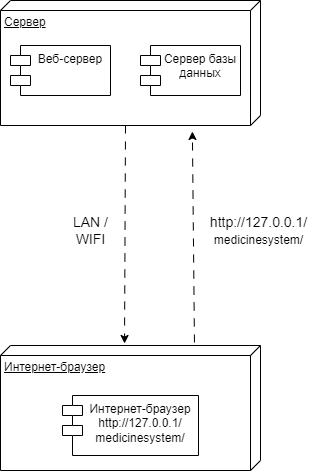
\includegraphics[width=0.37\linewidth]{diagramacomp3}}
\caption{Диаграмма развертывания}
\label{image:diagram3}
\end{figure}

Диаграмма размещения показывает представление физических взаимодействий между аппаратными и программными частями системы веб-сайта с серверами.

\subsection{Схема базы данных}

Диаграммы таблиц MySQL - полезный инструмент для визуализации структуры базы данных и связей между ее таблицами, поскольку они облегчают понимание структуры базы данных. Представление базы данных MySQL покажет реализацию и архитектуру таблиц для данных о специальности, враче и пациенте медицинской лаборатории.
Диаграмма на \ref{image:base} показывает мертвые таблицы, созданные в MySQL.

База данных может быть полезна для управления данными в медицинской лаборатории. медицинские лаборатории производят большое количество данных о пациентах, включая информацию о лабораторных тестах и другую медицинскую информацию. База данных в медицинской лаборатории включает в себя:

\begin{enumerate}
	\item Хранение информации о пациенте и истории болезни.
	\item Хранение информации о проведенных лабораторных тестах и полученных результатах.
	\item Выявление закономерностей в данных для идентификации типов пациентов и результатов лабораторных тестов.
	\item Формирование отчетов о результатах лабораторных исследований для обеспечения лечения пациента.
	\item Повышение качества данных и сокращение количества ошибок путем проверки данных и выявления ошибок перед сохранением данных в базе данных.
\end{enumerate}

\begin{figure}
	\centering{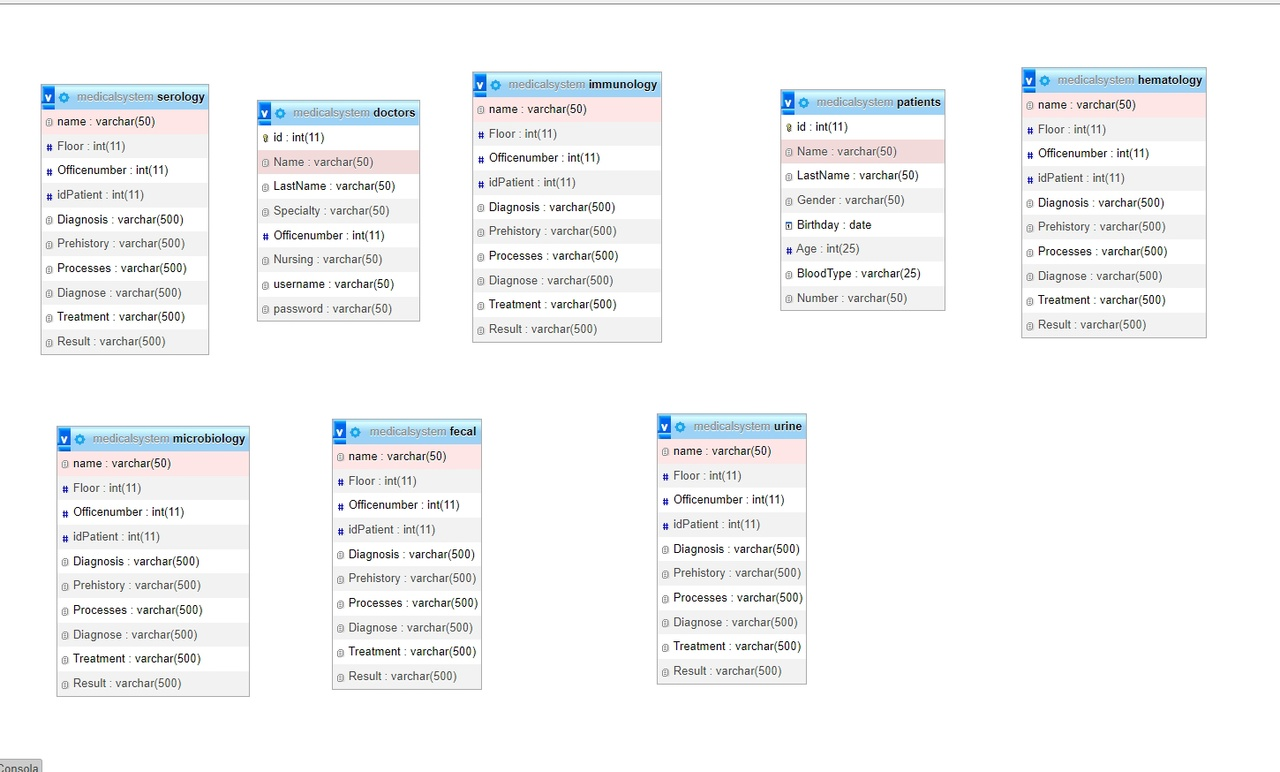
\includegraphics[width=1\linewidth]{base}}
	\caption{Схема базы данных}
	\label{image:base}
\end{figure}

\subsection{Содержание форм на веб-сайте}

Веб-сайт медицинской лаборатории играет ключевую роль в общении с врачами, предоставляя важную информацию о предоставляемых услугах и результатах. Одним из наиболее важных аспектов веб-сайта медицинской лаборатории является содержание форм, представленных на сайте. Эти формы должны быть четкими, полными и эффективными, чтобы обеспечить удовлетворительный опыт для врачей.

Во-первых, онлайн-формы легко найти и выбрать на сайте медицинской лаборатории, а четкая и интуитивно понятная структура позволяет врачам быстро найти и заполнить формы. Кроме того, формы адаптируемы, так что их можно читать и заполнять на любом компьютере, без потери качества и удобства использования.

Во-вторых, бланки имеют хорошую организацию и структуру, с четкими инструкциями по каждому из разделов. 

В-третьих, бланки медицинской лаборатории безопасны. Пациенты должны быть уверены, что информация, которую они предоставляют в бланках, будет обрабатываться конфиденциально и безопасно. На сайте предусмотрены адекватные меры безопасности для защиты личной и медицинской информации, собранной в бланках.

Наконец, важно, чтобы лаборатория постоянно обновляла бланки, предоставляя последнюю информацию о выполненных для пациентов услугах, обеспечивая точность и актуальность бланков для врачей.

Формы на сайте, состоящие из обязательных и необязательных полей, основаны на следующих трех структурах:

\begin{itemize}
\item "<Doctors">;
\item "<Patient">;
\item "<Analysis">.
\end{itemize}

В форме "<Doctors"> содержит поля, показанные в следующей таблице \ref{table:doctors}.

\begin{xltabular}{\textwidth}{|l|l|p{1.7cm}|X|}
	\caption{Форме "<Doctors">\label{table:doctors}}\\ \hline
	\thead{Поле} & \thead{Тип} & \thead{Обяза-\\тельное} & \thead{Описание} \\ \hline
	\thead{1} & \thead{2} & \thead{3} & \thead{4} \\ \hline
	\endfirsthead
	\continuecaption{Продолжение таблицы \ref{table:doctors}}
	\thead{1} & \thead{2} & \thead{3} & \thead{4} \\ \hline
	\finishhead
	id & int & true & Идентификатор врача \\ \hline 
	Name & varchar(50) & true & Имя врача \\ \hline 
	LastName & varchar(50) & true & Фамилия врача \\ \hline 
	Specialty & varchar(50) & true & Специальность врача \\ \hline 
	Officenumber & int & false & Офис, где работает врач \\ \hline 
	Nursing & varchar(50) & true & ФИО медсестры \\ \hline 
	username & varchar(50) & true & Пользователь для входа в систему \\ \hline
	password & varchar(50) & true & Пароль врача для входа в систему \\ \hline
\end{xltabular}

Для формы "<Patient"> поля описаны в следующей таблице \ref{table:patient}.


\begin{xltabular}{\textwidth}{|l|l|p{1.7cm}|X|}
	\caption{Форме "<Patient">\label{table:patient}}\\ \hline
	\thead{Поле} & \thead{Тип} & \thead{Обяза-\\тельное} & \thead{Описание} \\ \hline
	\thead{1} & \thead{2} & \thead{3} & \thead{4} \\ \hline
	\endfirsthead
	\continuecaption{Продолжение таблицы \ref{table:patient}}
	\thead{1} & \thead{2} & \thead{3} & \thead{4} \\ \hline
	\finishhead
	id & int & true & Идентификатор пациента \\ \hline 
	Name & varchar(50) & true & Имя пациента \\ \hline 
	LastName & varchar(50) & true & Фамилия пациента \\ \hline 
	Gender & varchar(50) & true & Пол пациента \\ \hline 
	Birthday & date & true & Дата рождения пациента \\ \hline 
	Age & int & true & Возраст пациента \\ \hline 
	BloodType & varchar(25) & true & Определение группы крови пациента \\ \hline
	Number & varchar(50) & false & Контактный номер пациента \\ \hline
\end{xltabular}

В форме "<Analysis"> одна и та же форма используется для всех специальностей медицинской лаборатории и содержит поля, показанные в следующей таблице\ref{table:anali}.

\begin{xltabular}{\textwidth}{|l|l|p{1.7cm}|X|}
	\caption{Форме "<Analysis">\label{table:anali}}\\ \hline
	\thead{Поле} & \thead{Тип} & \thead{Обяза-\\тельное} & \thead{Описание} \\ \hline
	\thead{1} & \thead{2} & \thead{3} & \thead{4} \\ \hline
	\endfirsthead
	\continuecaption{Продолжение таблицы \ref{table:anali}}
	\thead{1} & \thead{2} & \thead{3} & \thead{4} \\ \hline
	\finishhead
	name & varchar(50) & true & ФИО врача-специалиста \\ \hline 
	Floor & int & false & Этаж здания, где находится специальность \\ \hline 
	idPatient & int & true & ФИО пациента \\ \hline 
	Diagnosis & varchar(500) & true & Диагноз пациента \\ \hline 
	Prehistory & varchar(500) & true & История болезни пациента \\ \hline 
	Processes & varchar(500) & true & Процедуры, проводимые с пациентом \\ \hline 
	Diagnose & varchar(500) & true & Текущий диагноз пациента \\ \hline
	Treatment & varchar(500) & true & Лечение пациента \\ \hline
	Result & varchar(500) & true & Результат процессов, проведенных с пациентом \\ \hline
\end{xltabular}

В большинство полей формы ``Analysis'' разрешается вводить текст объемом до 500 символов. История болезни каждого пациента будет уникальна и будет связана с именем пациента, а также с врачом, который проводил процессы у пациента.
Разработанная база данных помогает медицинской лаборатории эффективно хранить, организовывать и управлять данными о пациентах и аналитическими данными, что способствует повышению качества ее данных и созданию точных и полезных отчетов.

\subsection{Моделирование прецедентов}

Для моделирования вариантов использования веб-страницы для медицинской лаборатории в качестве важной части процесса разработки были предоставлены варианты использования, которые помогают определить требования и функциональные возможности веб-страницы и позволяют понять, как пользователи будут взаимодействовать со страницей.

Чтобы смоделировать варианты использования веб-страницы, были предприняты следующие шаги:

\begin{enumerate}
	\item Определение требований: на этом первом этапе были определены необходимые требования, которым должен соответствовать веб-сайт медицинской лаборатории. Это включало понимание потребностей и ожиданий конечного пользователя.
	\item Идентификация субъектов: были определены основные субъекты, которые будут взаимодействовать с веб-страницей, что помогло определить объем и сложность вариантов использования.
	\item Идентификация вариантов использования: на основе выявленных требований и действующих лиц можно было определить необходимые варианты использования для веб-страницы. Эти варианты использования включали такие задачи, как регистрация пациентов, регистрация врачей, регистрация анализов и просмотр результатов тестов.
\end{enumerate}

Описание функций, используемых системой на веб-сайте.
Работа системы состоит из трех основных функций. Эти характеристики описаны ниже.
Имя функции: session\_start();
Предварительное условие: ввод действительных данных пользователя и пароля.
Последующее условие: вызывает функцию Connection, в которой пользователь проверяется на соответствие данным, записанным в базе данных.
Описание функции session\_start(): эта функция при вызове подключения к базе данных проверяет имя пользователя и пароль с данными врачей в базе данных.

Название функции: подключение.
Предварительное условие: система автоматически вводит данные с веб-страницы.
Последующее условие: система ищет таблицу формулы, выбранной пользователем.
Описание функции подключение: это линия подключения к базе данных и таблицам для соответствующей записи введенных данных о новых врачах, пациентах и специальностях по выбору пользователя.

Название функции: сохранить.
Предварительное условие: пользователь заполняет поля используемой формы.
Последующее условие: система записывает то, что было введено через поля шаблона.
Описание функции сохранения: функция выполняет проверку достоверной информации в соответствии с правилами, содержащимися в каждой таблице базы данных, чтобы продолжить соответствующую регистрацию и сохранение введенного пользователем.
	\newsection
\section{Рабочий проект}
\subsection{Модули, используемые при разработке сайта}

Интерфейс для врача или медсестры состоит из следующих компонентов

\begin{itemize}
	\item главное окно входа в систему;
	\item окно для регистрации нового пациента;
	\item форма регистрации нового пациента;
	\item форма регистрации нового врача;
	\item регистрационная форма для специальности ``Hematology'';
	\item регистрационная форма для специальности ``Immunology'';
	\item регистрационная форма для специальности ``Urine Analysis'';
	\item регистрационная форма по специальности ``Fecal Analysis'';
	\item регистрационная форма по специальности ``Serology'';
	\item регистрационная форма по специальности ``Microbiology''.
\end{itemize}

Модули классифицируются на формы, соединения и ввод базы данных.
В таблице \ref{table:modd} описаны модули и функции для формы врача.

\begin{xltabular}{\textwidth}{|p{2.5cm}|p{2.5cm}|p{4.85cm}|p{4.85cm}|}
\caption{Спецификация модуля ``Doctors''.\label{table:modd}}\\
\hline \centrow Название класса & \centrow Модуль, к которому относится класс & \centrow Описание класса & \centrow Методы \\
\hline \centrow 1 & \centrow 2 & \centrow 3 & \centrow 4\\
\endfirsthead
\caption*{Продолжение таблицы \ref{table:modd}}\\
\hline \centrow 1 & \centrow 2 & \centrow 3 & \centrow 4\\
\finishhead
\hline
cont\_form & doctors.php & cont\_form - для создания нового медицинского учреждения, и с необходимыми разрешениями для входа в систему сайта, вместе с методом post для чтения того, что написано в форме. & <class="cont\_form"> <class="head"> <h1>NewDoctror</h1> <method\=``post'' action=``/admin/ Save\_d.php''> \\ \hline
\end{xltabular}

В таблице \ref{table:modp} описывает модули и функции формы пациента.

\begin{xltabular}{\textwidth}{|p{2.5cm}|p{2.5cm}|p{4.85cm}|p{4.85cm}|}
\caption{Спецификация модуля ``Patient''.\label{table:modp}}\\
\hline \centrow Название класса & \centrow Модуль, к которому относится класс & \centrow Описание класса & \centrow Методы \\
\hline \centrow 1 & \centrow 2 & \centrow 3 & \centrow 4\\
\endfirsthead
\caption*{Продолжение таблицы \ref{table:modp}}\\
\hline \centrow 1 & \centrow 2 & \centrow 3 & \centrow 4\\
\finishhead
\hline
cont\_form & Patient.php & cont\_form -  помогает создать новую запись со всеми личными данными пациента, зарегистрированного в медицинской лаборатории. & <class="cont\_form"> <class="head"> <h1>NewPatient</h1> <method\=``post'' action=``/admin/ Save\_p.php''> \\ \hline
\end{xltabular}

В таблице \ref{table:moda} описаны модули и функции формы для всех специальностей медицинской лаборатории.

\begin{xltabular}{\textwidth}{|p{2.5cm}|p{3cm}|p{4.85cm}|p{4.85cm}|}
\caption{Спецификация модуля ``Analysis''.\label{table:moda}}\\
\hline \centrow Название класса & \centrow Модуль, к которому относится класс & \centrow Описание класса & \centrow Методы \\
\hline \centrow 1 & \centrow 2 & \centrow 3 & \centrow 4\\
\endfirsthead
\caption*{Продолжение таблицы \ref{table:moda}}\\
\hline \centrow 1 & \centrow 2 & \centrow 3 & \centrow 4\\
\finishhead
\hline
form\_grup & formulario.php & form\_grup -  Это класс, который поможет в создании формы для специальностей, которые есть в медицинской лаборатории. & <method=``post''  ``action=''<?php echo \$action ;?>"> \\ \hline
\end{xltabular}

Все модули работают с одним и тем же соединением с базой данных. В следующей таблице \ref{table:consa} указаны формы и типы подключения к базе данных.

\begin{xltabular}{\textwidth}{|p{2.5cm}|p{3cm}|p{4.85cm}|p{4.85cm}|}
\caption{Спецификация модуля ``Conexion'' и ``Save''.\label{table:consa}}\\
\hline \centrow Название класса & \centrow Модуль, к которому относится класс & \centrow Описание класса & \centrow Методы \\
\hline \centrow 1 & \centrow 2 & \centrow 3 & \centrow 4\\
\endfirsthead
\caption*{Продолжение таблицы \ref{table:consa}}\\
\hline \centrow 1 & \centrow 2 & \centrow 3 & \centrow 4\\
\finishhead
\hline
conexion & Conexion.php & conexion - В этом классе есть все поля валидации для правильного входа на сервер, в базу данных и таблицы. &  \$pdo=newPDO ("mysql:host={\$config ['host']};dbname= {\$config['dbname']}
\$config['user'], 
\$config['password']) \\ \hline
\end{xltabular}

Каждый модуль сохранения имеет соединение с базой данных. В следующей таблице \ref{table:save} указаны формы и типы каждого сохранения для информации, зарегистрированной в каждой форме.

\begin{xltabular}{\textwidth}{|p{2.5cm}|p{3cm}|p{4.85cm}|p{4.85cm}|}
	\caption{Спецификация модуля ``Conexion'' и ``Save''.\label{table:save}}\\
	\hline \centrow Название класса & \centrow Модуль, к которому относится класс & \centrow Описание класса & \centrow Методы \\
	\hline \centrow 1 & \centrow 2 & \centrow 3 & \centrow 4\\
	\endfirsthead
	\caption*{Продолжение таблицы \ref{table:save}}\\
	\hline \centrow 1 & \centrow 2 & \centrow 3 & \centrow 4\\
	\finishhead
	\hline
	Save analysis & Save\_a.php & Save analysis - это класс, который помогает хранить данные, введенные для каждой специальности, в каждой выделенной таблице. &  \$statement = \$conn->prepare('INSERT INTO specialty (columns) VALUES (values)');\\ \hline
	Save doctors & Save\_d.php & Save doctors - это класс, который поможет вам сохранить введенные данные для новых врачей. &  \$statement = \$conn->prepare('INSERT INTO doctors (columns) VALUES (values)');\\ \hline
	Save patient & Save\_p.php & Save patient - это класс, который поможет вам сохранить данные, введенные для новых пациентов, поступивших в медицинскую лабораторию. &  \$statement = \$conn->prepare('INSERT INTO patient (columns) VALUES (values)');\\ \hline
\end{xltabular}

Для представления данных в табличной форме вызывается модуль ``Show'', который считывает данные, введенные для пациентов в медицинской лаборатории. В следующей таблице \ref{table:info} показан модуль запроса к базе данных.

\begin{xltabular}{\textwidth}{|p{2.5cm}|p{3cm}|p{4.85cm}|p{4.85cm}|}
	\caption{Спецификация модуля ``Information''.\label{table:info}}\\
	\hline \centrow Название класса & \centrow Модуль, к которому относится класс & \centrow Описание класса & \centrow Методы \\
	\hline \centrow 1 & \centrow 2 & \centrow 3 & \centrow 4\\
	\endfirsthead
	\caption*{Продолжение таблицы \ref{table:info}}\\
	\hline \centrow 1 & \centrow 2 & \centrow 3 & \centrow 4\\
	\finishhead
	\hline
	Show & Show.php & Show - это класс, который помогает сделать запрос к таблице принятых пациентов и отобразить на веб-странице медицинской лаборатории. &   \$sql ='SELECT * FROM dbo.Patients';
	\$result = mysqli\_query(\$link, \$sql);
	 if (\$result == false) {
		print( mysqli\_error(\$link));}\\ \hline
\end{xltabular}

\subsection{Описание объектов интерфейса программы}

Начиная с дизайна интерфейса, описанного в пункте 2.3 технической спецификации, php и css использовались в качестве языков стилей вместе с программой Visual Studio Code 2022 для разработки интерфейса для пользователя, который будет иметь доступ ко всей информации медицинской лаборатории, и который сможет вести учет пациентов. формы веб-страницы.

На рисунке \ref{img:pagp} вы можете увидеть графическое представление интерфейса, где показаны различные поля и соответствующие кнопки. Цветные прямоугольники, представленные на рисунке, используются для идентификации различных объектов, составляющих интерфейс.

Исходный код программы, реализующей этот программный интерфейс, представлен в \hyperref[ПРИЛОЖЕНИЕ]{приложение Б} как часть документации.

\subsection{Модульное тестирование разработанного web-сайта}

Тестирование модулей проводилось с использованием языка стилей CSS для лучшего распознавания мест для форм, размещения и связывания каждой из них с ее кодировкой.

Модуль проверяет валидность пользователей и паролей врачей \ref{image:codus}.

\begin{figure}
\begin{lstlisting}[language=html]
session_start();
if (!empty($_POST['username']) && !empty($_POST['password'])) {
	require '../admin/Conexion.php';
	$conn = conexion($config);
	$username = $_POST['username'];
	$password = $_POST['password'];
	$records = $conn->prepare('SELECT id, username, password FROM doctors WHERE username = :username');
		$records->bindParam(':username', $username);
	$records->execute();
	$results = $records->fetch(PDO::FETCH_ASSOC);
	$message = "";
	if (count($results) > 0 && $_POST['password'] == $results['password']) {
		$_SESSION['user_id'] = $results['id'];
		header("Location: ../");
	} else {
		$message = "Sorry, those credentials do not match";}}?>
\end{lstlisting}

\caption{Модульный пользователей и паролей врачей}
\label{image:codus}
\end{figure}

\subsection{Системное тестирование разработанного web-сайта}

Случай использования: домашняя страница;
Предусловие: браузер закрыт;
Тестовый случай: вход на сайт медицинской лаборатории;
Ожидаемый результат: браузер открыт, страница загружена.

На рисунке \ref{image:log} показана главная страница сайта для ввода имени пользователя и пароля врача.

\begin{figure}
\center{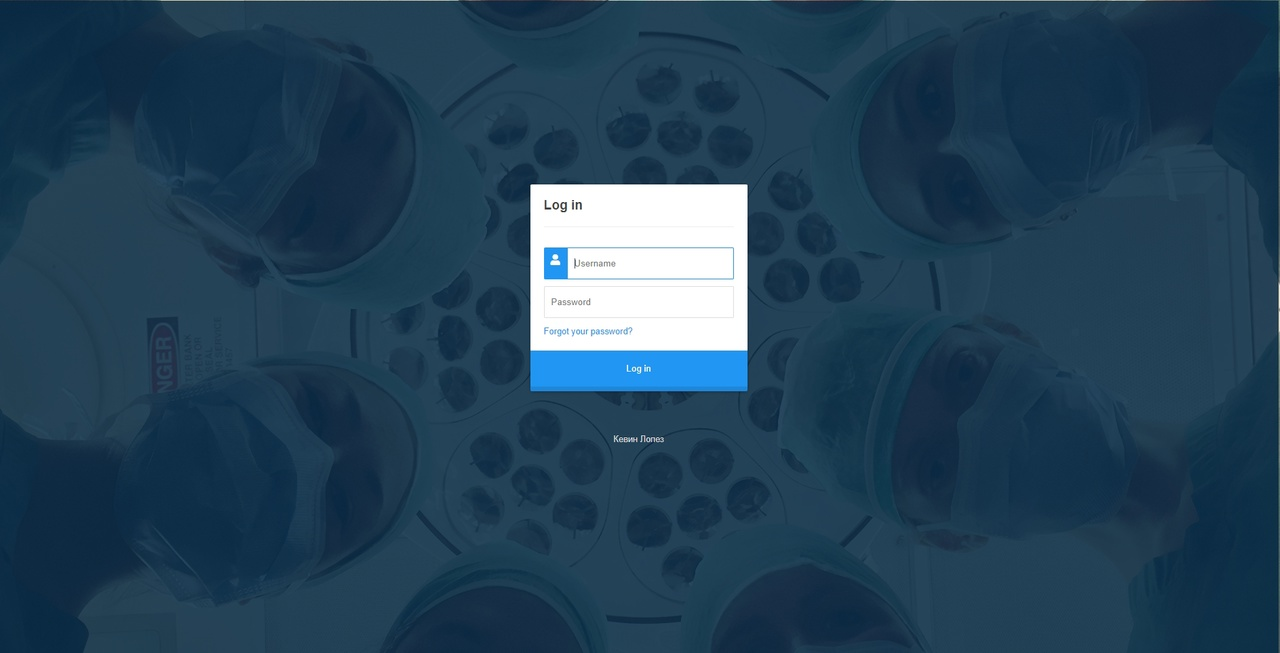
\includegraphics[width=1\linewidth]{Login}}
\caption{Главная страница сайта для ввода имени пользователя и пароля}
\label{image:log}
\end{figure}

Случай использования: пользователь или пароль не вошли в систему;
Предусловие: открыта домашняя страница;
Тестовый случай: логин или пароль врача;
Ожидаемый результат: система показывает ошибку при вводе имени пользователя или пароля.

Если имя пользователя или пароль неверны, веб-страница будет перенаправлена на окно ошибки, как показано на рисунке \ref{image:error}.

\begin{figure}
	\center{
\includegraphics[width=0.3\linewidth]{error}}
	\caption{Окно ошибки}
	\label{image:error}
\end{figure}

Сайт содержит навигационное меню с левой стороны, которое облегчает врачу поиск специальностей или регистрацию нового врача или пациента.
На рисунке \ref{image:menu} показана страница с навигационным меню.

\begin{figure}
	\center{
\includegraphics[width=0.2\linewidth]{menu}}
	\caption{Меню навигации}
	\label{image:menu}
\end{figure}

Случай использования: прием нового пациента;
Предусловие: эффективная валидация имени пользователя и пароля;
Тестовый случай: заполнение формы для регистрации нового пациента;
Ожидаемый результат: форма заполнена и эффективно зарегистрирована в базе данных.

На рисунке \ref{image:pac} показана страница с формой регистрации пациентов для приема в медицинскую лабораторию.

\begin{figure}
	\center{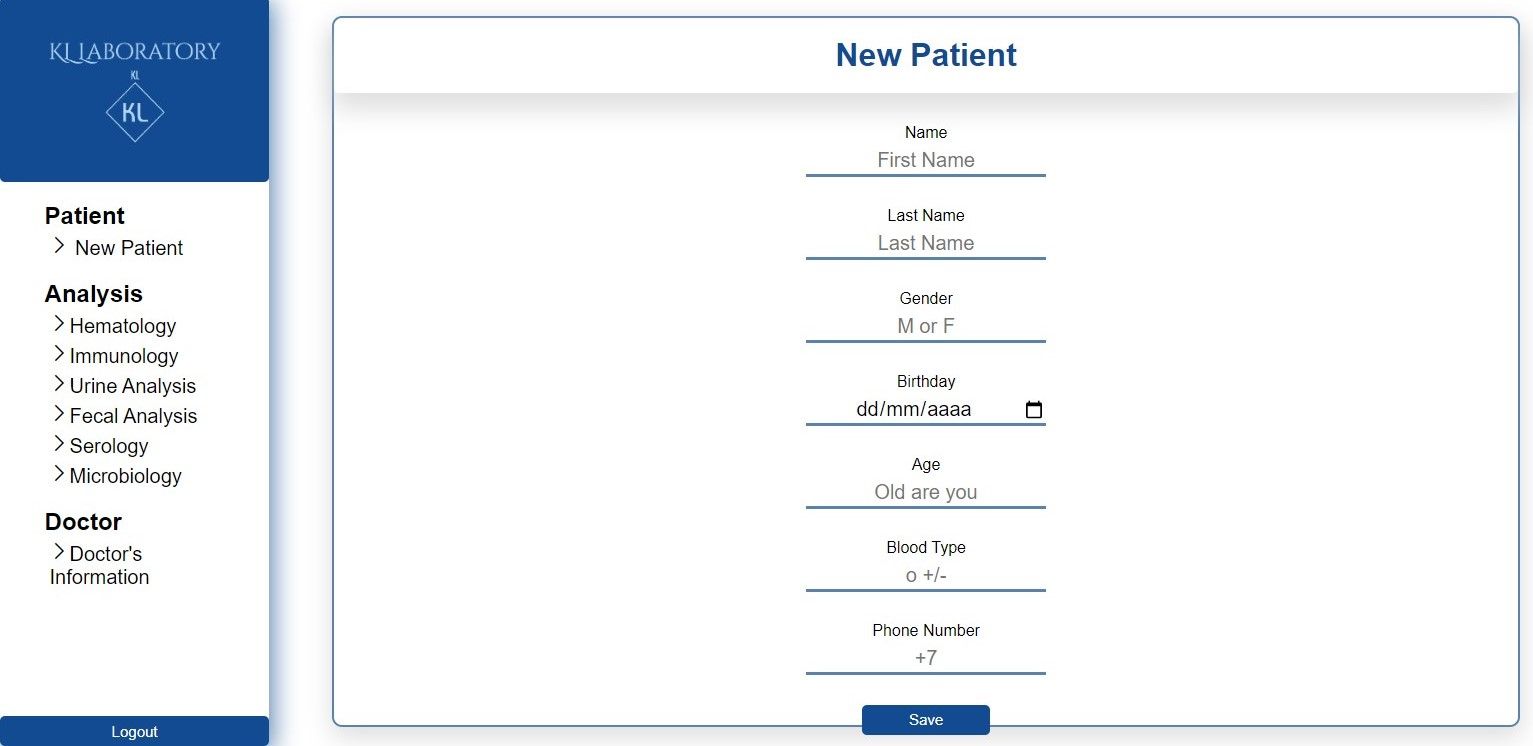
\includegraphics[width=1\linewidth]{pagi1}}
	\caption{Форма для нового пациента}
	\label{image:pac}
\end{figure}

Случай использования: вход в систему нового врача;
Предусловие: пользователь выбирает в навигационном меню регистрацию нового врача;
Тестовый случай: заполнение формы для регистрации нового врача;
Ожидаемый результат: форма заполнена и эффективно зарегистрирована в базе данных.

На рисунке \ref{image:doc} показана страница с регистрационной формой для новых врачей, поступающих в медицинскую лабораторию.

\begin{figure}
	\center{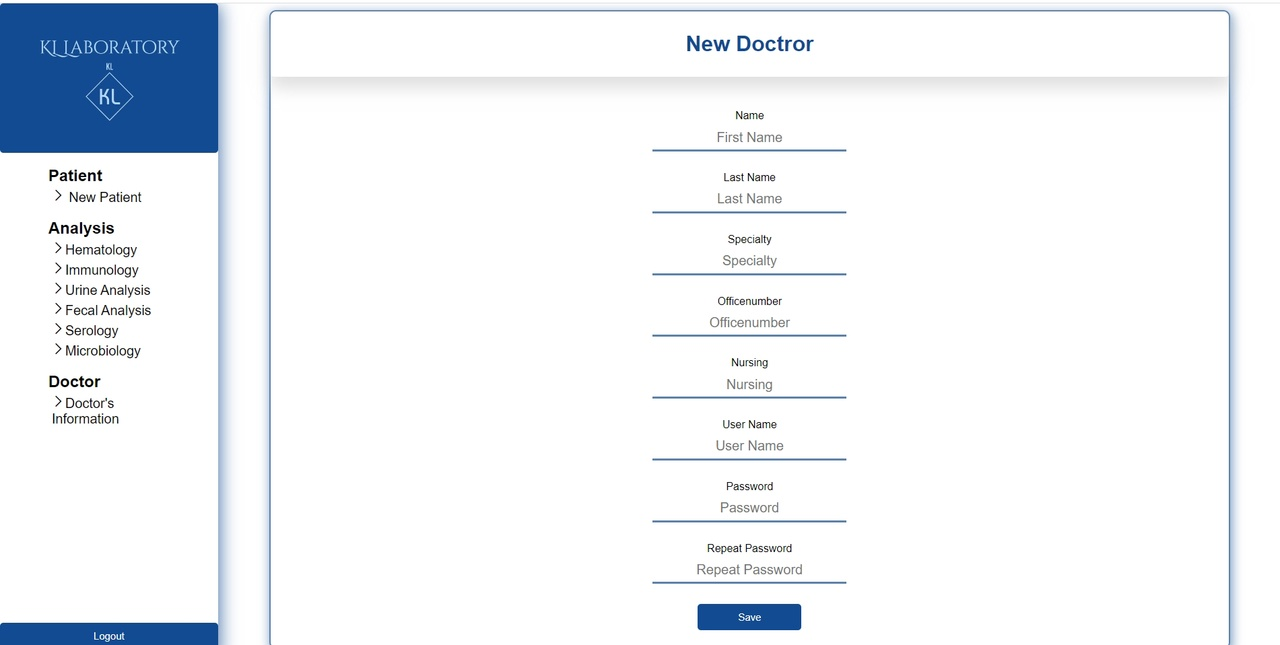
\includegraphics[width=1\linewidth]{pag3}}
	\caption{Форма нового врача}
	\label{image:doc}
\end{figure}

Случай использования: регистрация процессов и обследований пациентов;
Предусловие: пользователь выбирает в навигационном меню специальность для регистрации пациента;
Тестовый случай: заполнение формы с процедурами, результатами и лечением пациента;
Ожидаемый результат: заполненная форма и эффективная регистрация в базе данных в таблице каждой специальности.

На рисунке \ref{image:ana} показана страница с регистрационной формой для одной из специальностей медицинской лаборатории.

\begin{figure}
	\center{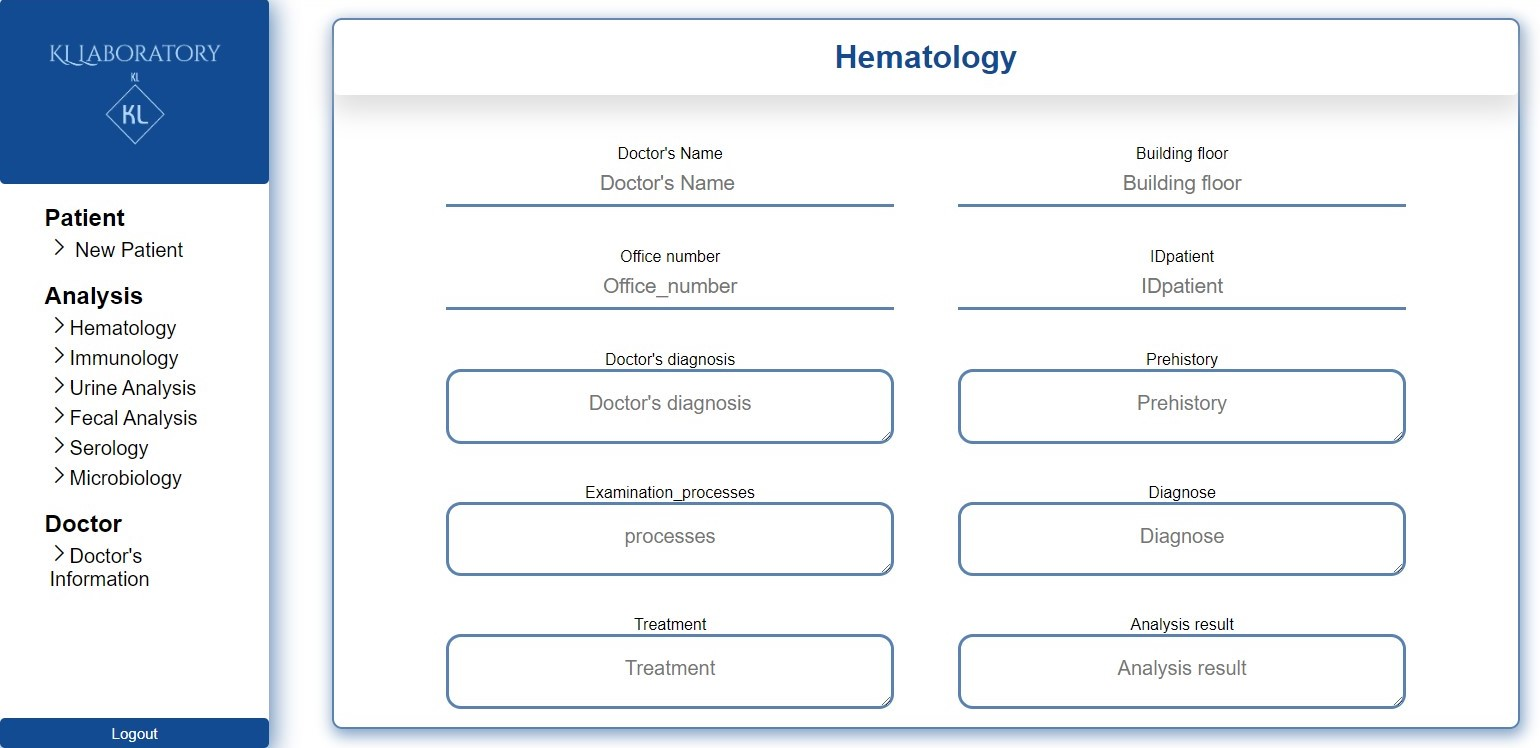
\includegraphics[width=1\linewidth]{pag2}}
	\caption{Форма специализации}
	\label{image:ana}
\end{figure}

Случай использования: верификация пациентов в системе;
Предусловие: пользователь выбирает опцию информации в навигационном меню;
Тестовый случай: визуализация таблицы с записями пациентов, внесенными в базу данных;
Ожидаемый результат: отображение таблицы со всей информацией о пациентах, внесенной в медицинскую лабораторию.

На рисунке \ref{image:infor} показана страница базы данных с информацией о пациенте.

\begin{figure}
	\center{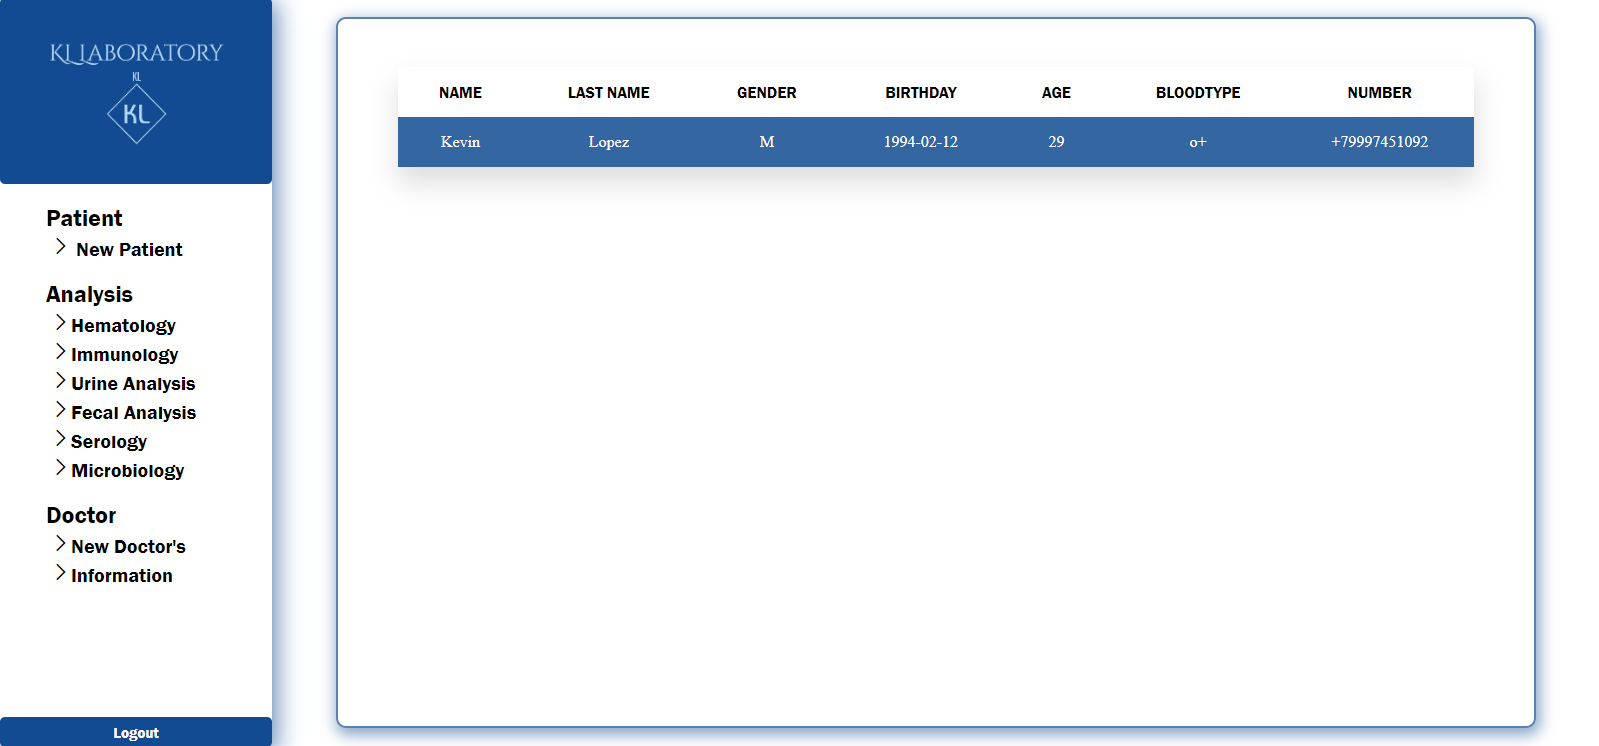
\includegraphics[width=1\linewidth]{inform}}
	\caption{Пациенты, зарегистрированные в базе данных}
	\label{image:infor}
\end{figure}

\subsection{Тестирование интерфейсов в среде веб-страницы}

Пример пользовательского тестирования, включающий запуск и навигацию по веб-странице, будет использован для объяснения процесса разработки наборов тестов для интерфейсов.

В таблице \ref{table:test} показаны различные тестовые наборы для проверки функциональности пользовательского интерфейса во время его запуска и отладки.

\begin{xltabular}{\textwidth}{|X|X|X|X|}
	\caption{Тестовые наборы для отладки интерфейса веб-сайта медицинской лаборатории.\label{table:test}}\\
	\hline \centrow Проверяемая ситуация & \centrow Действия пользователя & \centrow Входные данные & \centrow Реакция системы \\
	\hline \centrow 1 & \centrow 2 & \centrow 3 & \centrow 4\\
	\endfirsthead
	\caption*{Продолжение таблицы \ref{table:test}}\\
	\hline \centrow 1 & \centrow 2 & \centrow 3 & \centrow 4\\
	\finishhead
	\hline
	Пользователь не ввел имя пользователя или пароль в начальное поле. & Пользователь не вводил цифры, символы или буквы в поля логина и пароля врача. & Поле ввода имени пользователя и пароля пусто. & Система отображает временное сообщение
	``введите имя пользователя и пароль''.\\ \hline
	Перейти на главную страницу. & Пользователь правильно введите имя пользователя и пароль врача. & Пользователь правильно вводит данные врача, а затем нажимает кнопку для входа в систему. & Система я открываю главную страницу, которая является формой для регистрации нового пациента.\\ \hline
	Регистрация нового пациента. & Пользователь заполняет поля формы. & Врач или медсестра вводит личную информацию пациента, который собирается поступить в медицинскую лабораторию.Затем нажмите кнопку сохранить. & Система проверяет информацию, введенную в поля формы для записи в таблицу базы данных.\\ \hline
	Заполнение специальной формы. & Пользователь выбирает специальность в лаборатории. & Врач или медсестра выбирают специальность, необходимую пациенту, и записывают проводимые с ним процедуры и обследования.Затем нажмите кнопку сохранить. & Система проверяет и записывает информацию, введенную в поля формы, и сохраняет в табеле каждой специальности в базе данных.\\ \hline
	Регистрация нового врача. & Пользователь регистрирует нового врача в медицинской лаборатории. & Врач или медсестра запишут информацию о новом враче, который будет работать в медицинской лаборатории. А затем нажмите кнопку сохранения. & Система проверяет информацию и заносит в таблицу врачей в базе данных.\\ \hline
	Отображать информацию. & Пользователь хочет видеть информацию о пациентах. & В информационном поле отображается табала со всеми личными данными пациентов, зарегистрированных в медицинской лаборатории. & Система развертывает таблицу, выполняя запрос из базы данных.\\ \hline 
	Выход из системы & Пользователь желает покинуть сеанс врача. & Пользователь нажимает кнопку выхода в нижней части меню навигации. & Система завершает сеанс и возвращается на главный экран, чтобы снова ввести имя пользователя и пароль.\\ \hline	
\end{xltabular}
	\newsection
\centertocsection{ЗАКЛЮЧЕНИЕ}

В заключение следует отметить, что создание веб-сайта для медицинской лаборатории может значительно улучшить коммуникацию между пациентами и врачами, в свою очередь повышая эффективность работы лаборатории. Однако важно учитывать информационную безопасность, чтобы защитить конфиденциальность пациентов. В целом, внедрение информационных технологий в веб-сайт медицинской лаборатории может стать ценной инвестицией для повышения качества обслуживания и удовлетворенности пациентов.
Основные выводы по работе:

\begin{enumerate}
\item Проведен анализ проблемы. Выявлена потребность в медицинской лаборатории.
\item Разработана концептуальная модель сайта.
\item Разработана модель данных системы. Определены требования к системе.
\item Выполнено проектирование веб-сайта. 
\item Разработана архитектура базы данных. Реализована связь сайта с базой данных. 
\item Разработан пользовательский интерфейс сайта.
\item Веб-сайт был внедрен и протестирован. Проведено тестирование системы.
\end{enumerate}

Были выполнены все требования, изложенные в техническом задании, и решены все задачи, поставленные в начале проекта разработки. В результате был получен адаптированный дизайн сайта для медицинской лаборатории.
	\newsection
\centertocsection{СПИСОК ИСПОЛЬЗОВАННЫХ ИСТОЧНИКОВ}

\begin{hyphenrules}{nohyphenation} %отключение переноса слов в содержании
  \begin{thebibliography}{9}

    \bibitem{hHTLM} Mclibre.org: сайт. – URL: https://www.mclibre.org/consultar/htmlcss/otros/historia-resumen.html (дата обращения: 23.05.2023).
    \bibitem{website} UPanama: Universidad de Panama: офиц. сайт. – URL: https://upanama.educativa.org/(дата обращения: 23.05.2023).
    \bibitem{web} BOE.es: офиц. сайт. – URL:\\    https://www.boe.es/eli/es/rd/2022/04/05/243/con (дата обращения: 24.05.2023).
    \bibitem{php} Caracteristicasdel.com: сайт. – URL: \\https://www.caracteristicasdel.com/tecnologia/caracteristicasdelphp.html (дата обращения: 24.05.2023).
    \bibitem{php1} Rockcontent: офиц. сайт. – URL: https://rockcontent.com/es/blog/php/ (дата обращения: 24.05.2023).
    \bibitem{css} HubSpot: офиц. сайт. – URL: https://blog.hubspot.es/website/que-es-css (дата обращения: 25.05.2023).
    \bibitem{css1} Lenguajecss: офиц. сайт. – URL: https://lenguajecss.com/css/introduccion/que-es-css/ 
    (дата обращения: 25.05.2023).
    \bibitem{php2} DOF: офиц. сайт. – URL: \\https://dof.gob.mx/nota detalle.php?codigo=5496728fecha=08/09/2017gsc.tab=0 
    (дата обращения: 26.05.2023).
    \bibitem{html1} MDN: webdocs: офиц. сайт. – URL: \\https://developer.mozilla.org/es/docs/Web/HTML (дата обращения: 26.05.2023).
    \bibitem{html2} HostGator: офиц. сайт. – URL: https://www.hostgator.mx/blog/pagina-web-en-html/ (дата обращения: 26.05.2023).
    \bibitem{php3} IONOS: офиц. сайт. – URL: https://www.ionos.es/digitalguide/paginas-web/creacion-de-paginas-web (дата обращения: 26.05.2023).
   	\bibitem{php4} MCLIBRE: сайт. – URL: https://www.mclibre.org/consultar/php/lecciones/php-primeras-paginas.html (дата обращения: 27.05.2023).
    \bibitem{css2} ЭVORAGINE: офиц. сайт. – URL: https://voragine.net/weblogs/ (дата обращения: 27.05.2023).
    \bibitem{css3} RIBOSOMATIC: офиц. сайт. – URL: \\https://www.ribosomatic.com/articulos/ (дата обращения: 28.05.2023).
    \bibitem{css4} WEBSITERATING: офиц. сайт. – URL: \\https://www.websiterating.com/es/resources/html-css-php-cheat-sheet/ (дата обращения: 28.05.2023).
    \bibitem{CSP} DISENOWEBAKUS: офиц. сайт. – URL: \\https://disenowebakus.net/un-paso-mas-alla-de-html-y-css.php (дата обращения: 28.05.2023).
    \bibitem{CSP1} DOMESTIKA: сайт. – URL: https://www.domestika.org/es/forums/5-programacion-cliente/topics/ (дата обращения: 28.05.2023).
    \bibitem{CSP2} KINSTA: офиц. сайт. – URL: https://kinsta.com/es/base-de-conocimiento/editar-codigo-wordpress/ (дата обращения: 29.05.2023).
    \bibitem{PSS} SALESFORCE: офиц. сайт. – URL: \\https://help.salesforce.com/s/articleView?id=sf.mc\_es\_php\_conv\_samples.htm\&type=5 (дата обращения: 29.05.2023).
    \bibitem{HTMLL} VADAVO: сайт. – URL: https://www.vadavo.com/blog/html-que-es-y-para-que-sirve/ (дата обращения: 29.05.2023).
    \bibitem{HTML3} CIUDADANO: сайт. – URL: https://www.ciudadano2cero.com/como-crear-una-pagina-web-en-html/ (дата обращения: 30.05.2023).
    \bibitem{HTML4} IEBS: офиц. сайт. – URL: https://www.iebschool.com/blog/que-es-etiqueta-html-analitica-usabilidad/ (дата обращения: 05.06.2023).
    \bibitem{CARACT} Nextu: офиц. сайт. – URL: https://www.nextu.com/blog/que-es-html-rc22/ (дата обращения: 30.05.2023).
    \bibitem{ondo} Ondho: сайт. – URL: \\https://ondho.com/diccionario-de-marketing/term/html/ (дата обращения: 30.05.2023).
    \bibitem{apr} Apr: офиц. сайт. – URL: https://www.aprenderaprogramar.com/index.php (дата обращения: 30.05.2023).
    \bibitem{fun} Funnel: сайт. – URL: https://funnel.mx/usar-cms-mejor-una-pagina-web-html/ (дата обращения: 31.05.2023).
    \bibitem{tokio} Tokiers: офиц. сайт. – URL: https://www.tokioschool.com/noticias/ (дата обращения: 31.05.2023).
    \bibitem{tut} Tutsplus: офиц. сайт. – URL: https://code.tutsplus.com/es/tutorials/how-to-use-php-in-html-code--cms-34378 (дата обращения: 01.06.2023).
    \bibitem{aks} Akus.net: офиц. сайт. – URL: https://disenowebakus.net/mezclando-php-y-html.php (дата обращения: 01.06.2023).
    \bibitem{dz} DzTechs: сайт. – URL: https://www.dz-techs.com/es/build-simple-php-website (дата обращения: 01.06.2023).
    \bibitem{ine} Inesem: сайт. – URL: https://www.inesem.es/revistadigital/informatica-y-tics/etiquetas-html-en-php/ (дата обращения: 02.06.2023).
    \bibitem{nor} Norfipc.com: офиц. сайт. – URL: \\https://norfipc.com/codigos/html-facil-codigo-elementos-basicos-funcionamiento.php (дата обращения: 02.06.2023).
    \bibitem{nor1} Norfipc.com: офиц. сайт. – URL: https://norfipc.com/codigos/configurar-paginas-con-css-para-imprimir-guardar-pdf.php (дата обращения: 03.06.2023).
    \bibitem{nor2} Norfipc.com: офиц. сайт. – URL: https://norfipc.com/web/como-corregir-errores-css-navegadores-web.php (дата обращения: 05.06.2023).
    \bibitem{test} WebDocs: офиц. сайт. – URL: https://developer.mozilla.org/es/docs/Learn/HTML/Introduction\_to\_HTML/Test\_your\_skills:\_HTML\_text\_basics (дата обращения: 05.06.2023).
    \bibitem{testhmt} LWP: офиц. сайт. – URL: https://www.lawebdelprogramador.com/foros/HTML/691447-Hacer-un-test.html (дата обращения: 05.06.2023).
    \bibitem{testphp} RicardoDogeek: офиц. сайт. – URL: https://ricardogeek.com/como-realizar-pruebas-unitarias-con-phpunit/ (дата обращения: 06.06.2023).
    \bibitem{test1} CosasdeDevs: сайт. – URL: https://cosasdedevs.com/posts/testar-aplicaciones-php-phpunit/ (дата обращения: 06.06.2023).
    \bibitem{test2} Codigo Naranja: сайт. – URL: https://codigonaranja.com/unit-test-php (дата обращения: 07.06.2023).
    \bibitem{test3} AULA CM: офиц. сайт. – URL: https://aulacm.com/codigos-web-css-y-html-wordpress/ (дата обращения: 07.06.2023).
    \bibitem{phpte} sukachOFF: офиц. сайт. – URL: https://sukachoff.ru/es/programmy/kommentarii-v-html-css-php-kak-zakommentirovat-na-vremya-kod-html-css-ili-php-js-kak/ (дата обращения: 07.06.2023).
    \bibitem{formula} wikiHow: офиц. сайт. – URL: \\https://es.wikihow.com/crear-formularios-HTML (дата обращения: 07.06.2023).
    \bibitem{formula1} Pamolares: офиц. сайт. – URL: https://kikopalomares.com/clases/que-son-y-como-crear-formularios-en-html (дата обращения: 07.06.2023).
    \bibitem{formula2} Manual Web: офиц. сайт. – URL: \\https://www.manualweb.net/html/formularios-html/ (дата обращения: 07.06.2023).
    \bibitem{estilo} Norfipc: офиц. сайт. – URL: https://norfipc.com/web/usar-estilos-css.html (дата обращения: 08.06.2023).
    \bibitem{estilo1} WORKANA: сайт. – URL: https://i.workana.com/glosario/css/ (дата обращения: 08.06.2023).
    \bibitem{botones} CevagrafBlog: офиц. сайт. – URL: \\https://www.cevagraf.coop/blog/como-crear-un-boton-basico-en-html-y-css/ (дата обращения: 08.06.2023).
    \bibitem{botones1} Shopify: офиц. сайт. – URL: https://www.shopify.com/es/blog/crea-un-boton-de-llamada-a-la-accion-clicable-para-tu-tema-de-shopify (дата обращения: 08.06.2023).
    \bibitem{bd} W3big: сайт. – URL: https://www.w3big.com/es/php/php-mysql-connect.html\#gsc.tab=0 (дата обращения: 08.06.2023).
    \bibitem{bd1} Programacion Facil: офиц. сайт. – URL: \\https://programacionfacil.org/blog/instalacion-de-un-servidor-para-php-y-mysql/ (дата обращения: 08.06.2023).
  \end{thebibliography}
\end{hyphenrules}

	\newsection
\section*{ПРИЛОЖЕНИЕ А \\ Представление графического материала}
\addcontentsline{toc}{section}{ПРИЛОЖЕНИЕ А Представление графического материала}

Графический материал, выполненный на отдельных листах, изображен на рисунках A.1-A.12
%\begin{itemize}
	%\item А.1 - Сведения о ВКРБ.
	%\item A.2 - Цель и задачи разработки.
	%\item A.3 - Концептуальная модель сайта.
	%\item A.4 - Диаграмма прецедентов.
	%\item A.5 - Схема базы данных.
	%\item A.6 - Диаграмма развертывания.
	%\item A.7 - Диаграмма классов.
	%\item A.8 - Дизайн интерфейса. Веб-страница авторизации.
	%\item A.9 - Дизайн интерфейса. Веб-страница регистрации пациента.
	%\item A.10 - Дизайн интерфейса. Веб-страница регистрации врача.
	%\item A.11 - Дизайн интерфейса. Веб-страница для ввода результатов анализа крови.
	%\item А.12 - Заключение.
%\end{itemize} 

\renewcommand{\thefigure}{А.\arabic{figure}} % шаблон номера рисунков


\begin{figure}
  \begin{adjustbox}{addcode={\begin{minipage}{\width}}{\caption{%
          Сведения о ВКРБ
      }\end{minipage}},rotate=90,center}
    
\includegraphics[width=1.3\linewidth]{плакат1.png}
  \end{adjustbox}
  \label{pl1:image}      
\end{figure}

\begin{figure}
  \begin{adjustbox}{addcode={\begin{minipage}{\width}}{\caption{%
          Цель и задачи работы
      }\end{minipage}},rotate=90,center}
    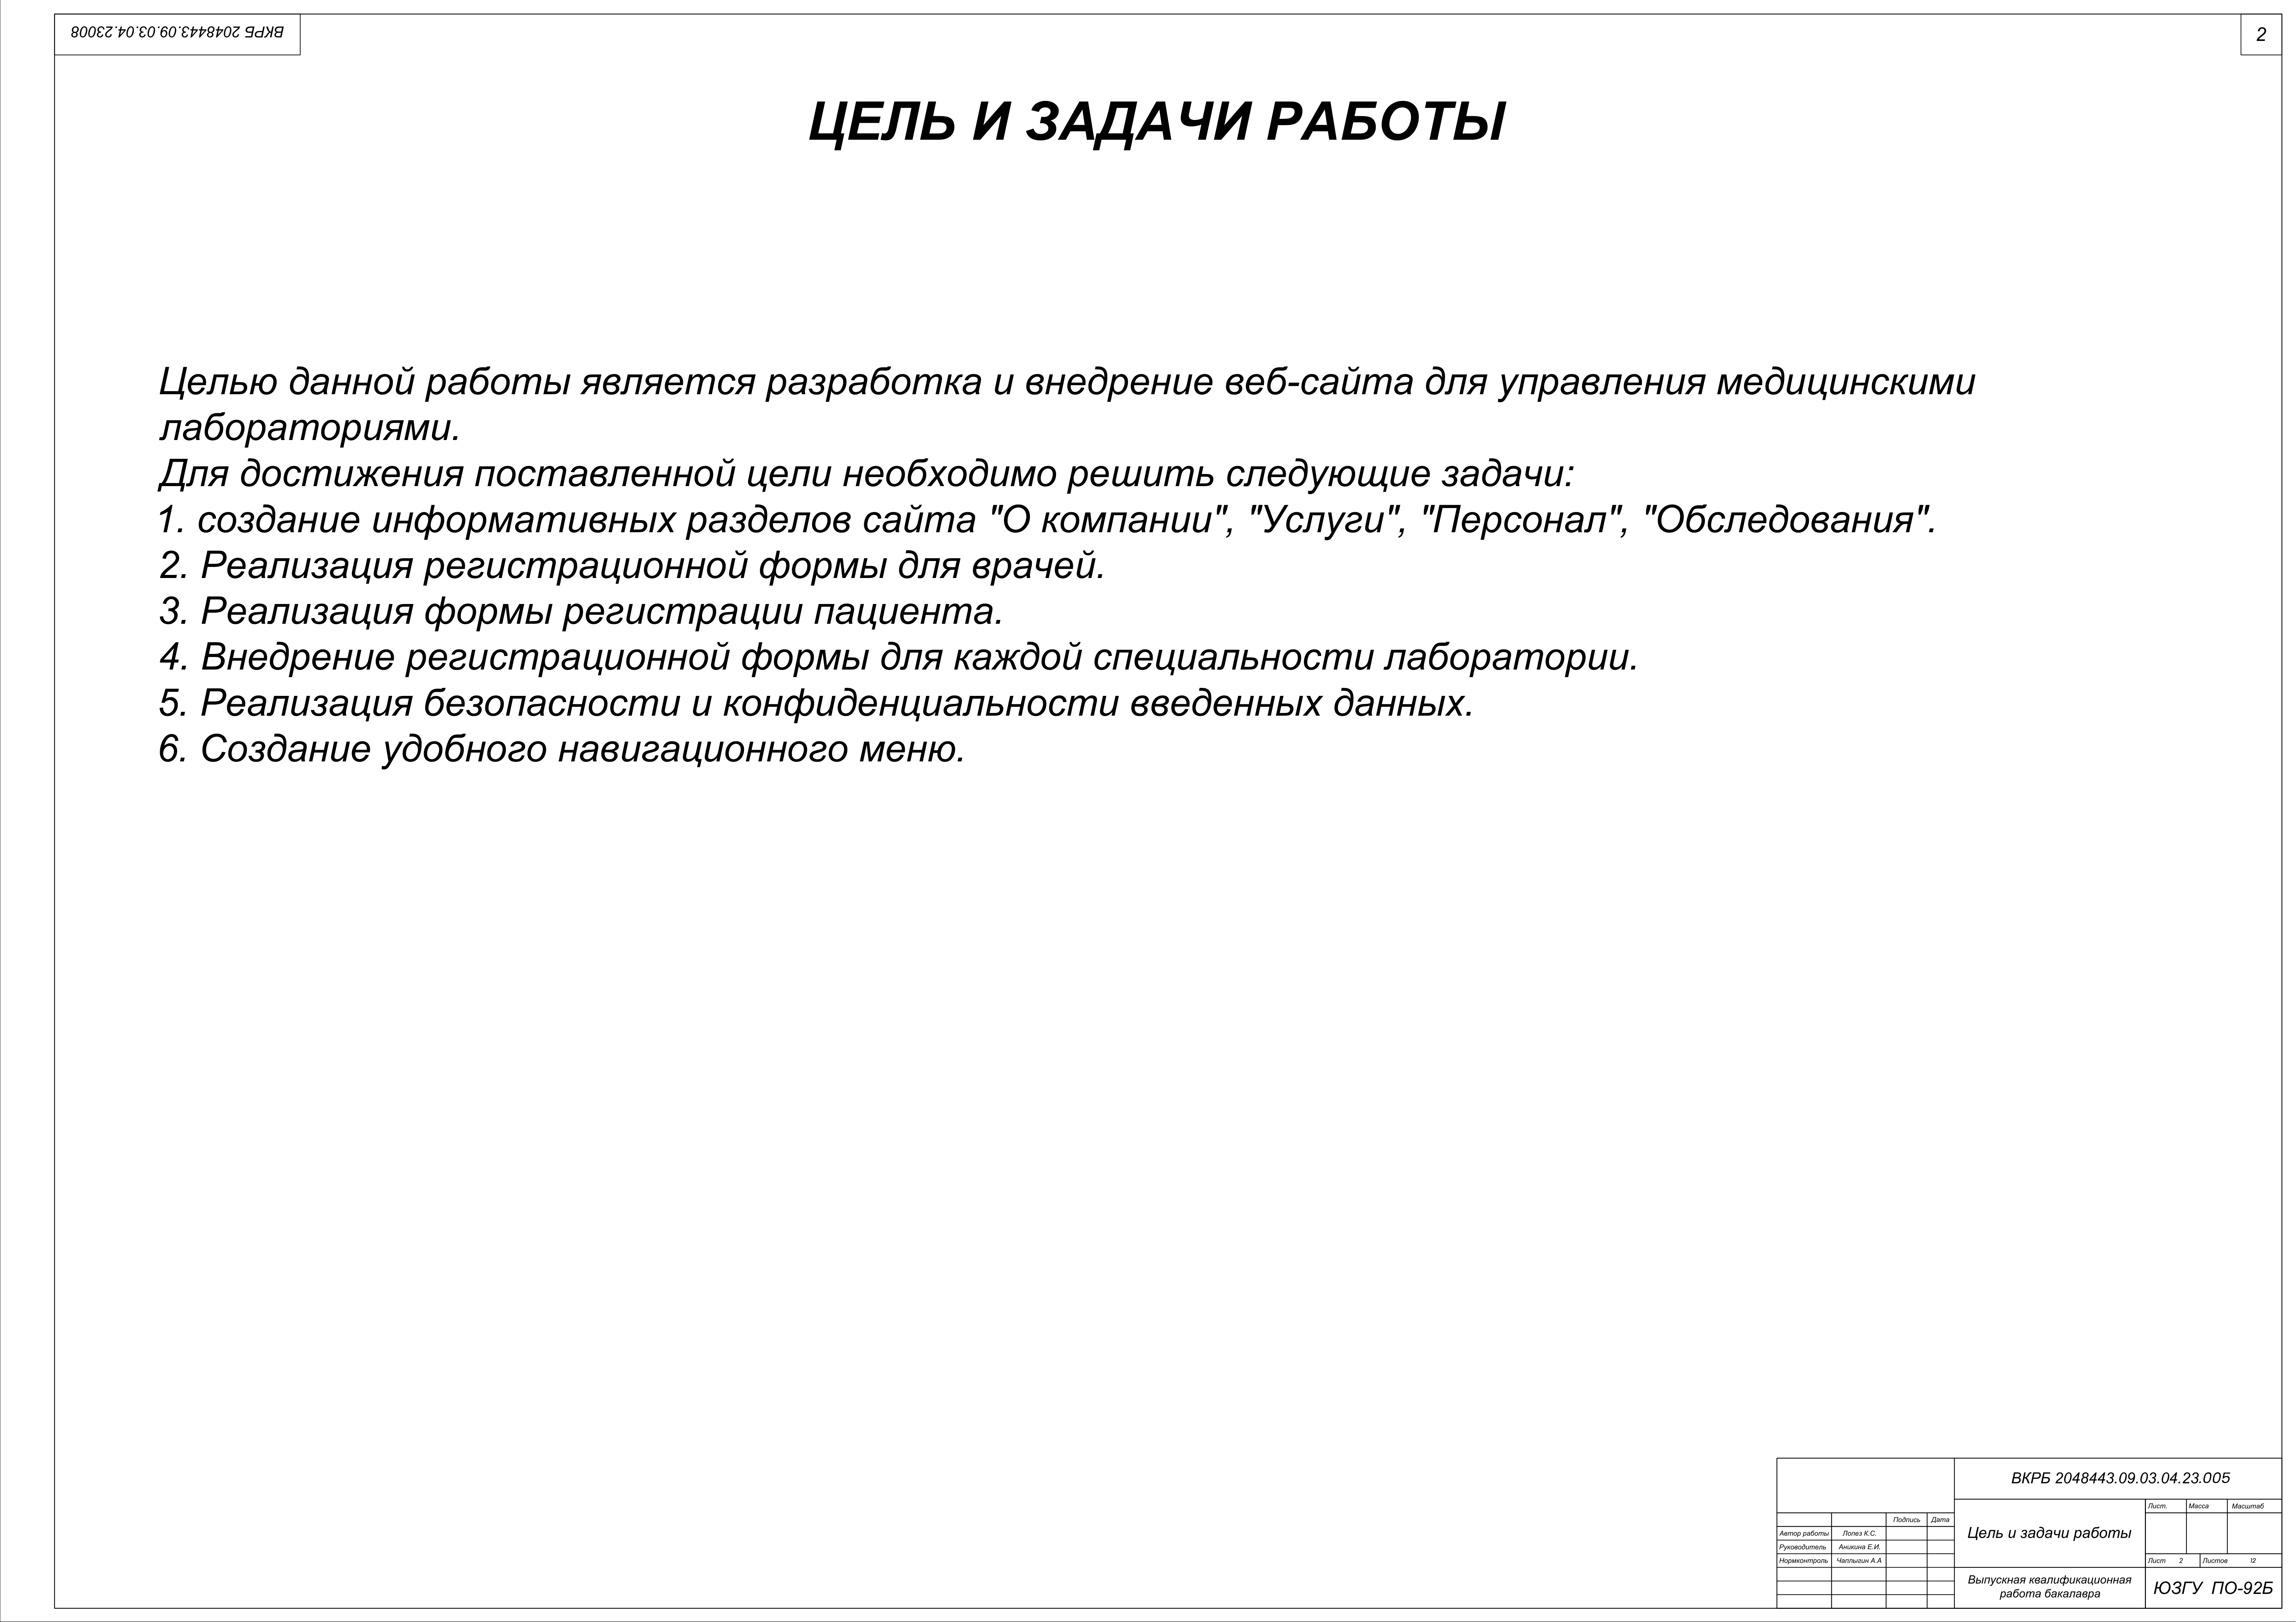
\includegraphics[width=1.3\linewidth]{плакат2.png}
  \end{adjustbox}
  \label{pl2:image}      
\end{figure}

\begin{figure}
  \begin{adjustbox}{addcode={\begin{minipage}{\width}}{\caption{%
          Концептуальная модель сайта
      }\end{minipage}},rotate=90,center}
    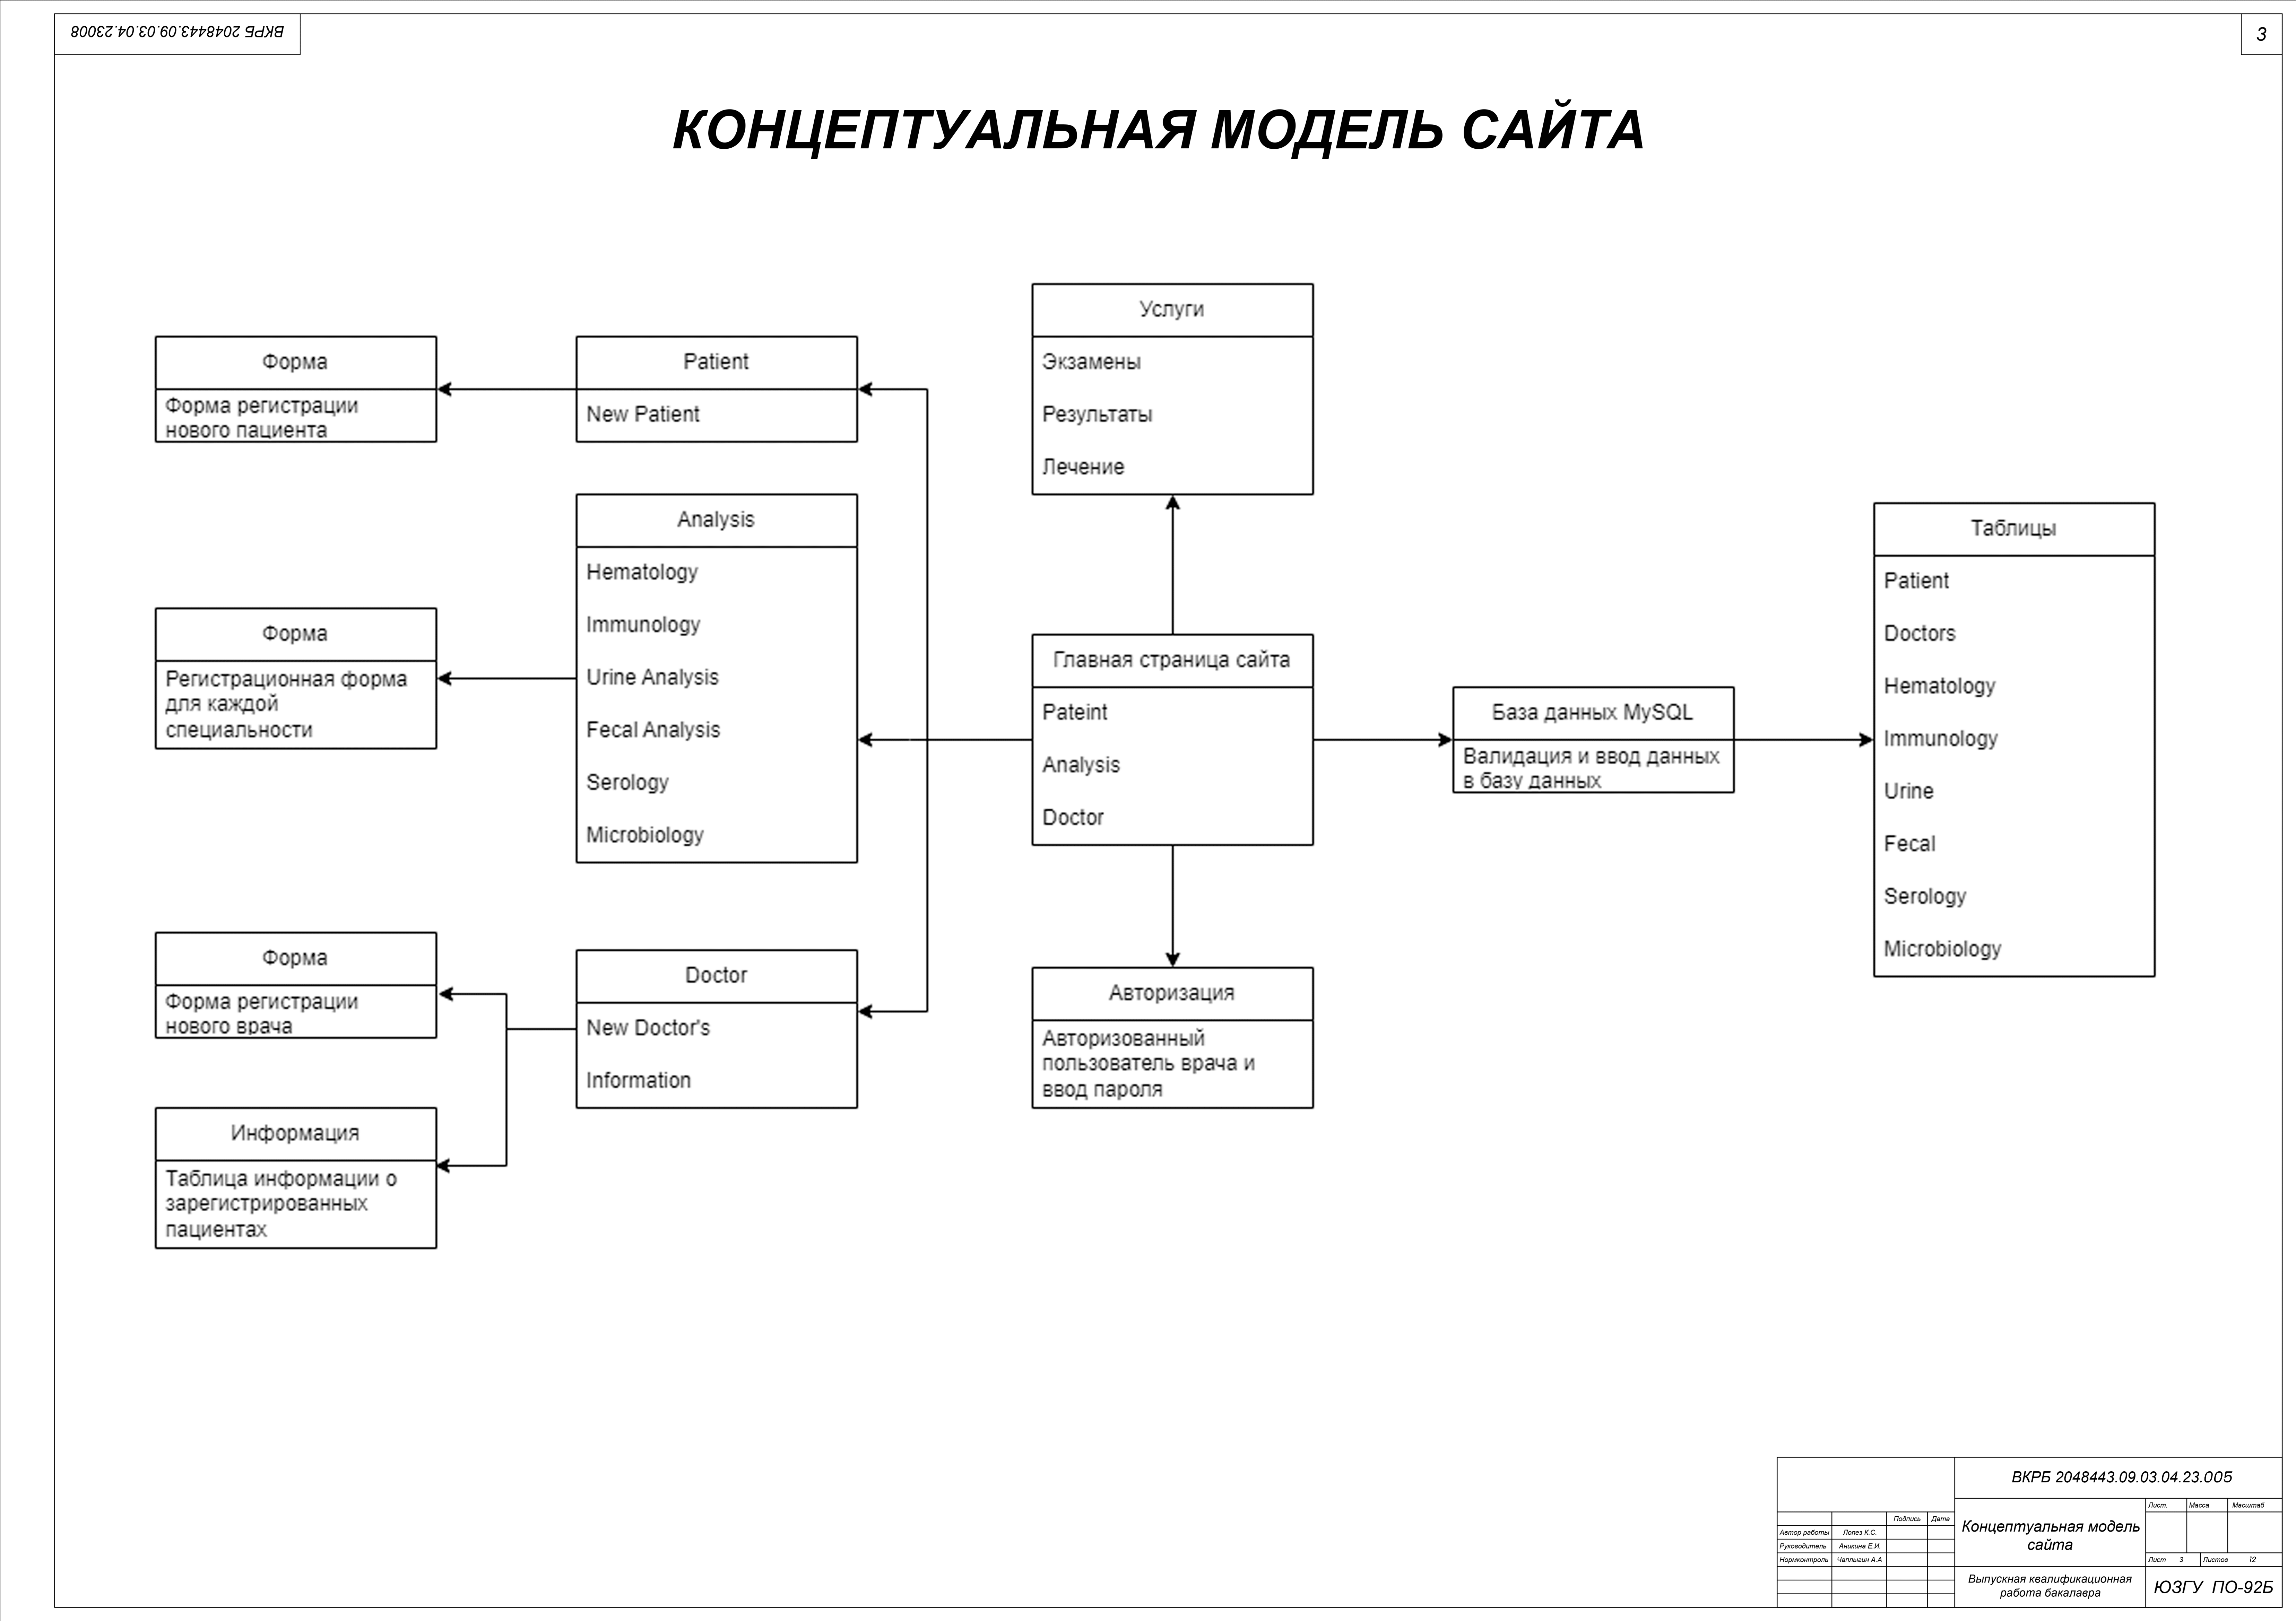
\includegraphics[width=1.3\linewidth]{плакат3.png}
  \end{adjustbox}
  \label{pl3:image}      
\end{figure}

\begin{figure}
	\begin{adjustbox}{addcode={\begin{minipage}{\width}}{\caption{%
						Диаграмма прецедентов
			}\end{minipage}},rotate=90,center}
		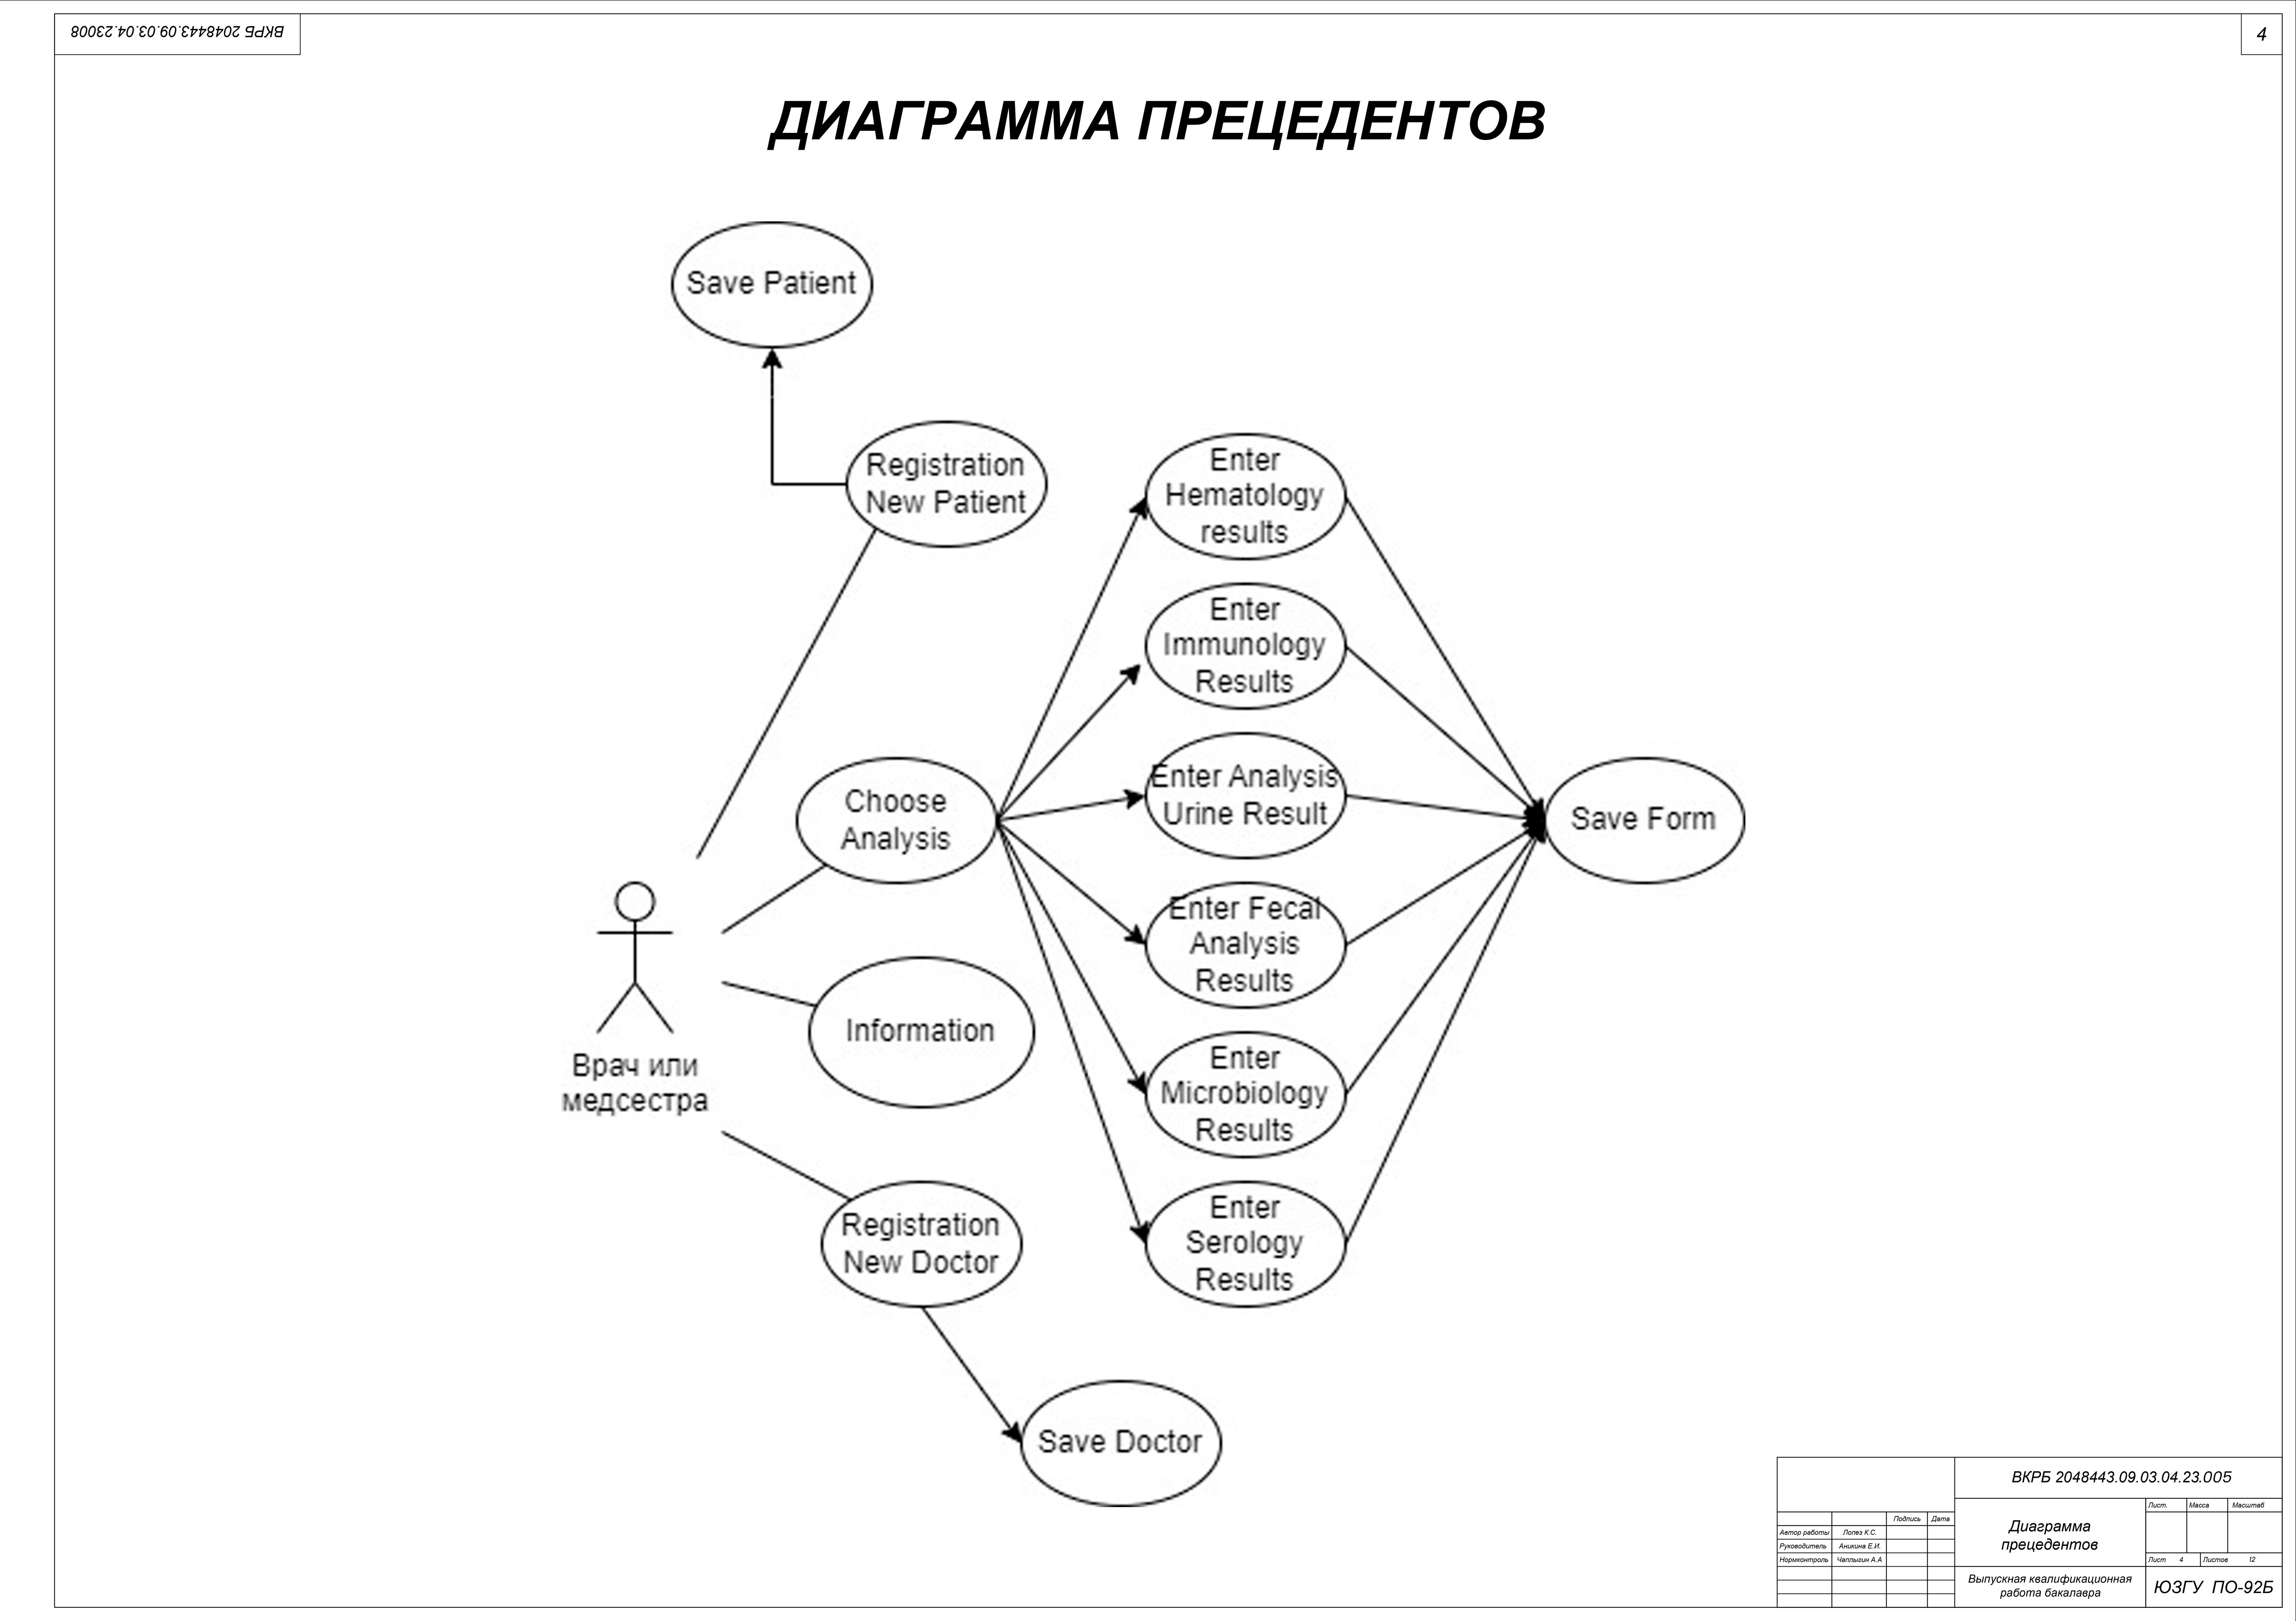
\includegraphics[width=1.3\linewidth]{плакат4.png}
	\end{adjustbox}
	\label{pl4:image}      
\end{figure}

\begin{figure}
	\begin{adjustbox}{addcode={\begin{minipage}{\width}}{\caption{%
						Схема базы данных
			}\end{minipage}},rotate=90,center}
		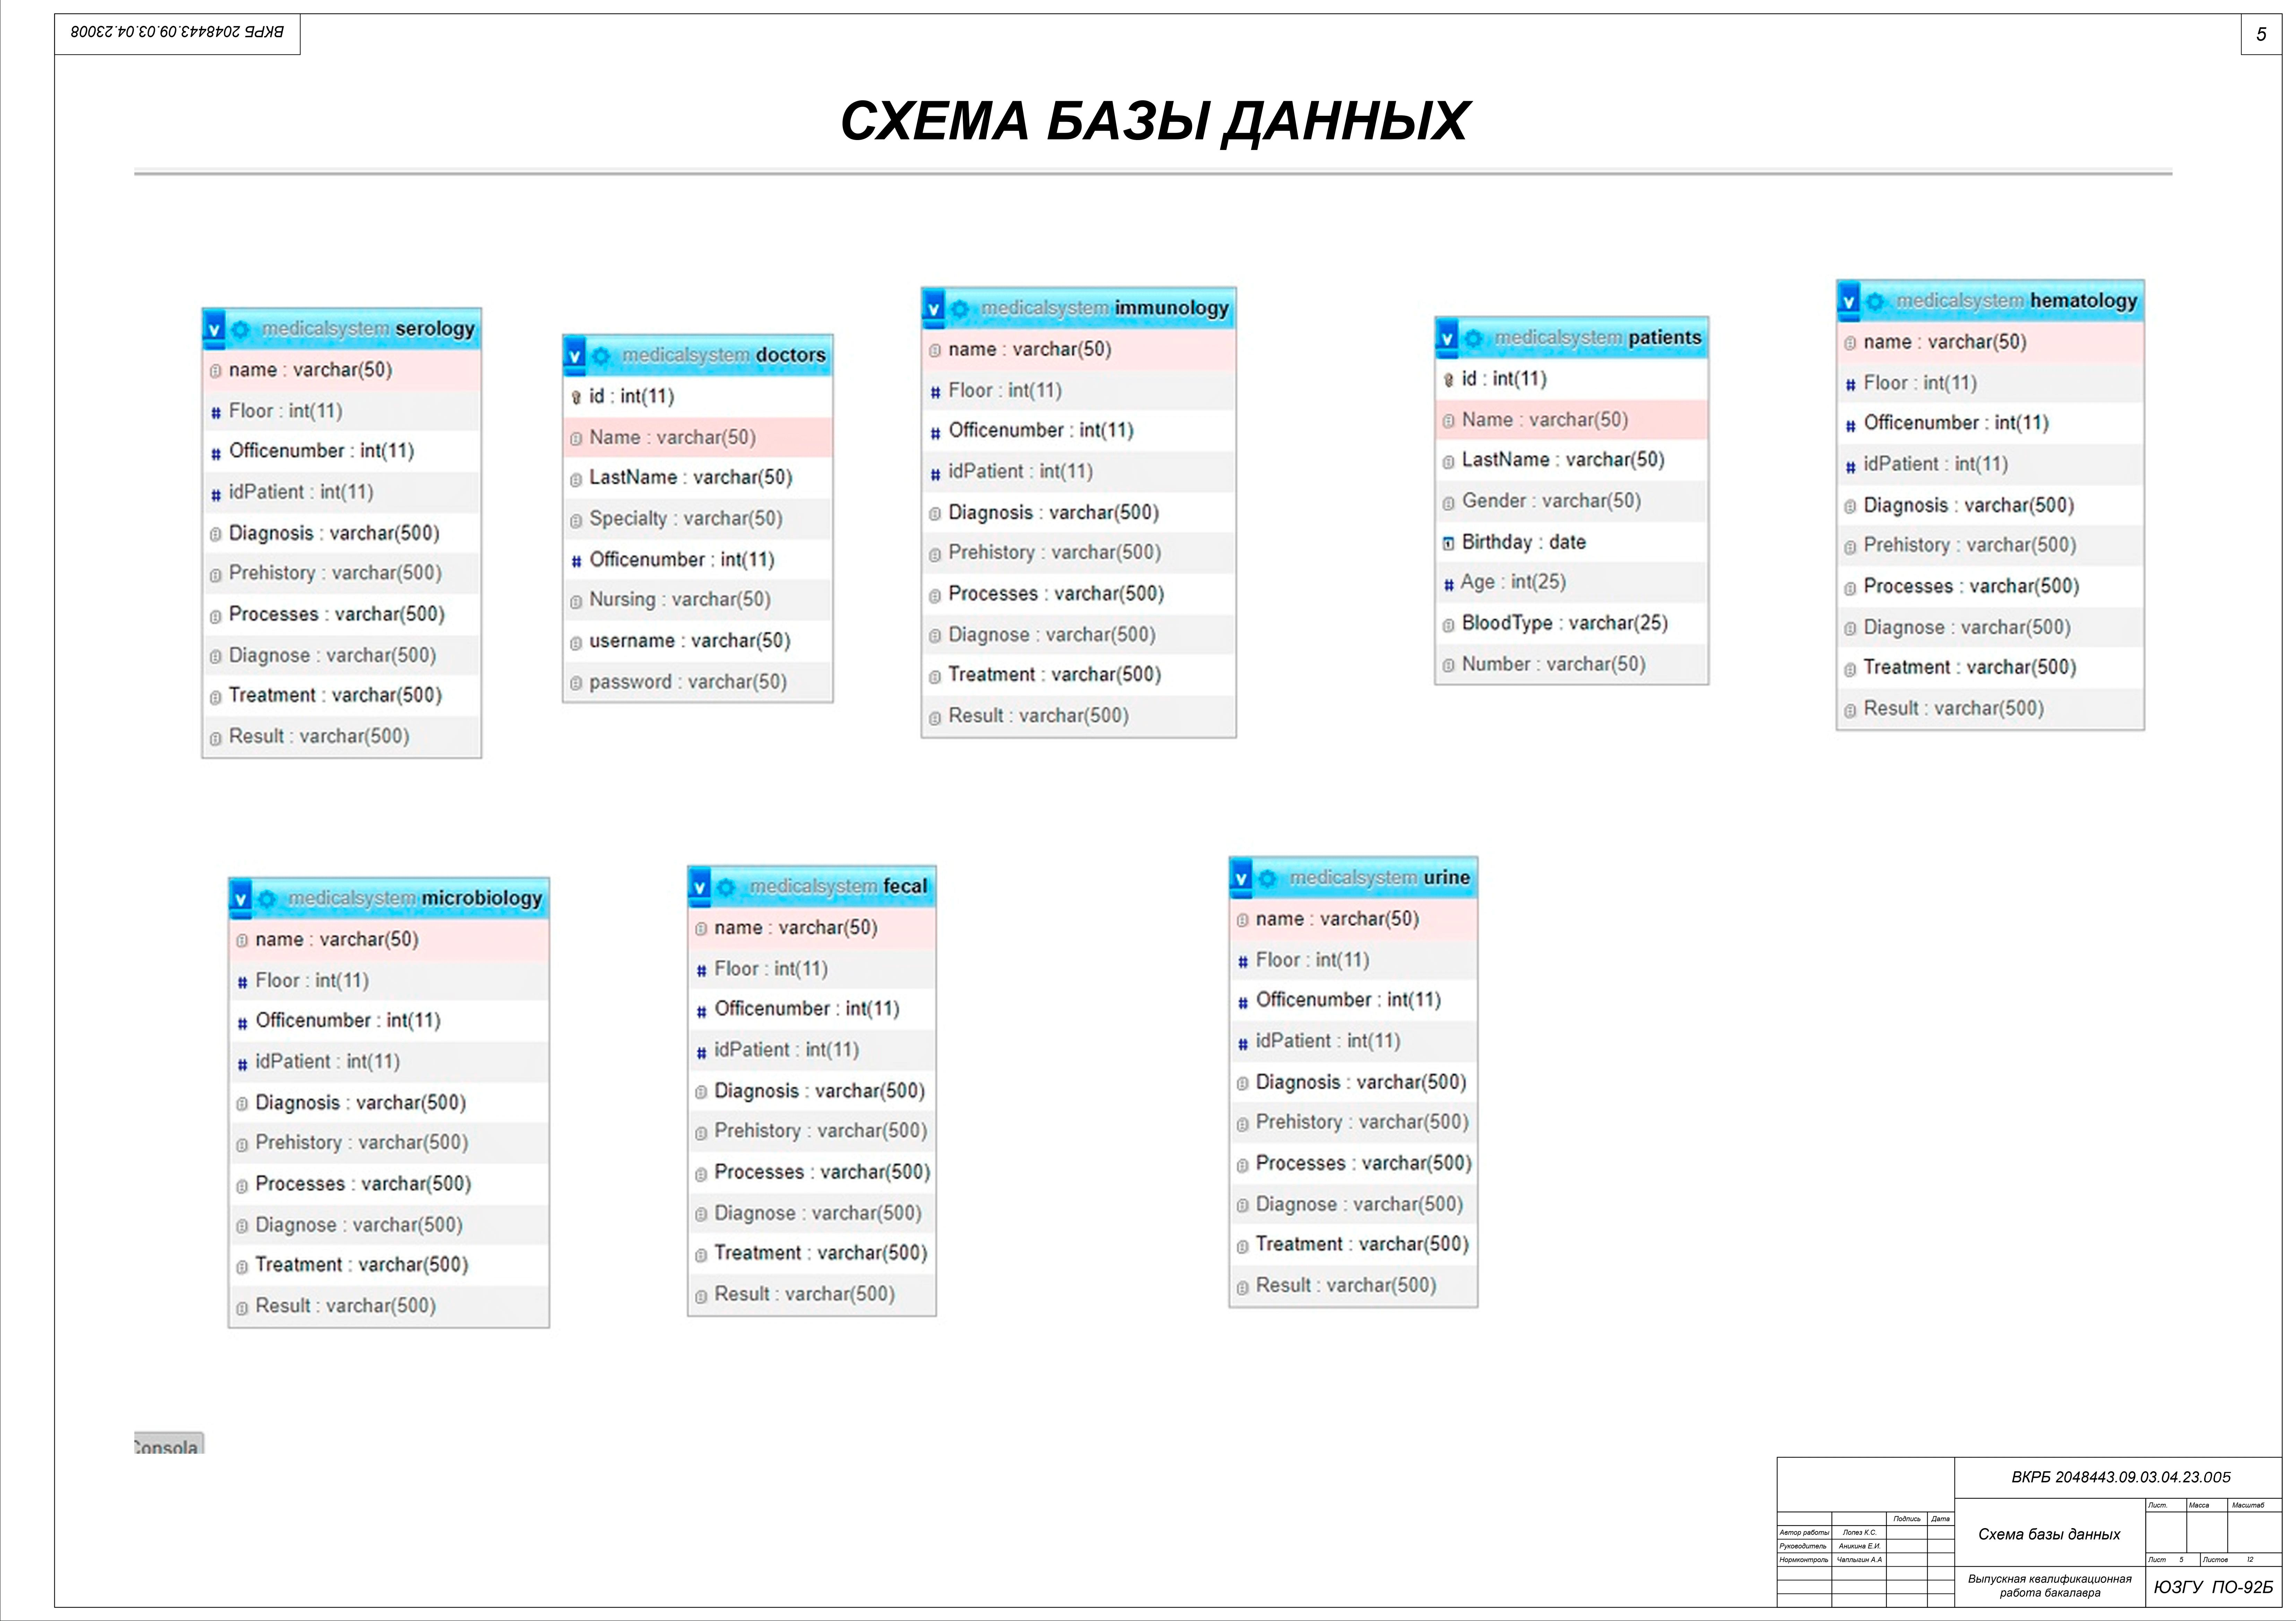
\includegraphics[width=1.3\linewidth]{плакат5.png}
	\end{adjustbox}
	\label{pl5:image}      
\end{figure}

\begin{figure}
	\begin{adjustbox}{addcode={\begin{minipage}{\width}}{\caption{%
						Диаграмма развертывания
			}\end{minipage}},rotate=90,center}
		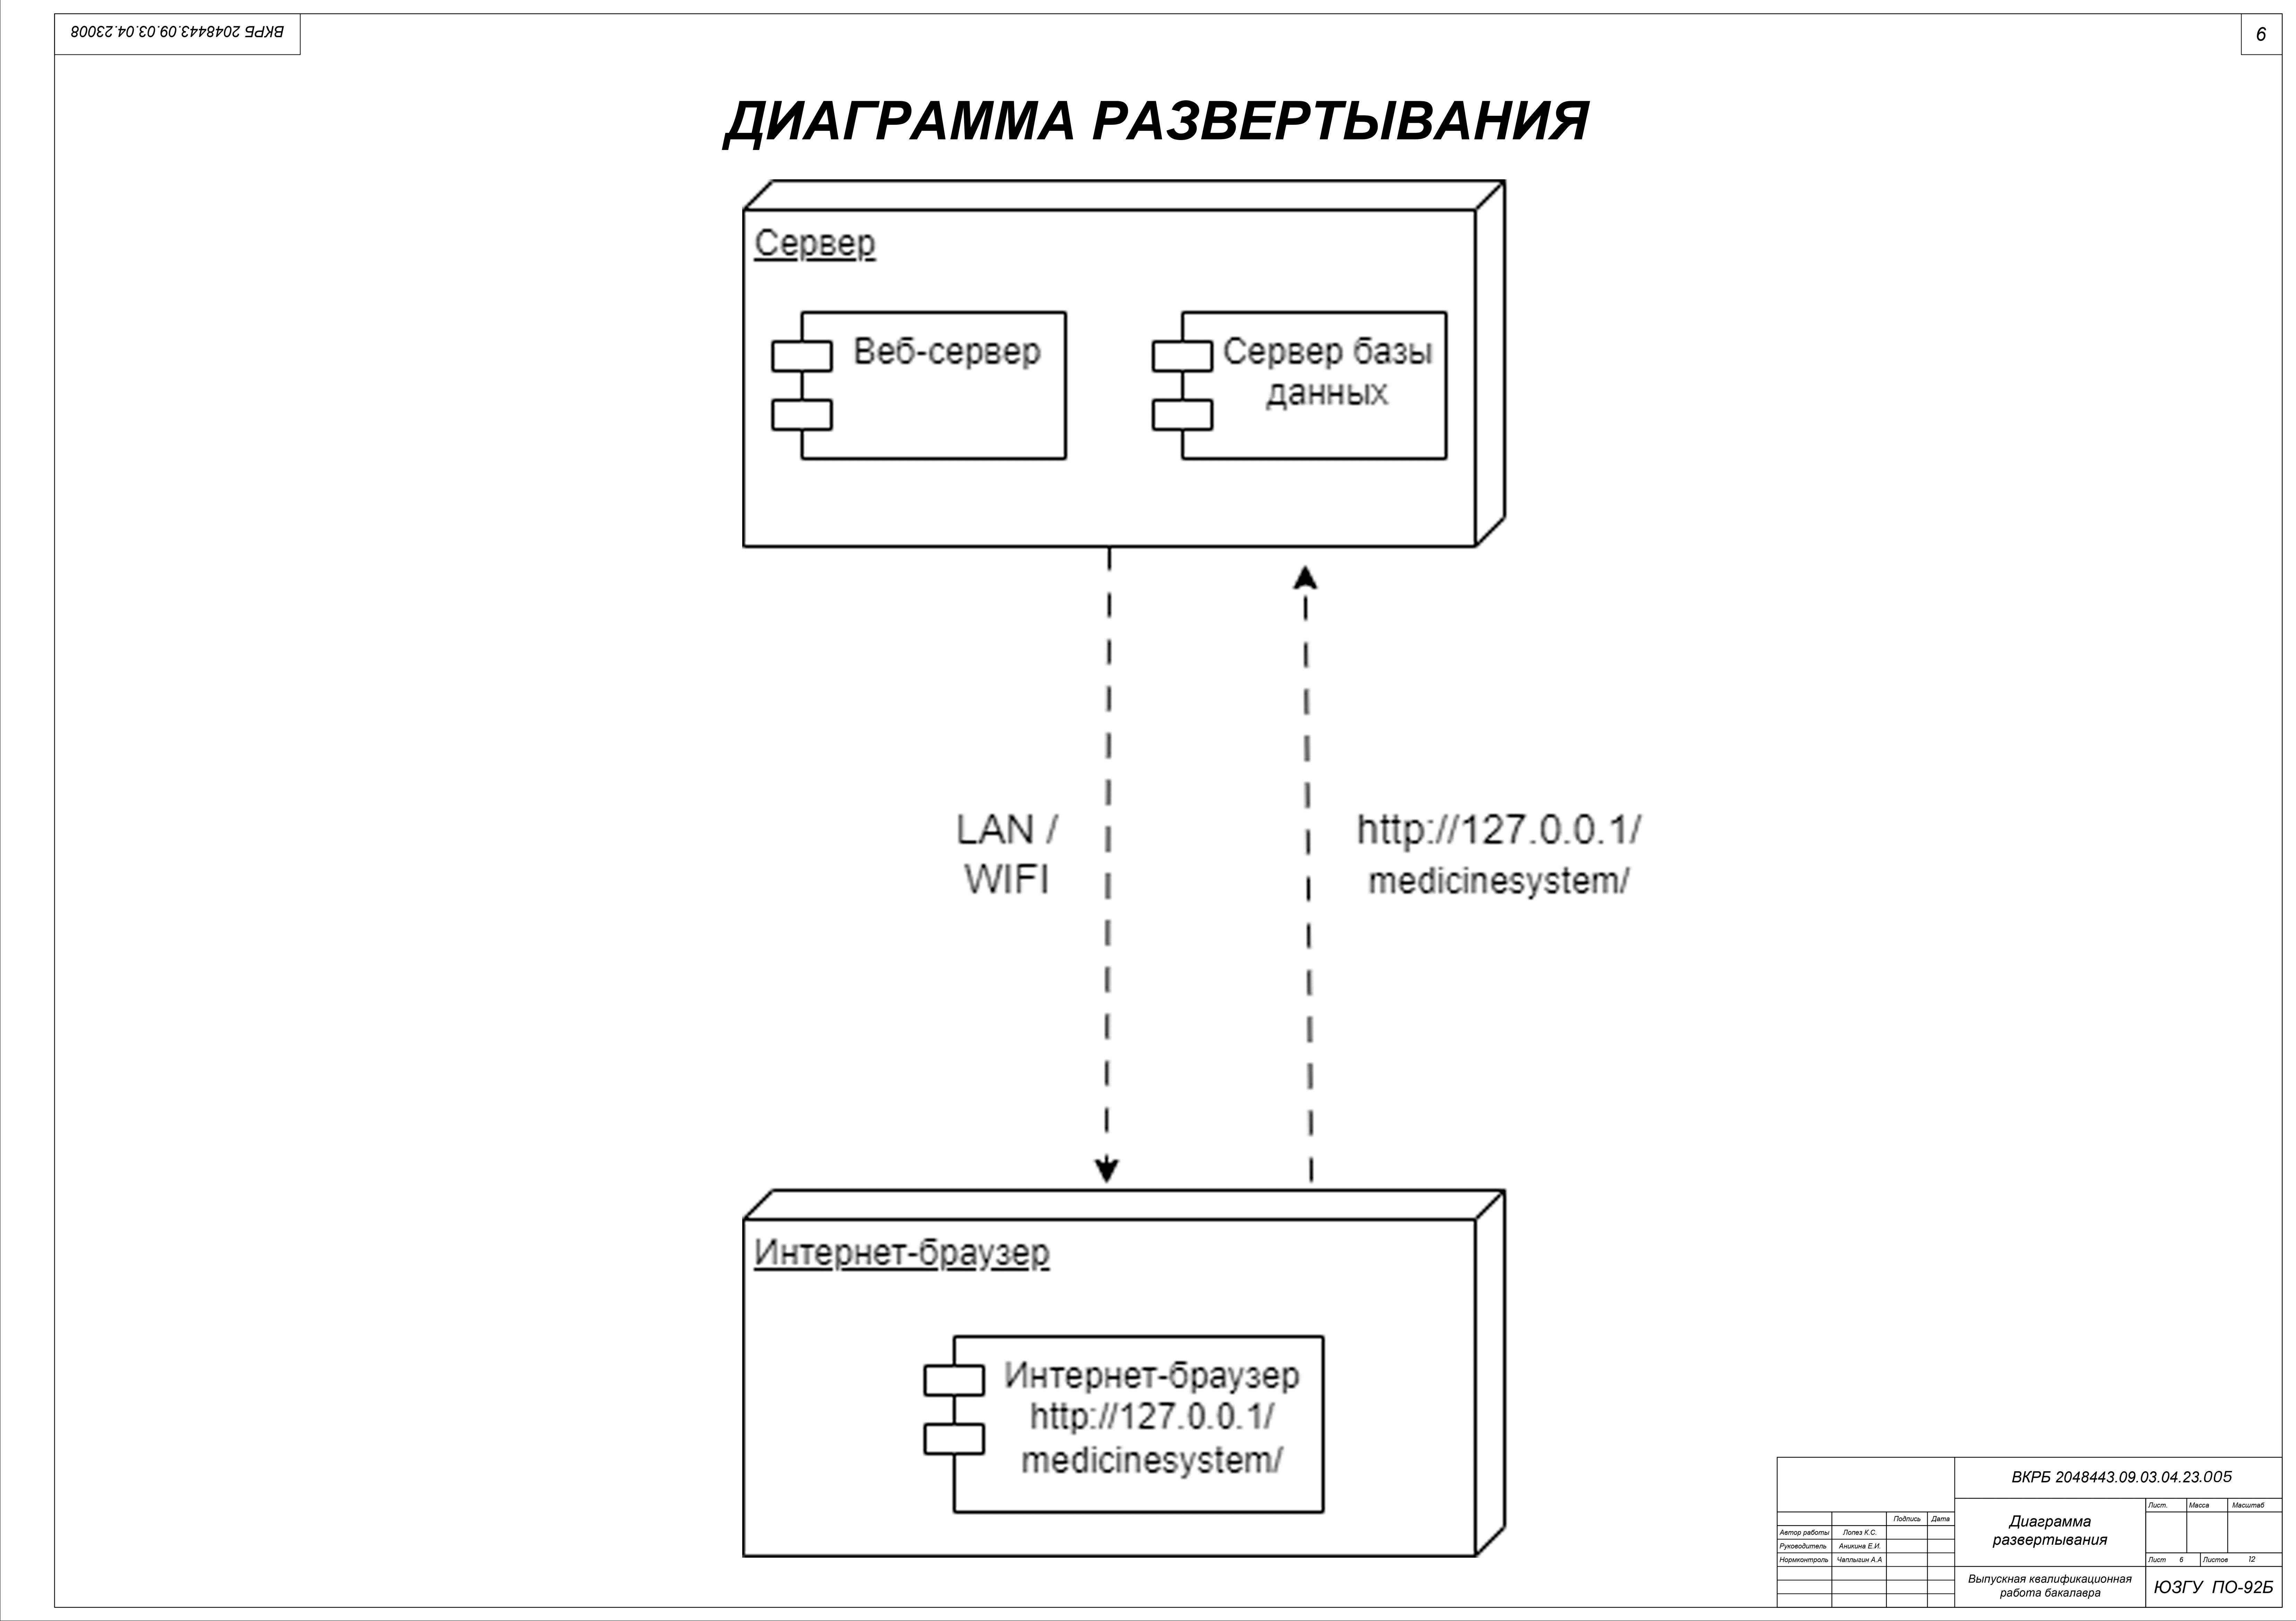
\includegraphics[width=1.3\linewidth]{плакат6.png}
	\end{adjustbox}
	\label{pl6:image}      
\end{figure}

\begin{figure}
	\begin{adjustbox}{addcode={\begin{minipage}{\width}}{\caption{%
						Диаграмма классов
			}\end{minipage}},rotate=90,center}
		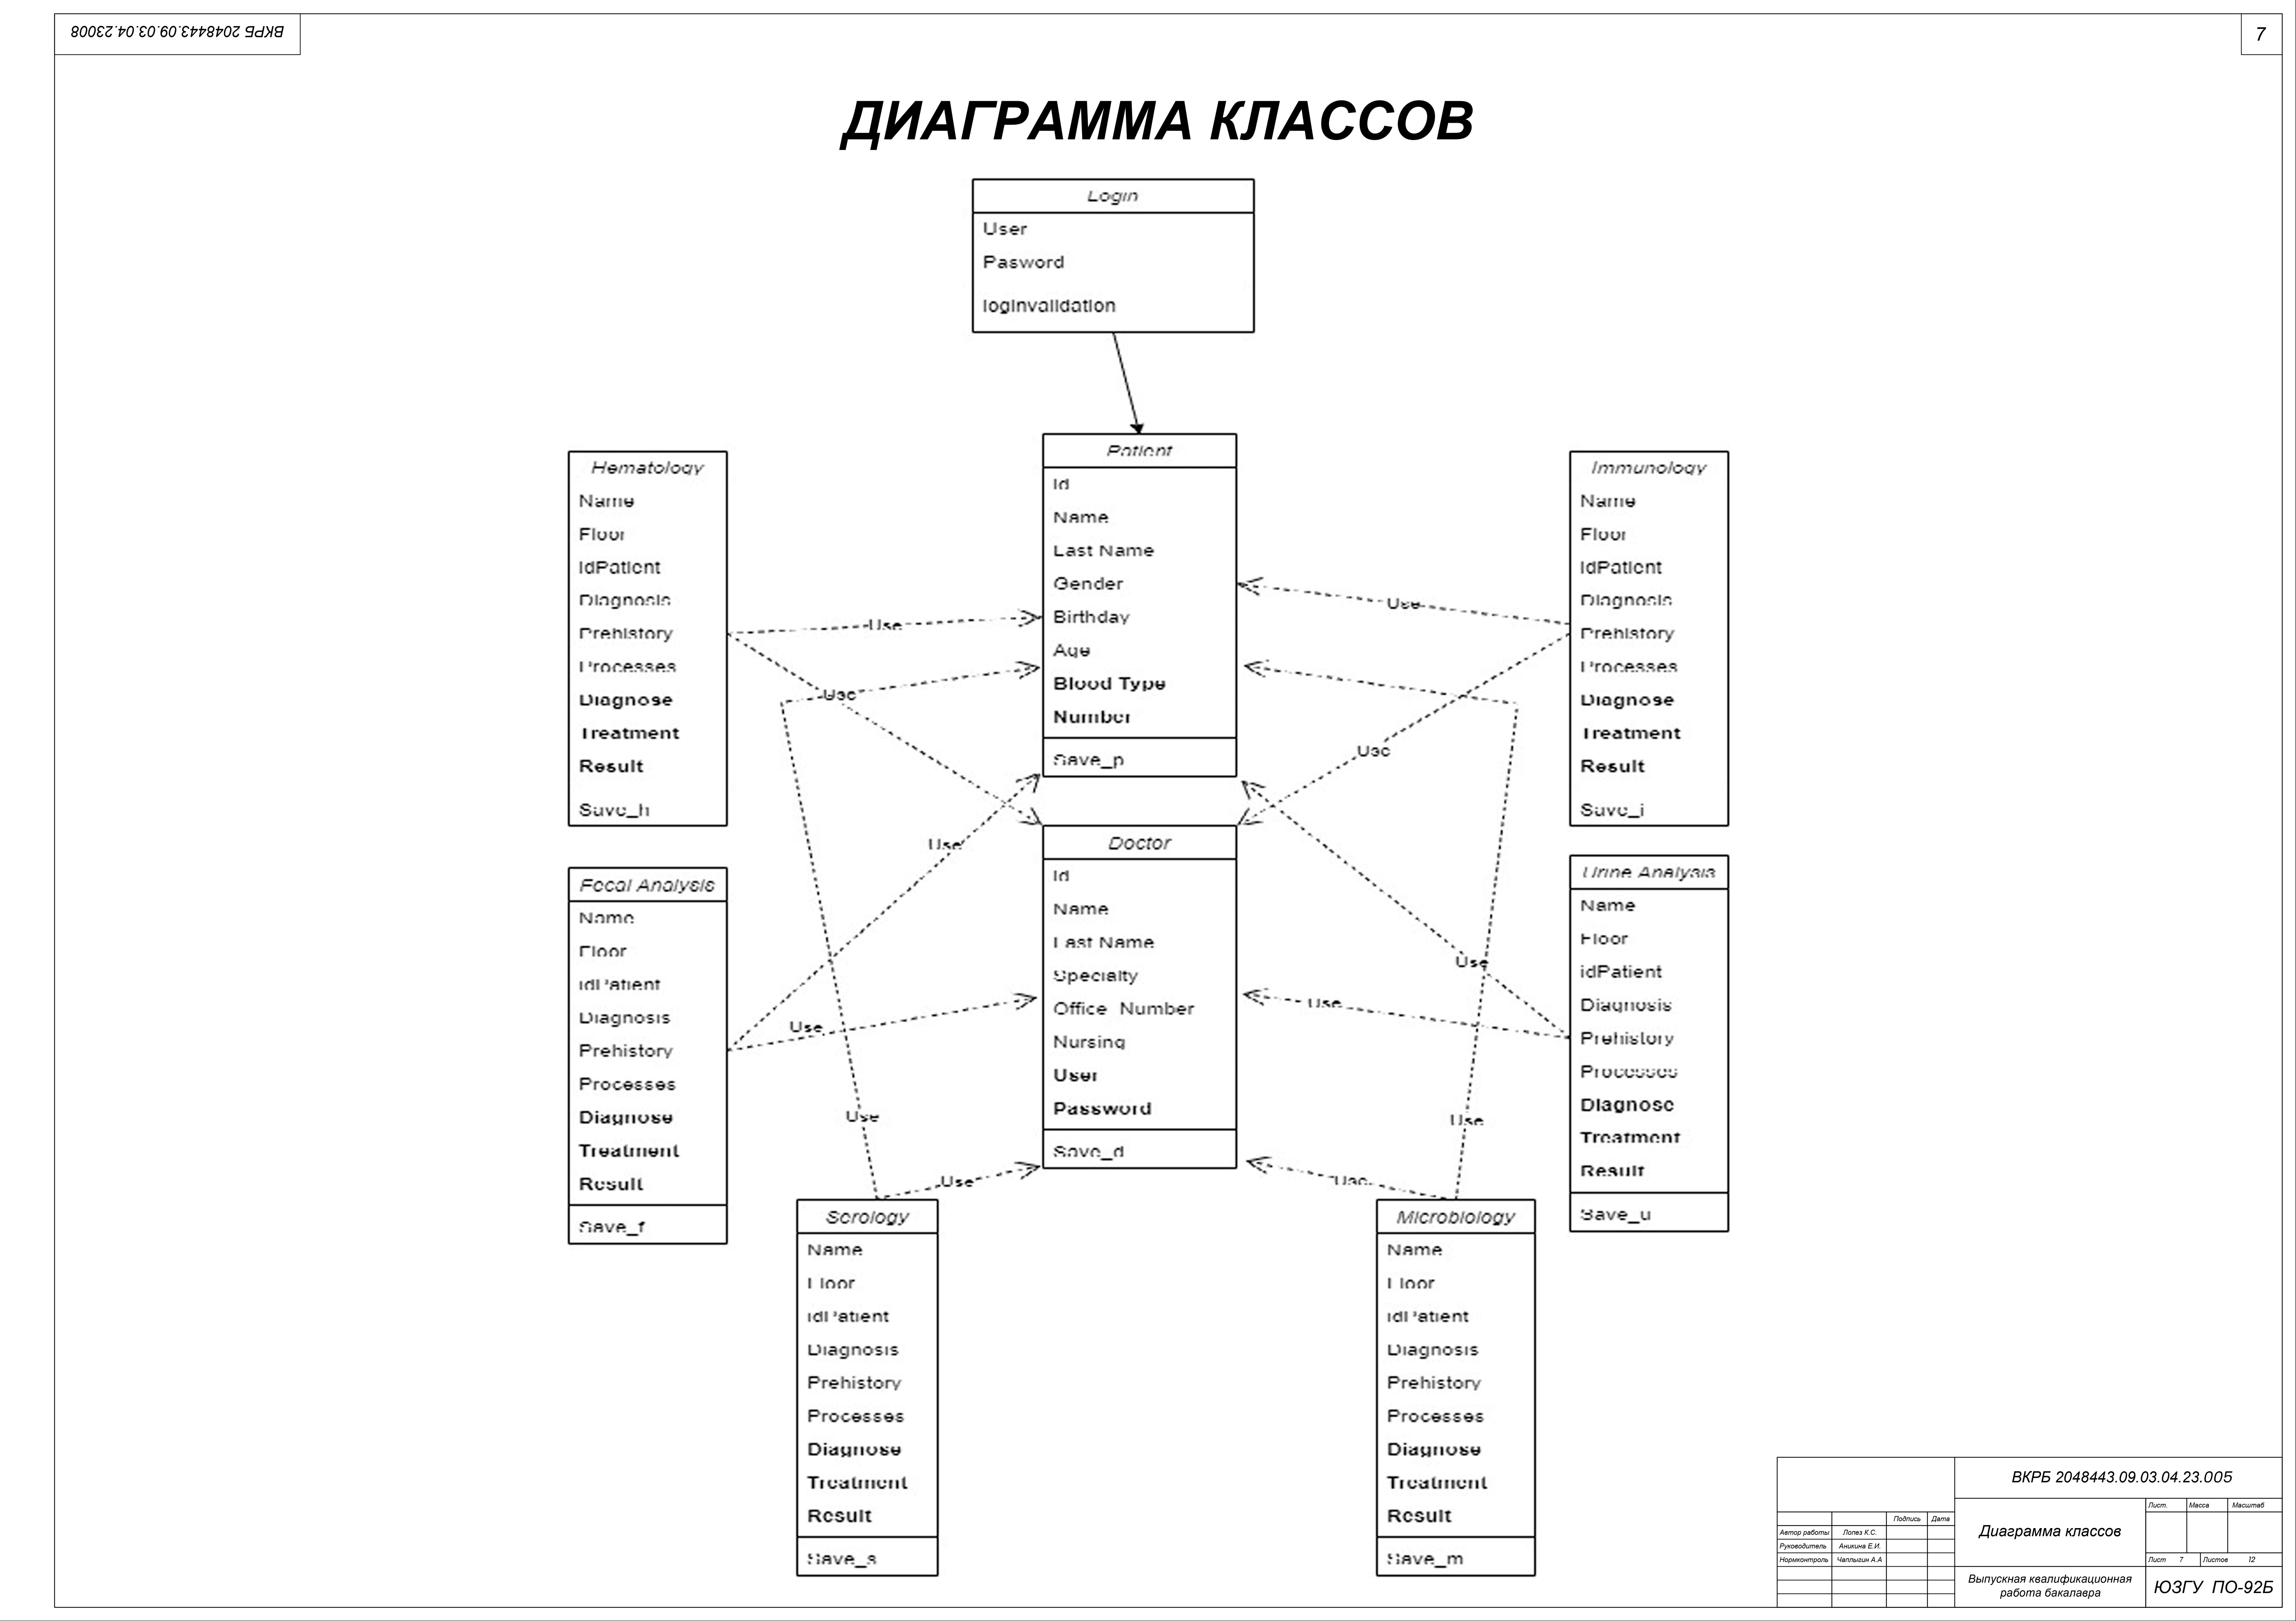
\includegraphics[width=1.3\linewidth]{плакат7.png}
	\end{adjustbox}
	\label{pl7:image}      
\end{figure}

\begin{figure}
	\begin{adjustbox}{addcode={\begin{minipage}{\width}}{\caption{%
						Дизайн интерфейса. Веб-страница авторизации
			}\end{minipage}},rotate=90,center}
		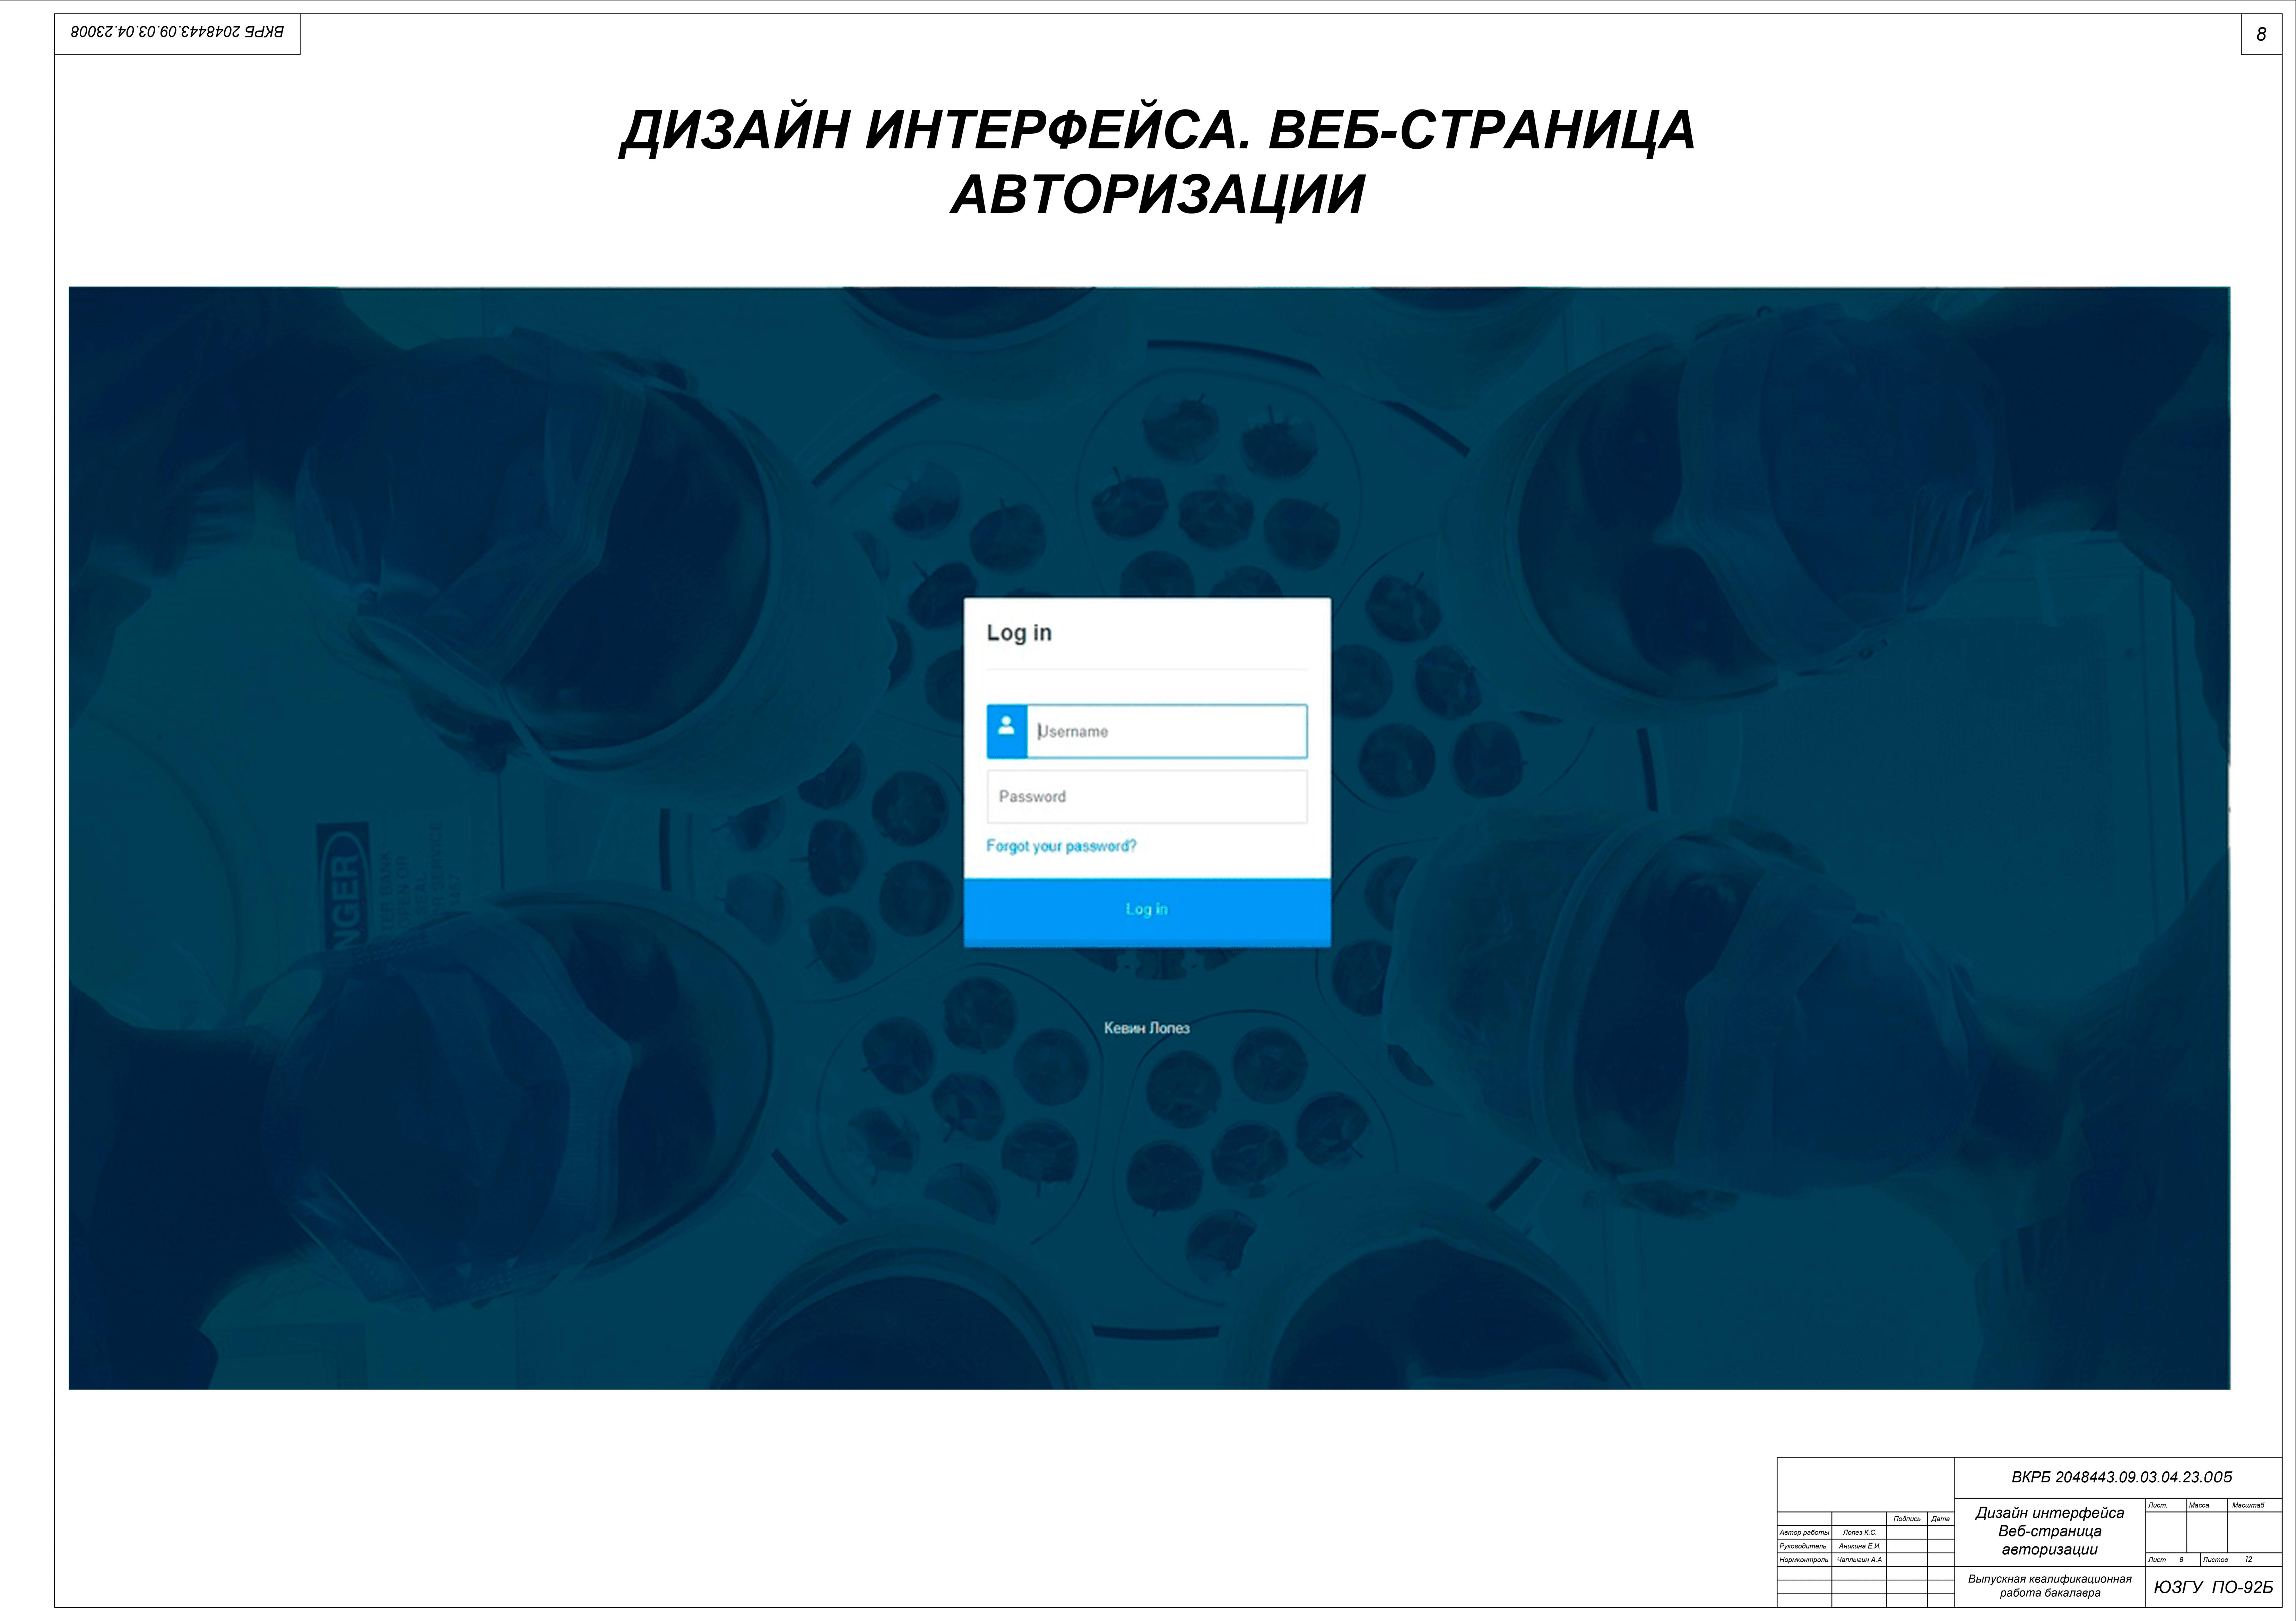
\includegraphics[width=1.3\linewidth]{плакат8.png}
	\end{adjustbox}
	\label{pl8:image}      
\end{figure}

\begin{figure}
	\begin{adjustbox}{addcode={\begin{minipage}{\width}}{\caption{%
						Дизайн интерфейса. Веб-страница регистрации пациента
			}\end{minipage}},rotate=90,center}
		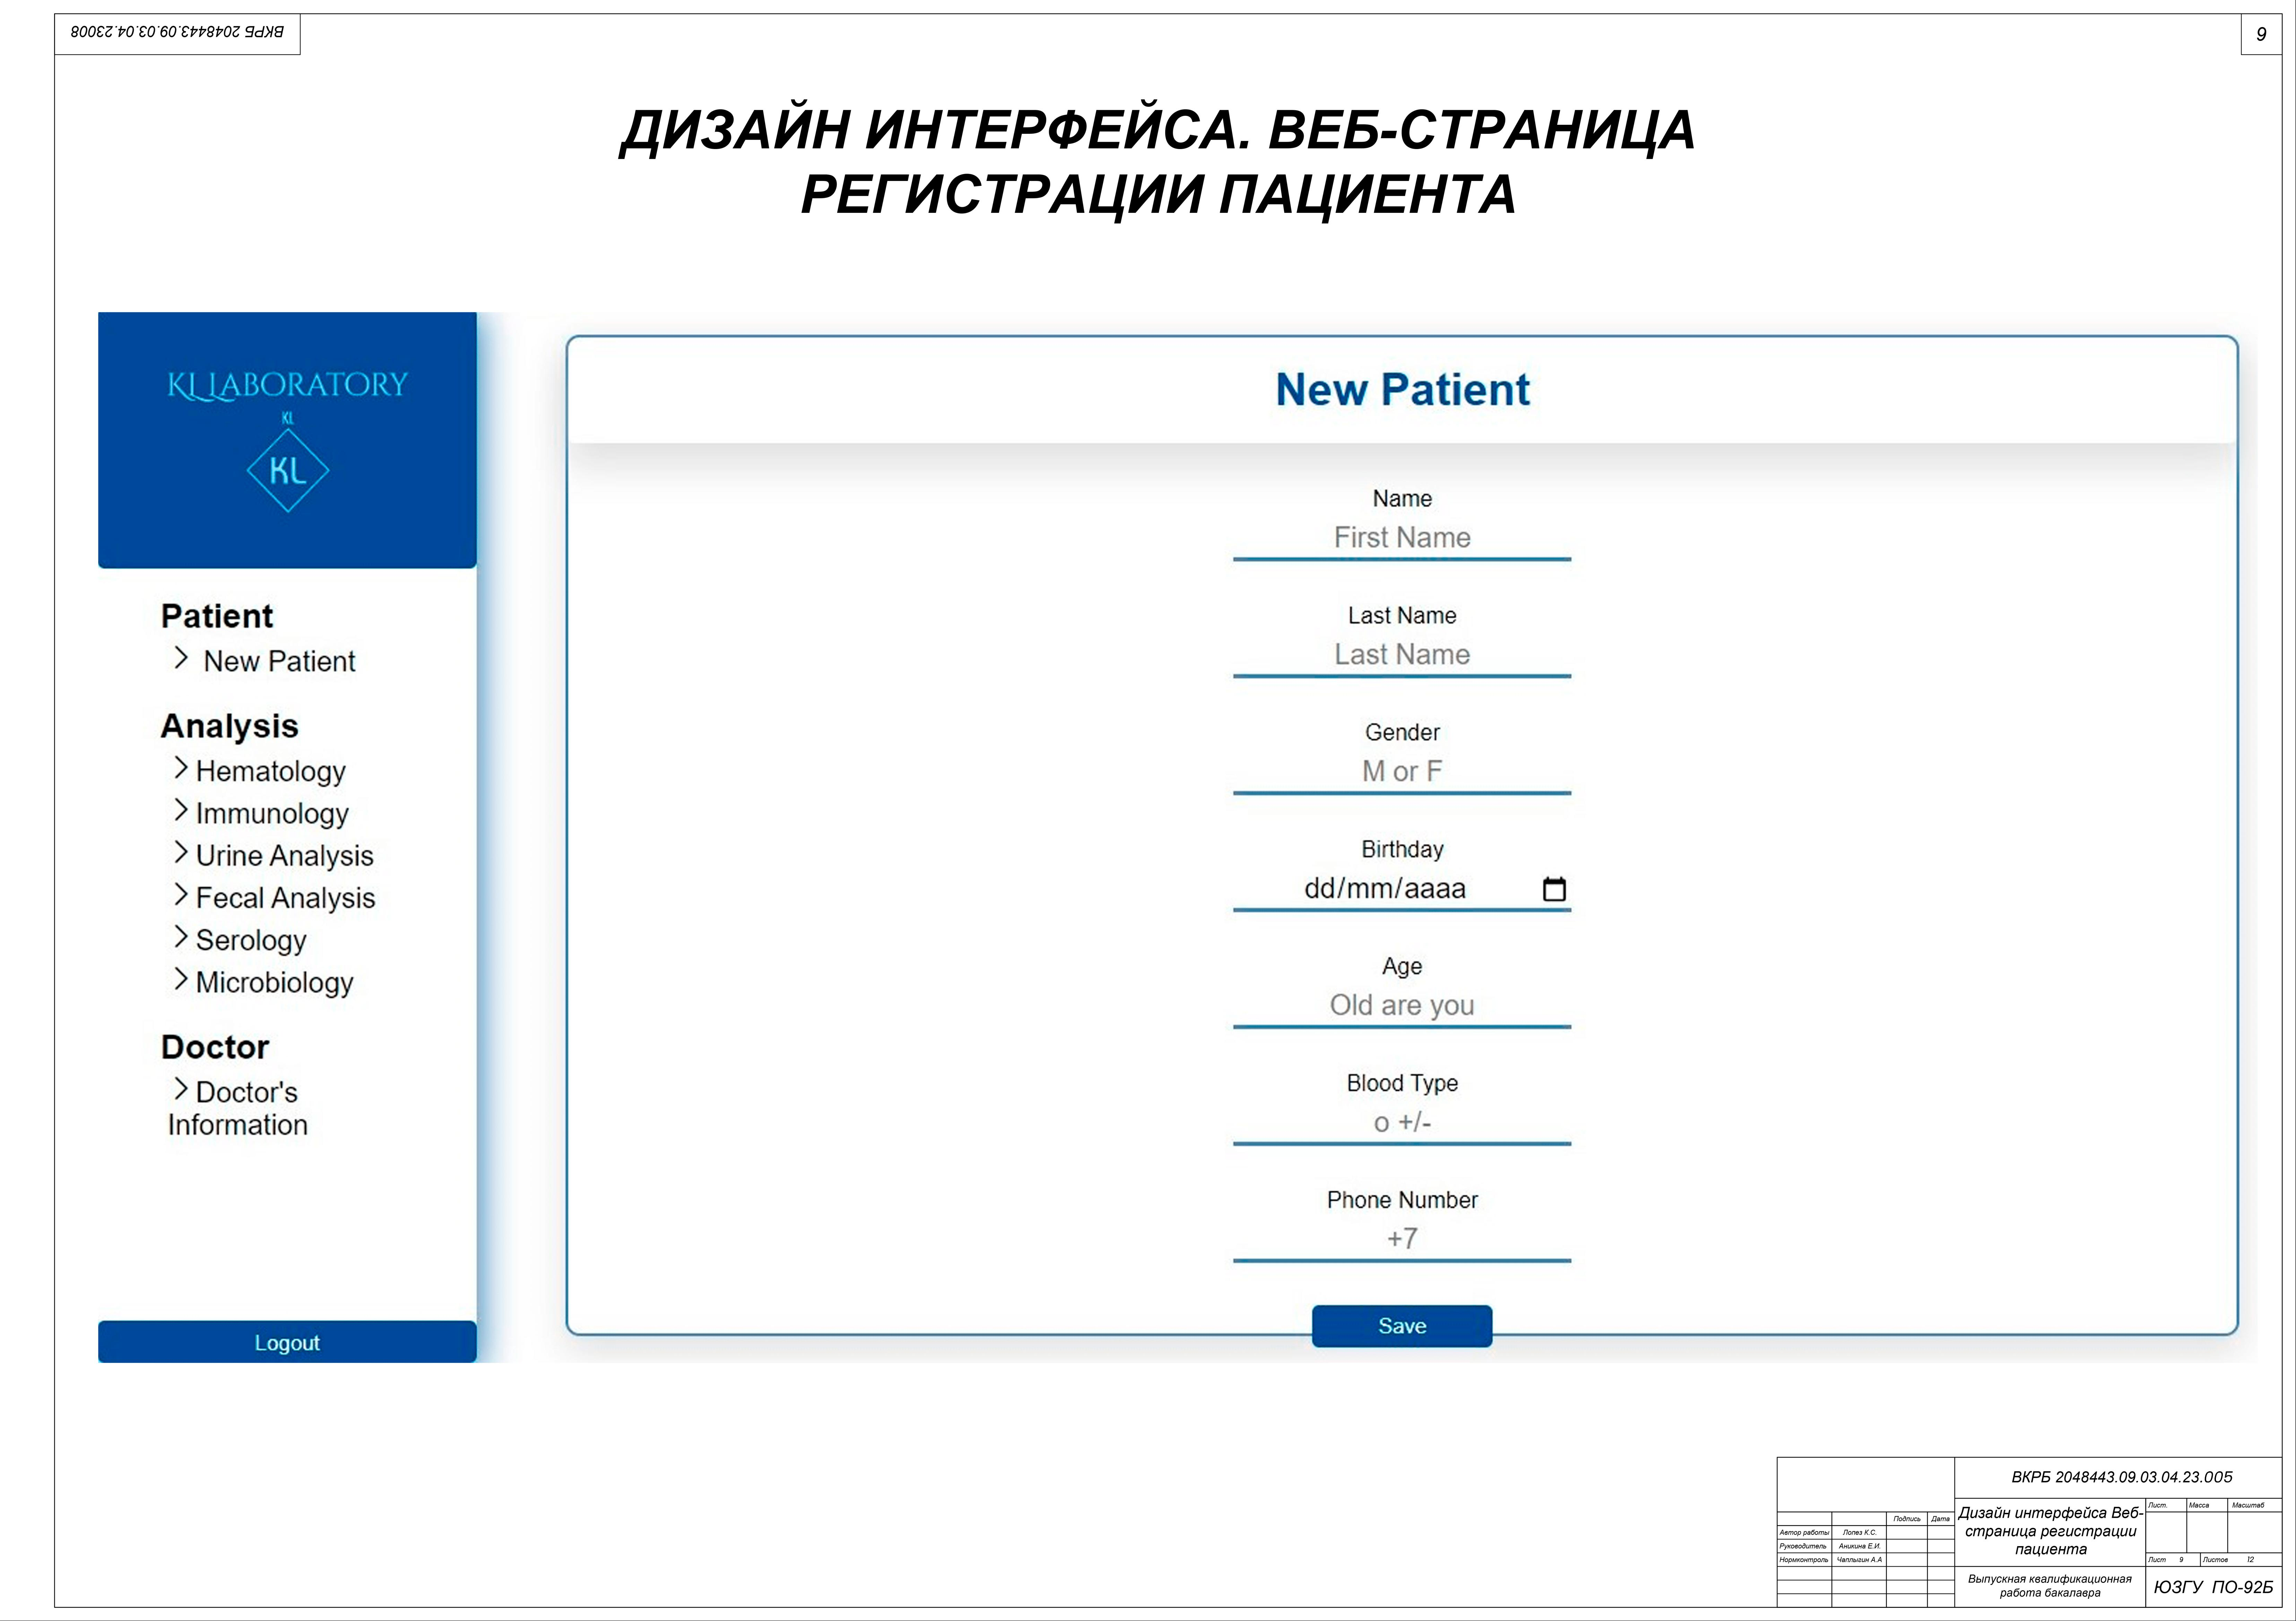
\includegraphics[width=1.3\linewidth]{плакат9.png}
	\end{adjustbox}
	\label{pl9:image}      
\end{figure}

\begin{figure}
	\begin{adjustbox}{addcode={\begin{minipage}{\width}}{\caption{%
						Дизайн интерфейса. Веб-страница регистрации врача
			}\end{minipage}},rotate=90,center}
		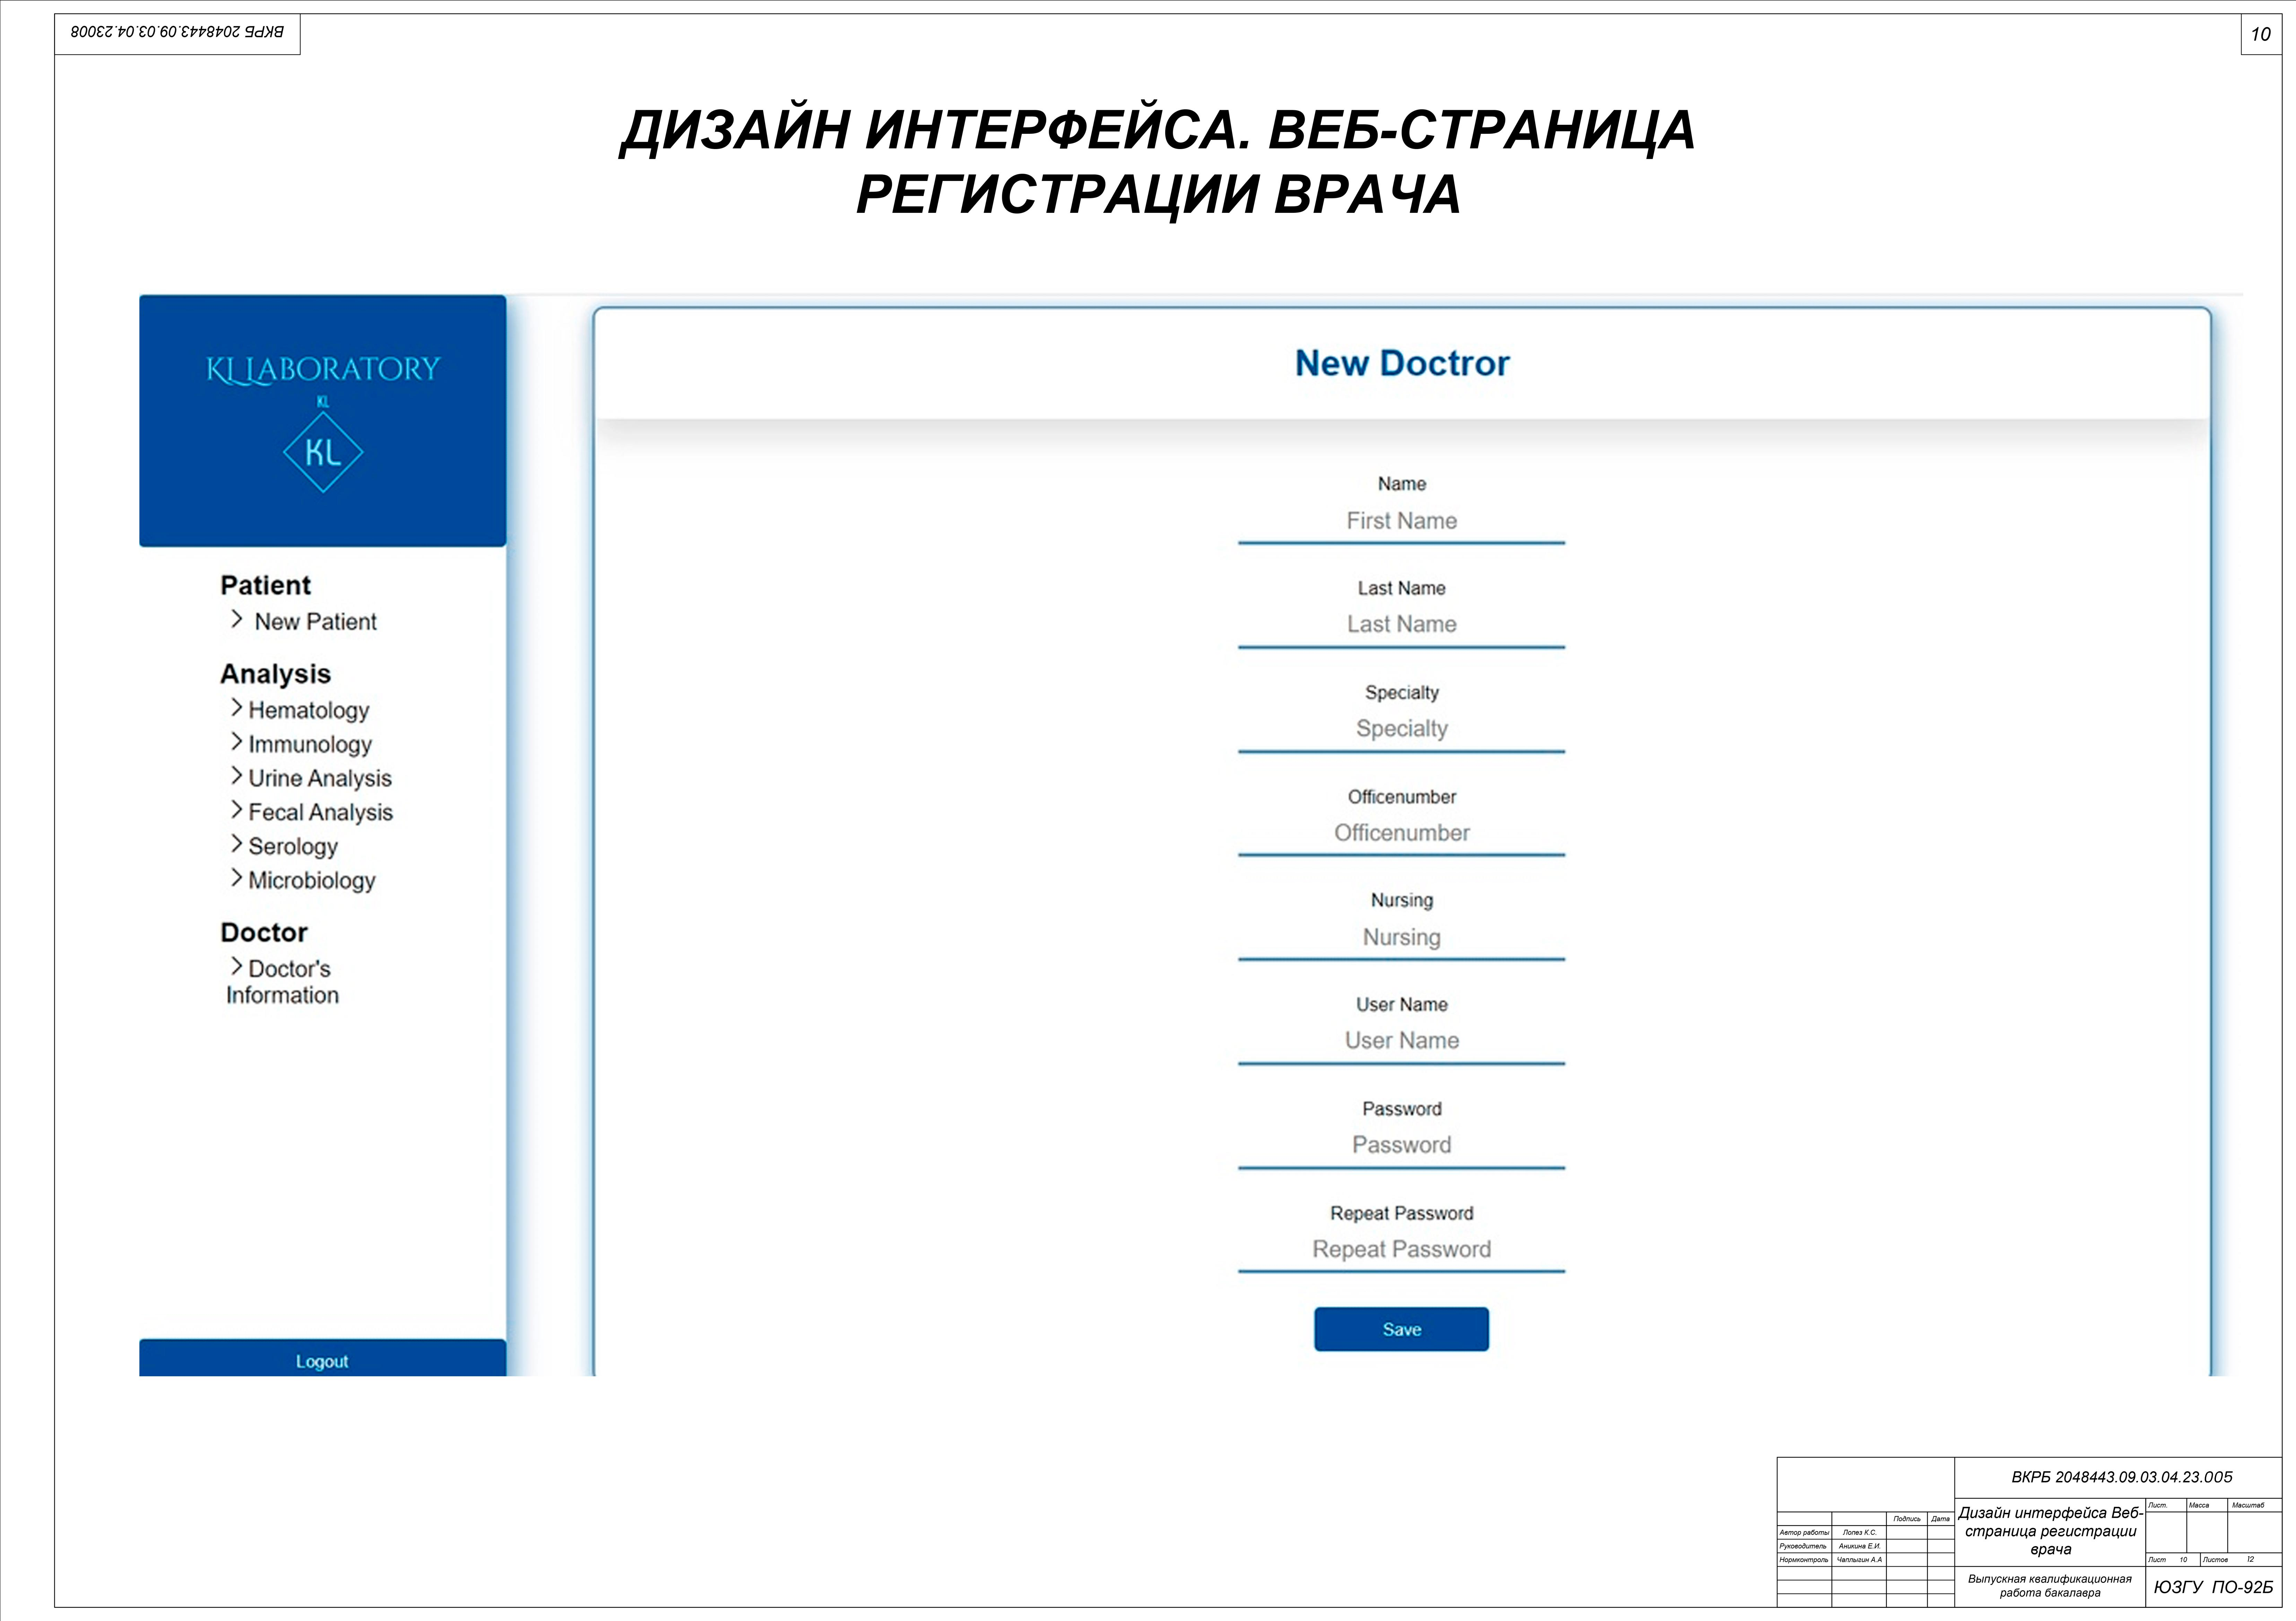
\includegraphics[width=1.3\linewidth]{плакат10.png}
	\end{adjustbox}
	\label{pl10:image}      
\end{figure}

\begin{figure}
	\begin{adjustbox}{addcode={\begin{minipage}{\width}}{\caption{%
						Дизайн интерфейса. Веб-страница для ввода результатов анализа крови
			}\end{minipage}},rotate=90,center}
		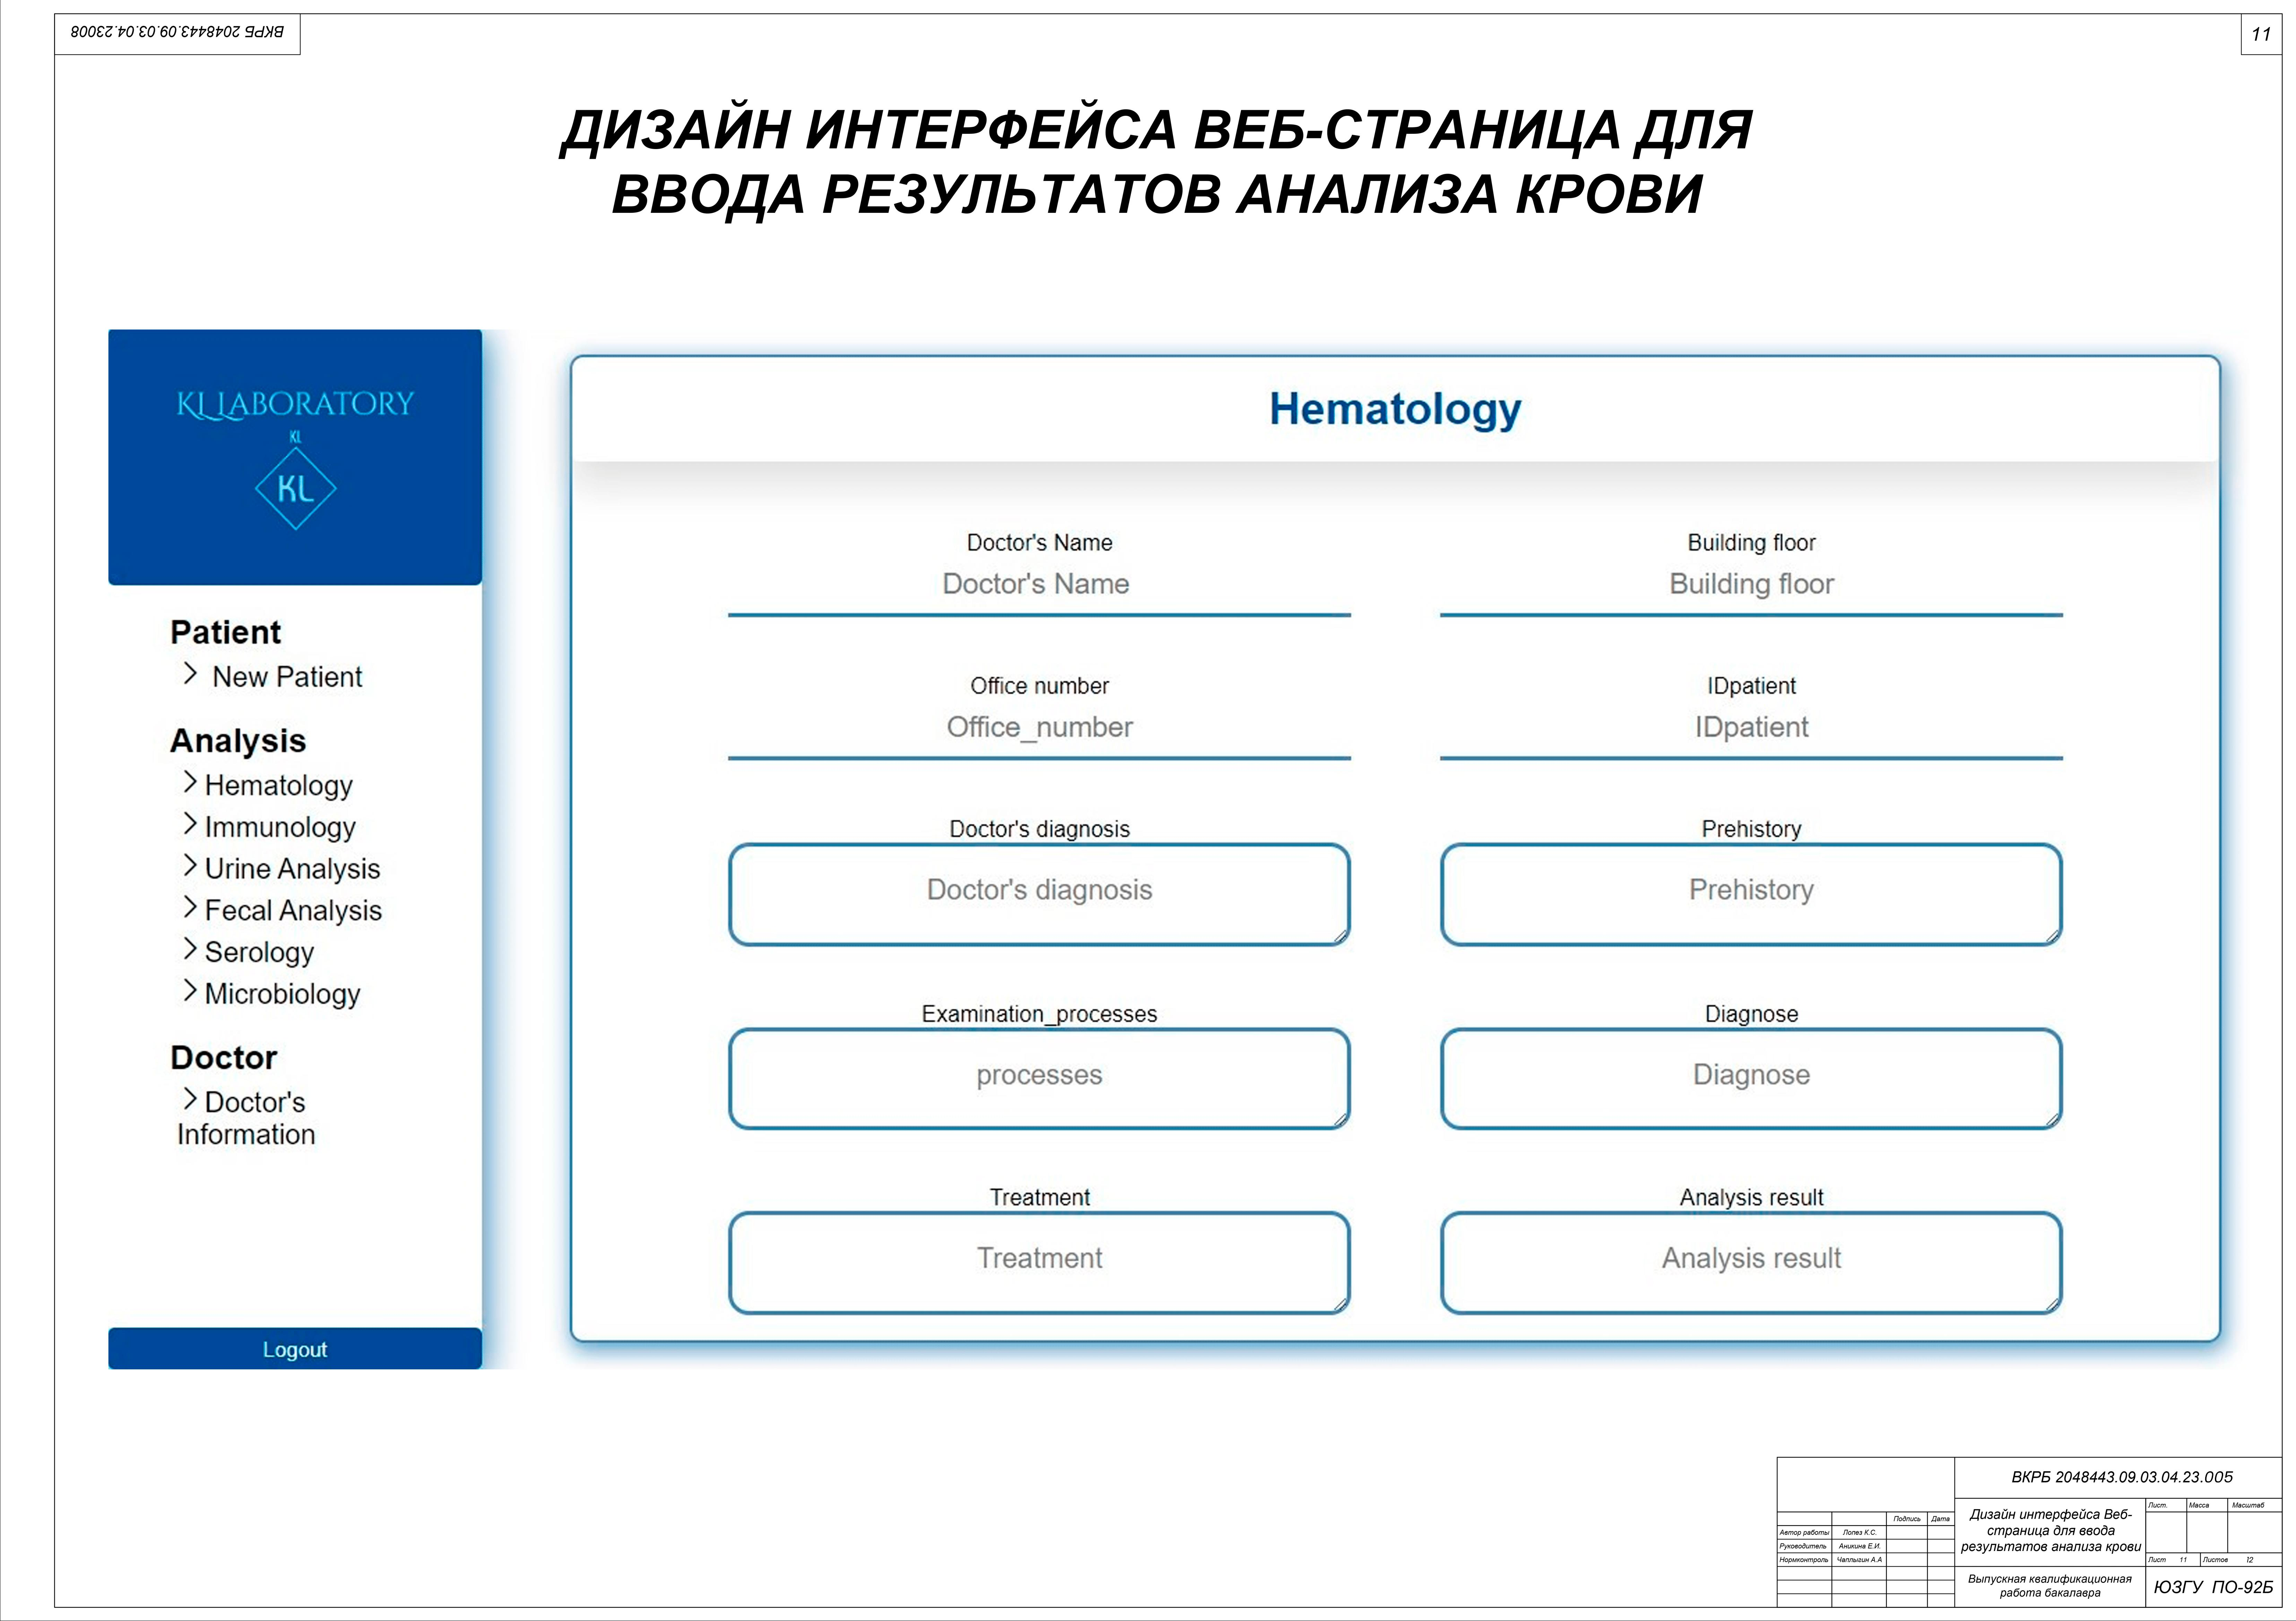
\includegraphics[width=1.3\linewidth]{плакат11.png}
	\end{adjustbox}
	\label{pl11:image}      
\end{figure}

\begin{figure}
	\begin{adjustbox}{addcode={\begin{minipage}{\width}}{\caption{%
						Заключение
			}\end{minipage}},rotate=90,center}
		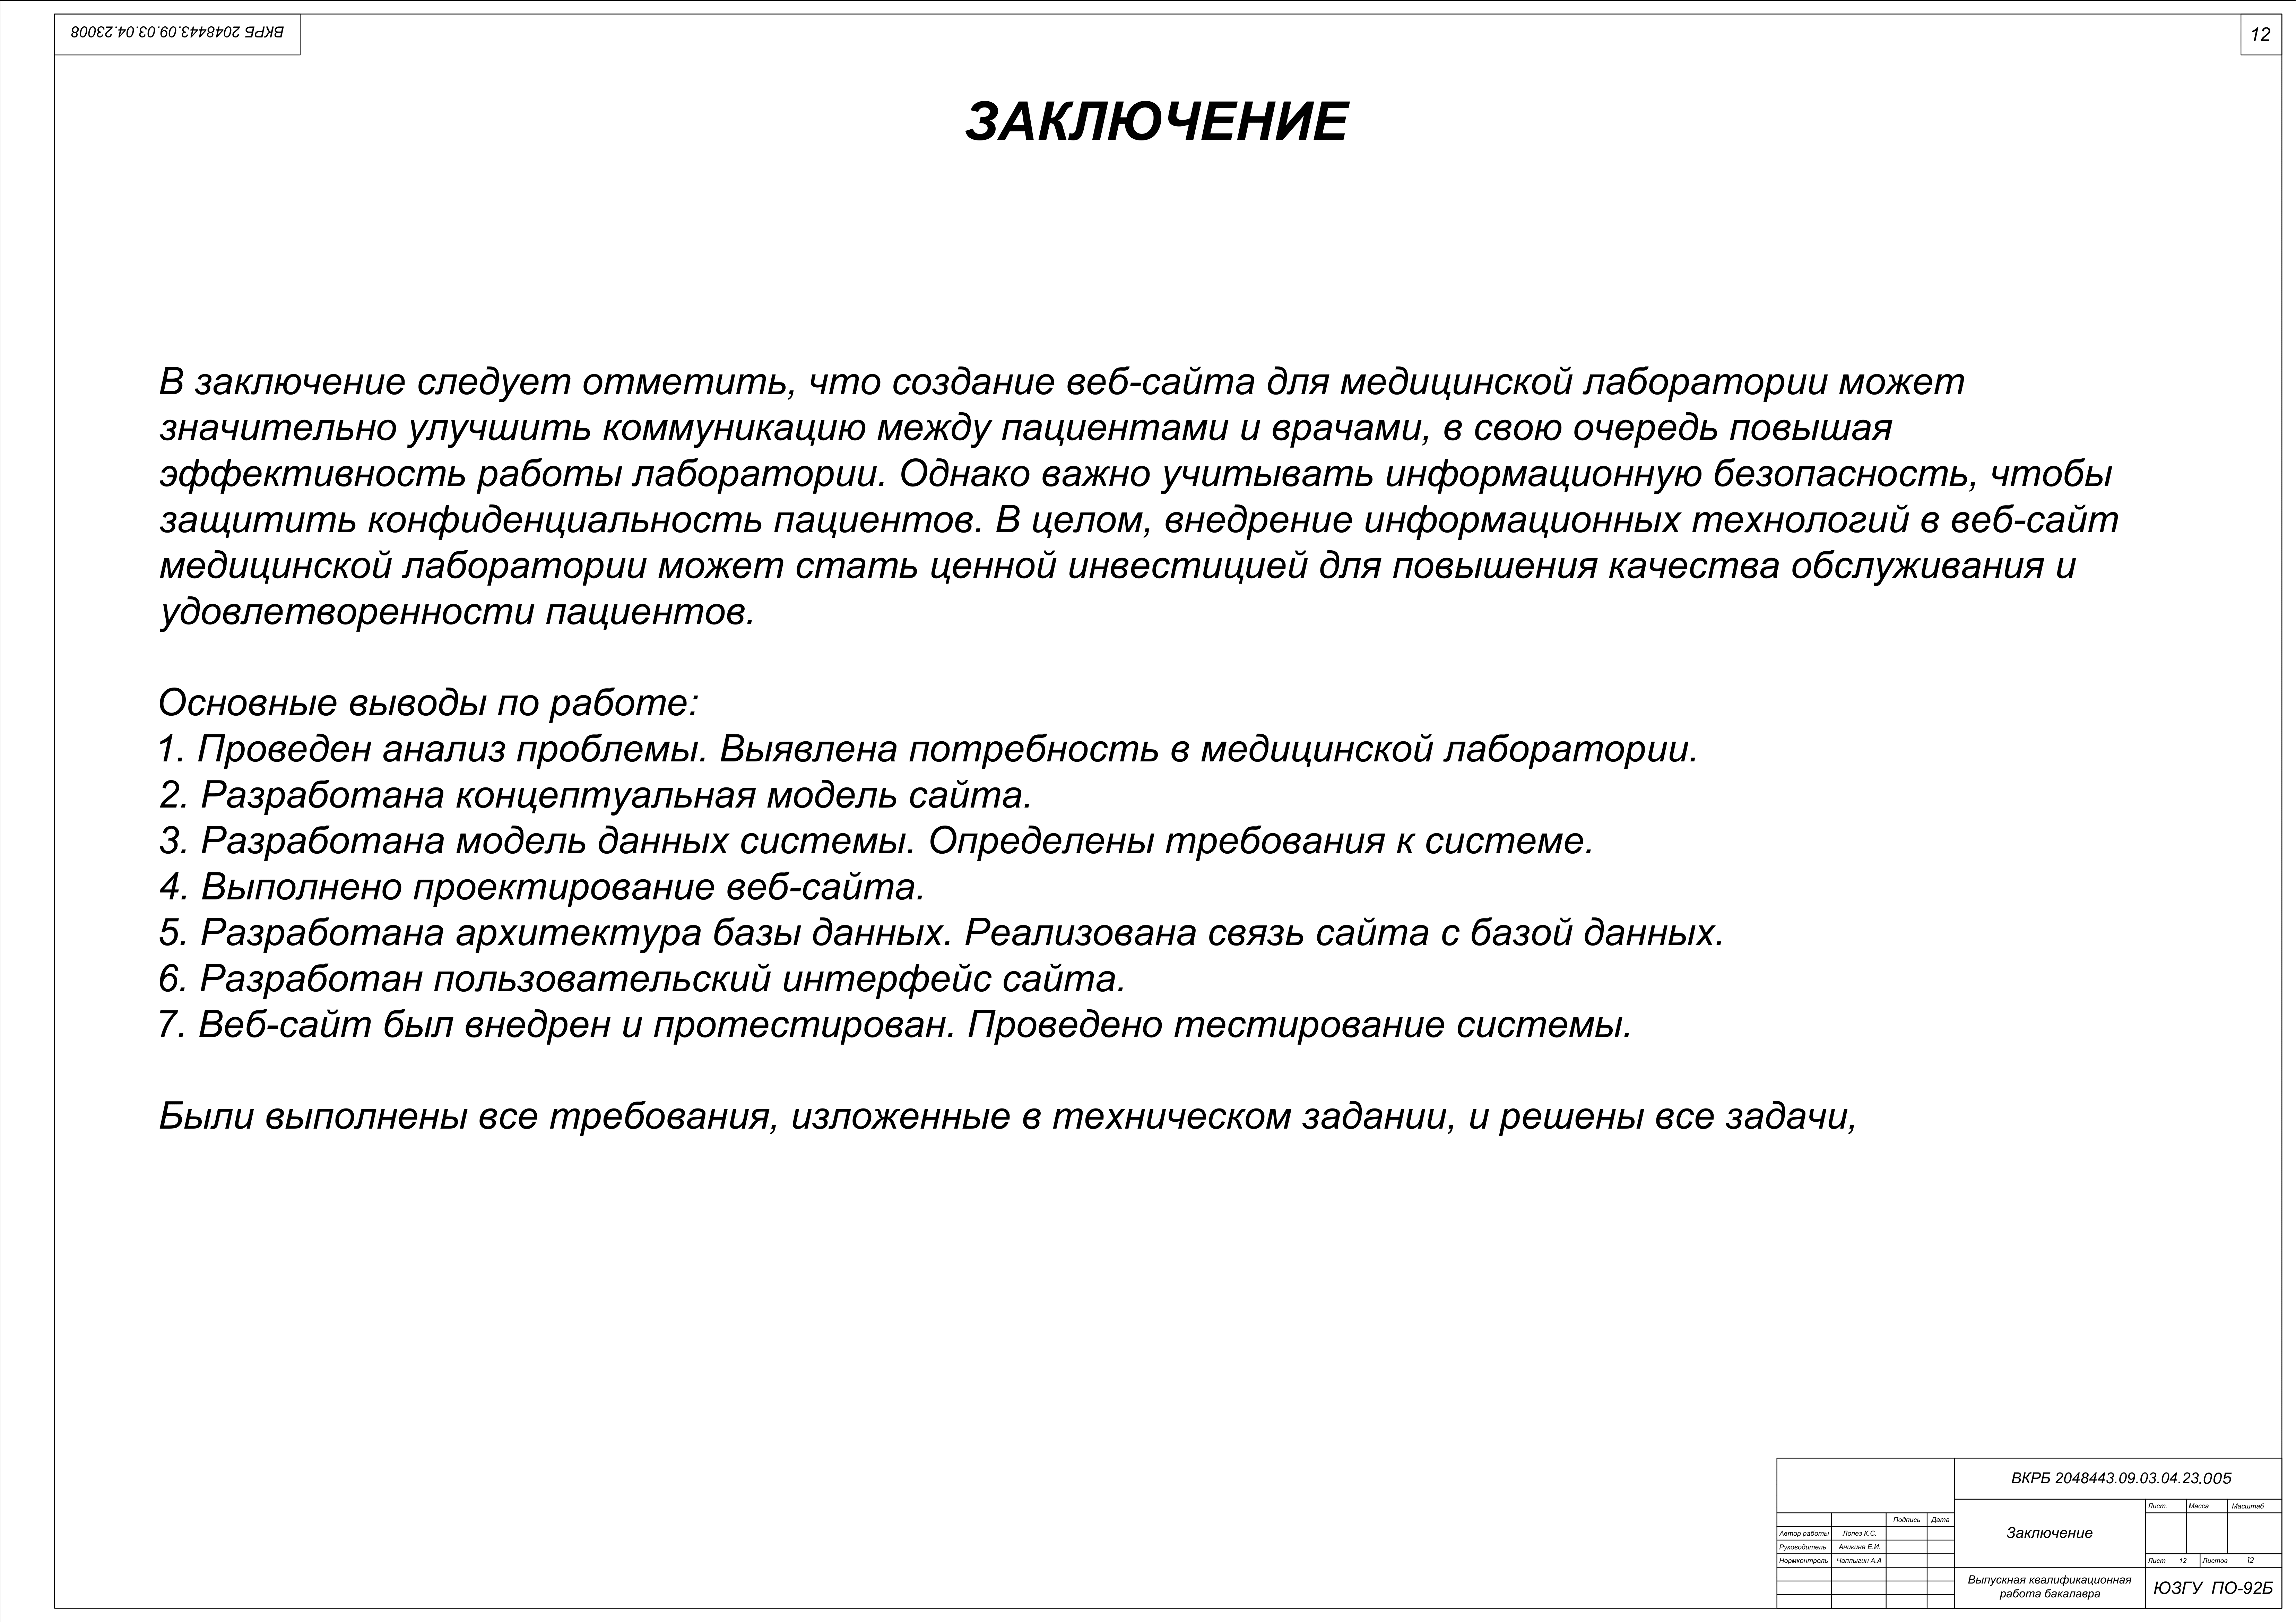
\includegraphics[width=1.3\linewidth]{плакат12.png}
	\end{adjustbox}
	\label{pl12:image}      
\end{figure}
	\newsection
\section*{ПРИЛОЖЕНИЕ Б \\ Фрагменты исходного кода программы}\label{ПРИЛОЖЕНИЕ}
\addcontentsline{toc}{section}{ПРИЛОЖЕНИЕ Б Фрагменты исходного кода программы}

Кодlogin.tex
\lstinputlisting[language=Tex, frame=none]{Кодlogin.tex}

КодDoctors.tex
\lstinputlisting[language=Tex, frame=none]{КодDoctors.tex}

\newpage
КодPatient.tex
\lstinputlisting[language=Tex, frame=none]{КодPatient.tex}

\newpage
КодFormulario.tex
\lstinputlisting[language=Tex, frame=none]{КодFormulario.tex}

\newpage
\addcontentsline{toc}{section}{На отдельных листах (CD-RW в прикрепленном конверте)}

\begin{center}
\textbf{Место для диска}
\end{center}

\end{document}
